% Options for packages loaded elsewhere
\PassOptionsToPackage{unicode}{hyperref}
\PassOptionsToPackage{hyphens}{url}
%
\documentclass[
]{book}
\usepackage{lmodern}
\usepackage{amssymb,amsmath}
\usepackage{ifxetex,ifluatex}
\ifnum 0\ifxetex 1\fi\ifluatex 1\fi=0 % if pdftex
  \usepackage[T1]{fontenc}
  \usepackage[utf8]{inputenc}
  \usepackage{textcomp} % provide euro and other symbols
\else % if luatex or xetex
  \usepackage{unicode-math}
  \defaultfontfeatures{Scale=MatchLowercase}
  \defaultfontfeatures[\rmfamily]{Ligatures=TeX,Scale=1}
\fi
% Use upquote if available, for straight quotes in verbatim environments
\IfFileExists{upquote.sty}{\usepackage{upquote}}{}
\IfFileExists{microtype.sty}{% use microtype if available
  \usepackage[]{microtype}
  \UseMicrotypeSet[protrusion]{basicmath} % disable protrusion for tt fonts
}{}
\makeatletter
\@ifundefined{KOMAClassName}{% if non-KOMA class
  \IfFileExists{parskip.sty}{%
    \usepackage{parskip}
  }{% else
    \setlength{\parindent}{0pt}
    \setlength{\parskip}{6pt plus 2pt minus 1pt}}
}{% if KOMA class
  \KOMAoptions{parskip=half}}
\makeatother
\usepackage{xcolor}
\IfFileExists{xurl.sty}{\usepackage{xurl}}{} % add URL line breaks if available
\IfFileExists{bookmark.sty}{\usepackage{bookmark}}{\usepackage{hyperref}}
\hypersetup{
  pdftitle={EasyPeasy},
  pdfauthor={Hackauthor²},
  hidelinks,
  pdfcreator={LaTeX via pandoc}}
\urlstyle{same} % disable monospaced font for URLs
\usepackage{longtable,booktabs}
% Correct order of tables after \paragraph or \subparagraph
\usepackage{etoolbox}
\makeatletter
\patchcmd\longtable{\par}{\if@noskipsec\mbox{}\fi\par}{}{}
\makeatother
% Allow footnotes in longtable head/foot
\IfFileExists{footnotehyper.sty}{\usepackage{footnotehyper}}{\usepackage{footnote}}
\makesavenoteenv{longtable}
\usepackage{graphicx}
\makeatletter
\def\maxwidth{\ifdim\Gin@nat@width>\linewidth\linewidth\else\Gin@nat@width\fi}
\def\maxheight{\ifdim\Gin@nat@height>\textheight\textheight\else\Gin@nat@height\fi}
\makeatother
% Scale images if necessary, so that they will not overflow the page
% margins by default, and it is still possible to overwrite the defaults
% using explicit options in \includegraphics[width, height, ...]{}
\setkeys{Gin}{width=\maxwidth,height=\maxheight,keepaspectratio}
% Set default figure placement to htbp
\makeatletter
\def\fps@figure{htbp}
\makeatother
\setlength{\emergencystretch}{3em} % prevent overfull lines
\providecommand{\tightlist}{%
  \setlength{\itemsep}{0pt}\setlength{\parskip}{0pt}}
\setcounter{secnumdepth}{5}
\usepackage{booktabs}

\usepackage[T1]{fontenc}
\usepackage[a4paper, margin=2cm]{geometry}

%\usepackage{titling}
%\usepackage[sfdefault,scaled=.90]{FiraSans}
%\usepackage{newtxsf}
%\usepackage{ragged2e}
\ifluatex
  \usepackage{selnolig}  % disable illegal ligatures
\fi
\usepackage[]{natbib}
\bibliographystyle{apalike}

\title{EasyPeasy}
\author{Hackauthor²}
\date{2020-11-11}

\begin{document}
\maketitle

{
\setcounter{tocdepth}{1}
\tableofcontents
}
\hypertarget{preface}{%
\chapter*{Preface}\label{preface}}
\addcontentsline{toc}{chapter}{Preface}

\begin{figure}
\centering
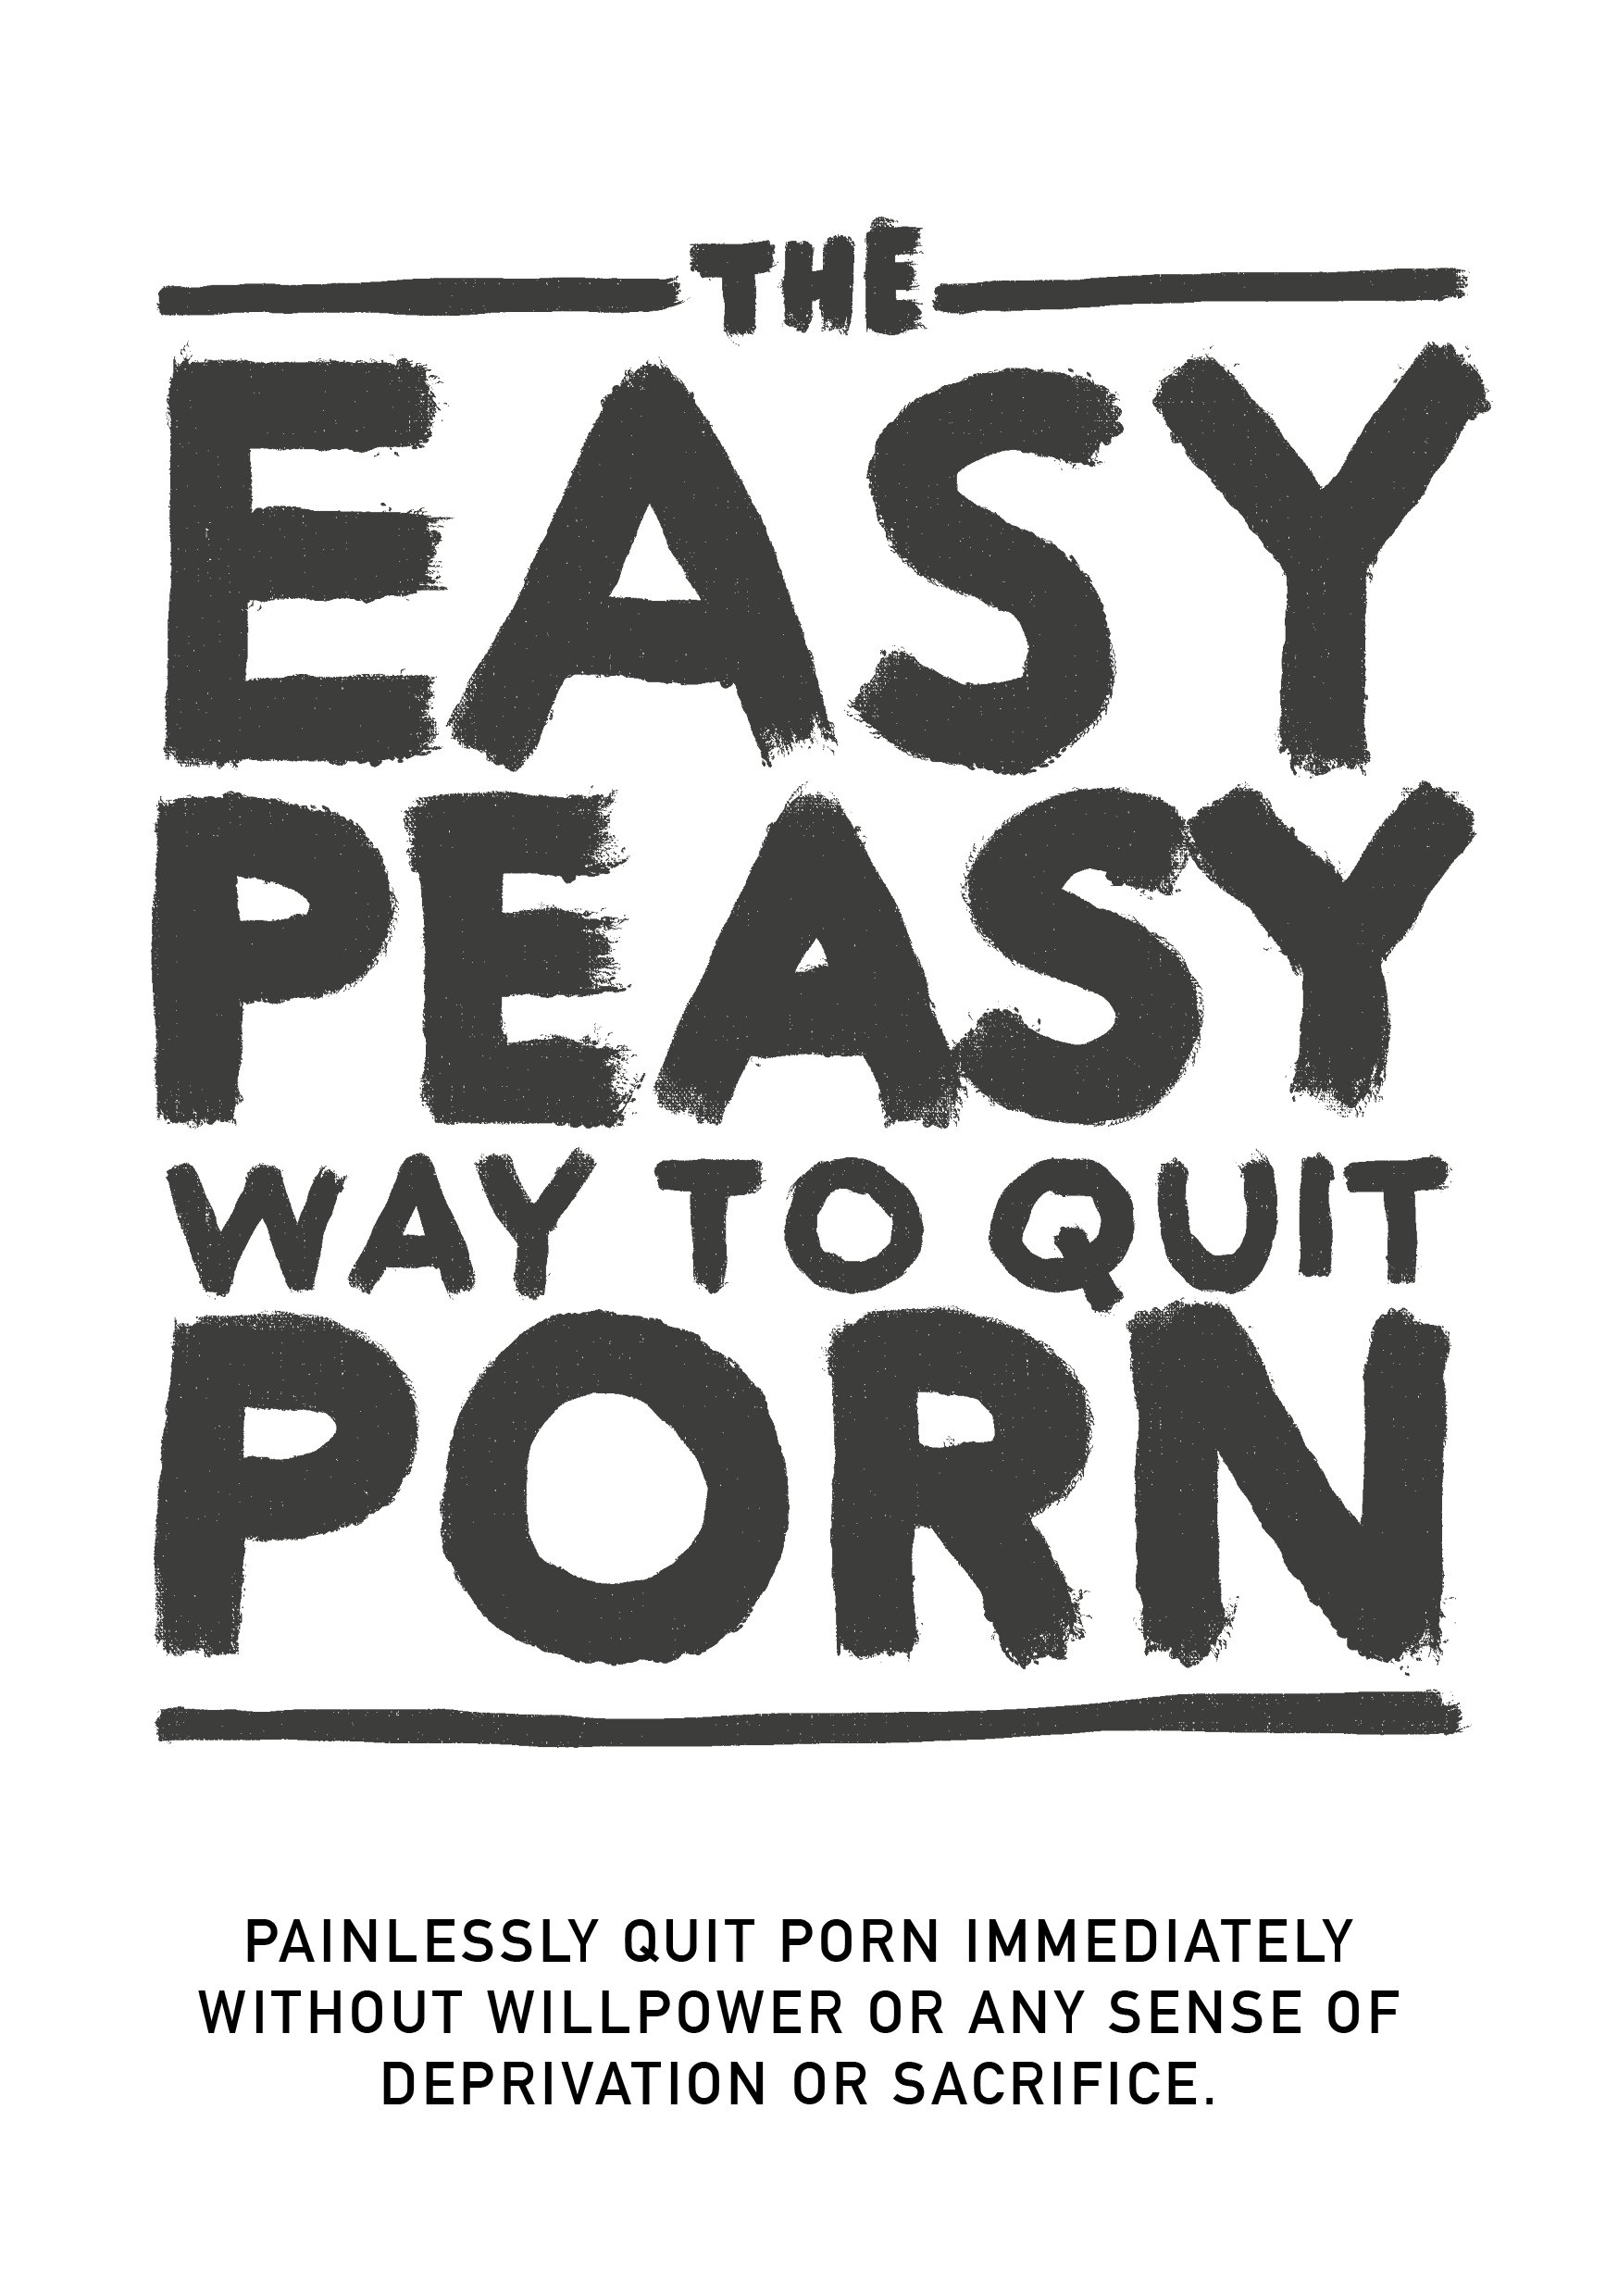
\includegraphics[width=0.45\textwidth,height=0.45\textheight]{images/easypeasy.jpg}
\caption{Cover Image}
\end{figure}

{\textbf{DO NOT JUMP CHAPTERS}}

\textbf{\emph{Painlessly quit porn immediately, without willpower or any sense of deprivation or sacrifice.}}

This is a rewritten version of a \href{https://sites.google.com/site/hackbookeasypeasy}{rewrite} adapting \emph{Allen Carr's EasyWay to Stop Smoking} for pornography. It's also \textbf{completely free} and \href{https://gitlab.com/snuggy/easypeasy}{open source}. I'm not the original author of either of these books, I'm the Hackauthor².

It's very effective, but critical to your success requires that you:

{\textbf{DO NOT JUMP CHAPTERS}}

When opening a combination lock, you have to enter the numbers in the right order. Addiction isn't any different.

Personally, the \href{https://sites.google.com/site/hackbookeasypeasy}{original Google Sites version} (that wasn't written by me) changed my life. If you're anything like most people, you discovered porn when relatively young and have used it ever since. Until stumbling across the overwhelming -- yet somewhat censored -- literature warning of the dangers. Like myself, you've probably succeeded with streaks of various lengths, but have always eventually succumbed to illusory urges. I'm pleased to report this method works entirely differently, and has been the only method that has worked.

Or perhaps, you've been linked this book by a concerned party and are skeptical. Firstly, thank you for at least looking at it. This will be expanded upon shortly, but please briefly recall the first time you looked at pornography. Did you expect that you'd return to it for the rest of your life? According to my own informal studies on the matter (pestering friends to read this book), EasyPeasy is equally as effective for the casual porn user as it is for the heavily addicted. It's not terribly long, with high chances of large gains, so I beg you to continue reading.

The method described in this hackbook is:

\begin{itemize}
\item
  Instantaneous.
\item
  Equally as effective for the heavy and casual user alike.
\item
  Causes no bad withdrawal pangs.
\item
  Needs no willpower.
\item
  Requires no shock treatment, aids, or gimmicks.
\item
  Won't cause you to replace this addiction with other addictions, such as overeating, smoking or drinking.
\item
  Permanent.
\end{itemize}

You might find this impossible to believe, but this sentiment is echoed by many people.

\begin{quote}
\emph{``This is the seminal work on porn addiction''}

--- Some guy on reddit I can't find, don't think the pun was intentional.
\end{quote}

\begin{quote}
``\emph{This book is gold. It's unbelievable I can access this content for free, this simple book with less than 100 pages. It's also unbelievable how much money I've spent on courses and how many hows wasted digging r/nofap for 0 results}''

--- u/OyaPunpun (good manga btw)
\end{quote}

\begin{quote}
``\emph{I was addicted for 10 years. Those 10 years I was crippled with depression, doubt, anxiety, and fear of my secret getting out. After every session, I hated myself, and after every porn diet I was back down the water slide in no time. However, this book helped me stop. I was always on the defensive against porn in the past. Now, after reading this book twice, I am on the offensive. Porn has no control over me and feels like a sad joke now.}''

--- u/DeepNewt
\end{quote}

\begin{quote}
``\emph{based}''

--- anon, /fit/
\end{quote}

Allen Carr is a top bloke with an exceedingly interesting life: a hundred-a-day chain smoker for over thirty years, Carr stopped immediately after discovering \emph{EasyWay}, and as quoted from his book, this ``\emph{enabled him to follow an overwhelming desire to explain his method to as many smokers as possible.}'' His methods for alcohol, other drugs, and many other addictions remain global bestsellers and I'd encourage you to check them out.

His body of work deals with dispelling fear caused by misconceptions and confusion regarding biological processes and quitting. Therefore a majority of the book is spent logically deconstructing anxieties and phobias associated with quitting that generally lead to the downfall of many who attempt and fail. Carr's clinics have success rates of over ninety-five percent, with money-back guarantees. More importantly, they've allowed their patients to go on to live fulfilling lives free of their addictions.

Why the hackbook? Because Allen Carr has long since passed away and the institutions he's formed don't list internet pornography as one of the addictions they provide treatment for. I don't gain monetarily or otherwise.

{\textbf{Hackbook:} A book based and hacked from another book. The original author is fully credited. }

Throughout this book, myself, the original Hackauthor, and Allen Carr will appear transparently in order to provide you with a unique and compelling method to easily and painlessly quit.

{\textbf{Tips for reading:}}

\textbf{Don't read this book like a normal book}, it's very short, and you should be able to finish it within a couple of hours. Most people benefit from \emph{highlighting or taking notes}, and usually recommend \textbf{rereading} it a few times to fully solidify the lessons.

A number of communities exist for the hackbook as well, but would recommend checking them out only after you've finished reading the book.

\href{https://urbit.org}{urbit} - \textasciitilde mislyr-midnyt/easypeasy \textbar{} \href{https://coomer.org}{coomer.org imageboard (new!)} \textbar{} \href{https://plausible.io/easypeasymethod.org}{analytics} \textbar{} \href{https://matrix.to/\#/!xmJZznbJXuwzEGSEti:matrix.org?via=matrix.org}{matrix} \textbar{} \href{https://discord.com/invite/bCXEnf9}{discord} \textbar{} \href{https://reddit.com/r/pmohackbook}{reddit}

Quick reminder: {\textbf{DO NOT JUMP CHAPTERS}}

I'd wish you luck, but as you'll soon come to learn, you don't need it.

Good vibes,

Hackauthor²

\begin{figure}
\centering

\includegraphics[width=0.91667in,height=0.32292in]{images/cc.png}
\caption{Creative Commons License Image}
\end{figure}

This work is licensed under a \href{https://creativecommons.org/licenses/by-sa/4.0/}{Creative Commons Attribution-ShareAlike 4.0 International License}. Code is \href{https://gitlab.com/snuggy/easypeasy/-/blob/master/LICENSE}{GPLv3}.

\hypertarget{introduction}{%
\chapter{Introduction}\label{introduction}}

This hackbook will enable you to stop using pornography immediately, painlessly, and permanently without willpower or any sense of deprivation or sacrifice. It won't place any judgement, embarrassment, or pressure to undergo painful measures.

In fact, there's absolutely no need to cut down or reduce your usage whilst reading; doing so is actually detrimental.

Perhaps this goes against everything you've been told, but ask yourself if what you've been told has worked? If it had, you wouldn't be reading this hackbook.

Pornography addiction manifests in various ways with far-reaching societal effects. Many people use pornography because the internet allows instantaneous access to \emph{supernormal stimuli}. Consider if the following questions apply to you.

\begin{itemize}
\item
  Do you spend far more time viewing porn than you originally intended?
\item
  Are you unsuccessful in efforts to stop or limit your consumption of pornography?
\item
  Has time spent viewing pornography interfered with, or taken precedence over personal or professional commitments, hobbies, or relationships in your life?
\item
  Do you go out of your way to keep your pornography consumption secret (e.g.~deleting browser history, lying about viewing porn)?
\item
  Has viewing pornography caused significant problems in intimate relationship(s)?
\item
  Do you experience a cycle of arousal and enjoyment before and during pornography consumption, followed by feelings of shame, guilt, and remorse after?
\item
  Do you spend significant amounts of time thinking about pornography, even when not watching it?
\item
  Has viewing pornography caused any other negative consequences in your personal or professional life (e.g.~missed work, poor performance, neglected relationships, financial problems)?
\end{itemize}

If you're a porn user that depends on it for masturbation or sex, all you need to do is read on.\\
If you're here for a loved one, all you need to do is persuade them to read this book.\\
If unable to persuade them, read the book yourself. Understanding the method assists getting the message across and preventing your children from starting. Don't be fooled by the fact that they don't have access to it now -- all do before getting hooked.

\hypertarget{warning}{%
\section*{Warning}\label{warning}}
\addcontentsline{toc}{section}{Warning}

Perhaps you are somewhat apprehensive about reading this book. Perhaps, like many porn users, the mere thought of stopping fills you with panic and although you have every intention of stopping one day, it is not today.

If you're expecting this book to 'scare' you into quitting with the various health issues users risk, such as sexual dysfunction (including porn induced erectile dysfunction), unreliable arousal, loss of interest in real sex partners, brain hypofrontality, and the blinding accusation that it's a filthy, disgusting habit and \emph{you} are a stupid, spineless, weak-willed jellyfish, you'll be sorely disappointed. Those tactics never helped me to quit and if they were going to help you, you'd have quit already.

Conventional methods of quitting advocate using willpower, or substitution methods such as porn diets (using once every X days) and cutting down consumption, which are equally ineffective because they don't actually remove the reasons for using porn. Ultimately, turning something into a forbidden fruit isn't how you treat addiction.

Many sites go into detail about effects on the brain, backed up by peer-reviewed research about neurotransmitters and neuroplasticity. While these sites are informative, many are aware of the dangers of porn, yet choose to do nothing. Users young and old tend to avoid such material regardless, feeling safe in the knowledge that one look at a porn site won't kill them.

This method, referred to as EasyPeasy, works differently. Some of the things about to be said might be difficult to believe, but by the time you've finished this book, you'll not only believe them, you'll wonder how you could have ever been brainwashed into believing otherwise.

There's a common misconception that we choose to watch porn. Porn addicts (yes, addicts) no more choose to watch porn than alcoholics choose to become alcoholics, than heroin addicts choose to become heroin addicts. It's true we choose to boot up the laptop or smartphone, fire up the browser, and visit our favorite 'online harem'. I occasionally choose to go to the cinema, but I certainly didn't choose to spend my whole life in the cinema theatre. Originally, curiosity and human nature took me there, but I wouldn't have started had I known I'd become addicted, causing the decline of my health, happiness, and relationships. \emph{``If only I'd heard about sexual dysfunction on my first visit to that porn site!''}

Take a moment to reflect, did you ever make the 'positive' decision that you must/need porn to masturbate? Or that you should/must/need porn-induced fantasies to spice up sex with your partner? Or, that at certain times in your life, you couldn't enjoy a good night's sleep or perhaps even pass an evening after a hard day at work without surfing for porn? Or that you couldn't concentrate or handle stress without it? At what stage did you decide that you \emph{needed} porn, that you \emph{needed} it permanently in your life, feeling insecure, even panic-stricken without porn, without your online harem?

Like every other user, you have been lured into the most sinister and subtle trap that man and nature have ever combined to devise. There's not a person alive, whether a user themselves or not, that likes the thought of their children using porn to cope or for pleasure. This means that all addicts wish they had never started. That's unsurprising: no one needs porn to enjoy life or cope with stress before they get hooked.

At the same time, all users wish to continue to use. After all, nobody forces us to launch our browser's Incognito mode. Whether they understand the reason or not, it's only users that decide to knock on the doors of their online harems.

If there were a magic button the user could press to wake up the following morning as if they'd never accessed their first tube site, the only addicts tomorrow would be young people still 'experimenting'.

The only thing that prevents us from quitting is \textbf{FEAR!} Fear caused by the belief that we'll have to survive an indeterminate period of misery, deprivation, and unsatisfied craving in order to be free from porn. These spawn from irrational beliefs, both learned and acquired, such as:

\begin{itemize}
\item
  Masturbation or sex leading to orgasm is the \emph{only} and \emph{most} important thing in life.
\item
  Porn is 'safer' than real-life sex because porn can't reject me.
\item
  Porn is educative and useful.
\item
  Entitlement to a 'superior' sex experience.
\item
  More is always better.
\end{itemize}

These irrational beliefs spawn irrational consequences when acted upon, including:

\begin{itemize}
\item
  Worshipping and obsessing when a 'perfect 10/10' is found.
\item
  Perceiving yourself as a loser if you miss out on sex, as if it's the most important thing in the human experience.
\item
  Holding out for a perfect 10.
\item
  Being excessively judgmental and critical of prospective partners.
\item
  Forcing yourself to have sex whether you want it or not.
\end{itemize}

It's fear that a night all by yourself will be miserable, spent fighting uncontrollable impulses. Fear that the night before exams will be a night from hell without porn. Fear that we'll never be able to concentrate, handle stress, or be as confident without our little crutch and that our personality and character will change.

But most of all, fear that 'once an addict, always an addict': that we'll never be completely free, spending the rest of our lives craving the occasional porn-induced orgasm at odd times. If, as I did, you've already tried all the conventional ways to quit and been through the misery and torture of the 'willpower method', you'll not only be affected by that fear, you'll be convinced you can never quit.

If you're apprehensive, panic-stricken, or feel that the time is not right for you to quit, let me assure you that your apprehension and panic isn't relieved by porn -- it's caused by it. You didn't decide to fall into the porn trap, but like all traps, it's designed to ensure you remain trapped. Ask yourself, when you viewed those first porn pictures and videos, did you decide to come back to view them as long as you live? So when will you quit? Tomorrow? Next year? Stop kidding yourself! The trap is designed to hold you for life. Why else do you think all these other addicts don't quit before it 'kills' their lives?

I've referred to a magic button; EasyPeasy works just like that magic button. Let me make it quite clear, EasyPeasy isn't magic, but for me and others who've found it so easy and enjoyable to quit, it seems like it!

The warning is as follows:\\
This is a chicken and egg situation: every addict wants to quit and every addict can find it easy and enjoyable to quit. It's only \textbf{fear} that prevents users from attempting to quit. The single greatest gain is to be rid of that fear, but you won't be free of that fear until you complete the book. On the contrary, your fear may increase as you continue reading, which might prevent you from finishing it. Take this comment from one woman.

\textbf{``I've just finished reading EasyPeasy. I know that it's only been four days, but I feel so great, I know that I'll never need to PMO again. I first started to read your book five months ago, got half way through and panicked. I knew that if I went on reading I would have to stop. Wasn't I silly?''}

You didn't decide to fall into the trap, but be clear in your mind: you won't escape from it unless you make the affirmative decision to do so. You may already be straining at the leash to quit, or you may be apprehensive about the very thought, but either way, please bear in mind: \textbf{YOU HAVE NOTHING TO LOSE!}

If at the end of the book you decide that you wish to continue to use porn for masturbation or sex, there's nothing to prevent you from doing so. You don't even have to cut down or stop using porn while reading the book, and remember, there is no shock treatment. On the contrary, I have only good news for you. Can you imagine how Andy Dufresne felt when he finally escaped from Shawshank Prison? That's how I felt when I escaped from the porn trap, and that's how the ex-users who've used EasyPeasy feel. By the end of the book, that's how you'll feel! Go for it!

\hypertarget{finally}{%
\section*{Finally\ldots{}}\label{finally}}
\addcontentsline{toc}{section}{Finally\ldots{}}

Everyone can find it easy and enjoyable to quit porn, including you! All you have to do is read the rest of this book with an open mind; the more you understand, the easier it will be. Even if you don't understand a word, provided you follow instructions, you'll find it easy. Most importantly, you won't go through life moping for porn or feeling deprived, and by the end of the book the only mystery will be why you did it for so long.

With EasyPeasy, there are only two reasons for failure.

\textbf{Failure to carry out instructions.}
Some will find it annoying that book is so dogmatic about certain recommendations, such as not to try cutting down or using substitutes. I certainly don't deny that there are many who have succeeded in stopping using such ruses, but they've succeeded in \emph{spite of} and not because of them. Some people can make love standing on a hammock, but it isn't the easiest way. The numbers for opening this trap's lock are in this book, but they need to be used in the correct order: going from one chapter to the next and not skipping chapters.

\textbf{Failure to understand.}
Don't take anything for granted, question not only what you're told, but your own views and what society has told you about sex, internet porn, and addiction. For example, those to believe it's just a habit, ask yourself why other habits, some of which are enjoyable, are easy to break, while a habit that feels awful, costs energy, time and virility is so difficult to break. Those that believe you enjoy porn, ask yourself why other things that are infinitely more enjoyable you can take or leave. Why do you \emph{have} to have porn, panic setting in if you don't?

EasyPeasy is about to give you the knowledge on how easy and enjoyable it is to quit porn. Like many others, one of my greatest triumphs in life has been escaping the porn trap. There's no need to feel depressed, on the contrary, you're about to accomplish something that every user on the planet would love to achieve: \textbf{FREEDOM!}

\textbf{REMEMBER, DO NOT SKIP CHAPTERS.}

Some terms before you begin:\\
\textbf{\emph{PMO}}: The cycle of porn, masturbation, and orgasm.\\
\textbf{\emph{Online harem}}: Websites hosting high-speed internet porn.

\hypertarget{the-easy-method}{%
\chapter{The Easy Method}\label{the-easy-method}}

This book's objective is directing you into a new frame of mind. In contrast to the usual method of stopping - whereby you start off the feeling of climbing Mount Everest and spend the next few weeks craving and feeling deprived - you start right away with a feeling of elation, as if cured of a terrible disease. From then on, the further you go through life, the more you will look at this period of time and wonder how you ever used any porn in the first place. You will look at other porn users with pity, as opposed to envy.

Provided that you're not someone who had never become addicted (reading for your significant other) or had quit (or is in the fasting days of a ``porn diet''), it's essential to keep using until you have finished the book completely. This may appear to be a contradiction, and this instruction to continue masturbating to porn causes more objection than any other, but as you read further your desire to use porn will gradually be reduced. \textbf{Take this instruction seriously: Attempting to quit early will not benefit you.}

Many don't finish the book because they feel they have to give something up, some even deliberately only reading one line per day in order to postpone the evil event. Look at it this way, what have you got to lose? If you don't stop at the end of the book, you're no worse off than you are now. It's by definition a Pascal's Wager, a bet taken where you have nothing to lose and high chances of large gains.

Incidentally, if you haven't watched porn for a few days or weeks, but aren't sure whether you're a porn user, ex-user, or a non-user, then don't use porn to masturbate whilst reading. In fact, you're already a non-user, but we have to let your brain catch up with your body. By the end of the book, you'll be a happy non-user. EasyPeasy is the complete opposite of the normal method, where one lists the considerable disadvantages of porn and says:\\
\emph{``If only I can go long enough without porn, eventually the desire will go and I can enjoy life again, free of slavery.''}\\
This is the logical way to go about it, with thousands stopping every day using this method. However, it's very difficult to succeed for the following reasons:

\textbf{Stopping PMO isn't the real problem.}
Every time you finish your session, you've stopped using it. You may have powerful reasons on the first day of your once-in-four porn diet to say \emph{``I don't want to use porn, or even masturbate any more.''} All users do, and their reasons are more powerful than you can possibly imagine. The real problem is day two, ten, or ten-thousand where in a weak moment you'll have `just one peek', want another, and suddenly you're an addict again.

\textbf{Awareness of the health risks generates more fear, making it more difficult to stop.}
Tell a user it's destroying their virility and the first thing they'll do is reach for something to surge their dopamine: a cigarette, alcohol, or even firing up the browser to search for porn.

\textbf{All reasons for stopping actually make it harder.}
This is due to two reasons. First, we're continually being forced to give up our 'little friend' or some prop, vice, or pleasure (whichever way the user perceives it). Second, they create a ``blind''. We do not masturbate for the reasons we should stop. The real question is, why do we want or need to do it?

With EasyPeasy, we (initially) forget the reasons we'd like to stop, face the porn problem and ask ourselves the following questions:

\begin{enumerate}
\def\labelenumi{\arabic{enumi}.}
\item
  What is porn doing for me?
\item
  Am I actually enjoying it?
\item
  Do I really need to go through life sabotaging my mind and body?
\end{enumerate}

The beautiful truth is that \emph{all porn} does absolutely nothing for you whatsoever. Let me make it quite clear, it's not that the disadvantages of being a user outweigh the advantages, it's that there are \textbf{\emph{zero}} advantages to looking at internet porn.

Most users find it necessary to rationalise why they use porn, but the reasons they come up with are all fallacies and illusions.

First, we'll remove these fallacies and illusions. In fact, you'll soon realise there is nothing to give up. Not only that, but there are marvellous, positive gains from being a non-PMOer, with well-being and happiness only two of these gains. Once illusions that life will never be quite as enjoyable without porn is removed - realising that not only is life just as enjoyable without it but infinitely more so - and once feelings of being deprived or missing out are eradicated, we'll go back to reconsider increased well-being and happiness---and the dozens of other reasons for quitting porn. These realisations will become positive additional aids to help you achieve what you really desire: enjoying your life free from the slavery of porn addiction!

\hypertarget{why-is-it-difficult-to-stop}{%
\chapter{Why is it difficult to stop?}\label{why-is-it-difficult-to-stop}}

All users feel something evil has possessed them. In the early days, it's a simple question of \emph{``I will stop, just not today''}, but eventually we progress to believing we haven't got enough willpower to stop or that there's something inherent in porn we must have in order to enjoy life. Porn addiction can be compared to clawing your way out of a slippery pit: as you near the top, you see the sunshine - but find yourself sliding back down as your mood dips. Eventually you open your browser, and as you masturbate, you feel awful and try to work out why you have to do it.

Ask a user, \emph{``If you could go back to the time before you became hooked, with the knowledge you have now, would you have started using porn?''}

\emph{``NO WAY!''} would be the reply.

Ask the confirmed user, someone who defends internet porn and doesn't believe it causes injury to the brain or downregulation of dopamine receptors: \emph{``Do you encourage your children to use porn?''}

\emph{``NO WAY!''} is again the reply.

Porn is an extraordinary enigma. As said previously, the problem isn't explaining why it's easy to stop, it's explaining why it's difficult. The real problem is explaining why anyone does it \emph{after} getting insights on neurological damage. Part of the reason we start is because of the tens of millions already into it, yet all of those wish they hadn't started in the first place and tell us it's like living life in second gear. We cannot quite believe they are not enjoying it. We associate it with freedom or being 'sex-educated' and work hard to become hooked ourselves. We then spend the rest of our lives telling others not to do it and trying to kick the habit ourselves.

We also spend a significant proportion of our time feeling hopeless and miserable. 'Educating' ourselves with the supernormal makes us prefer and long for these cold images, even when warm, real ones are available! Through the constant surge and fall of dopamine induced by PMO, we sentence ourselves to a lifetime of irritability, anger, stress, fatigue, and sexual dysfunction. Using porn, with its absence of the best parts of sex and connection, we end up feeling miserable and guilty.

In fact, reading about internet pornography's addictive and destructive capabilities here and on other sites makes us more nervous and hopeless! What sort of hobby is it that when you're doing it, you wish you weren't, and when you aren't, you crave it? Users despise themselves every time they read about hypofrontality and desensitisation, every time they use behind their trusting partner's back, every time they can't bring themselves to exercise after a daytime session. An otherwise intelligent and rational human being spends all their days in contempt. But worst of all, what do users get from having to endure life with these awful black shadows at the back of their mind? \textbf{Absolutely nothing!}

You might be thinking \emph{``That's all very well, I know this, but once you're hooked on these things it's very difficult to stop.''} But why is it so difficult? Some say it's because of the powerful withdrawal symptoms, but as you'll come to learn, the actual withdrawal symptoms are so mild that you should be aware of PMOers who have lived and died without realising they're drug addicts.

Some say internet porn is free and hence humankind should claim this biological bonanza, but this is untrue---it's addictive and acts just like any drug. Ask a user that swears they only enjoy 'erotica' like Playboy magazines if they've ever crossed the line to 'unsafe porn' and if completely honest, and if completely honest they would confess about the times they had unwittingly rationalized doing so, rather than not use anything at all.

Enjoyment has nothing to do with it either: I enjoy crayfish, but I never got to the point where I had to have crayfish every day. With other things in life, we enjoy them while we're doing them, but we don't sit around feeling deprived when we're not.

Some say:\\
\emph{``It's educational!''} So when is your graduation?\\
\emph{``It's sexual satisfaction!''} So why do it alone instead of finding a partner and saving it for them?\\
\emph{``It's a feeling of release!''} Release from the stresses of real life? Porn won't remove the source of the stress, but it does add to it.

Many believe that porn relieves boredom, which is also a fallacy. Boredom is a frame of mind. Porn will habituate you to novelty-seeking in no time, causing you to become increasingly bored until you finally participate in that wild-goose chase for just the right clip, causing you to become increasingly wired to seek anything that evokes novelty, strong emotion, and eventually, outrageous shock value.

Some say they only do it because their friends and everyone they know do it. If so, pray that your friends don't start cutting their heads off to cure a headache! Most users who think about it come to conclude that it's just a habit. This is not really an explanation, but having discounted all the usual, rational explanations, it appears to be the only remaining excuse. Unfortunately, it's equally illogical. Every day of our lives we change habits, some of them very enjoyable. We've been brainwashed to believe that PMO is a habit and that habits are difficult to break.

Are habits difficult to break? Drivers in the US are in the habit of driving on the right hand side of the road, yet when travelling overseas they break the habit with hardly any aggravation whatsoever. It is clearly a fallacy that habits are hard to break. We make and break habits every day of our lives. So why do we find it difficult to break a habit that makes us feel deprived when we don't have it, guilty when we do, one that we would love to break anyway, when all we have to do is \emph{stop doing it?}

The answer is that porn isn't habit, \textbf{it's addiction!} That's why it appears to be so difficult to 'give up'. Most users don't understand addiction and believe that they get some genuine pleasure or crutch from porn. They believe they're making a genuine sacrifice if they quit.

The beautiful truth is that once you understand the true nature of porn addiction and the reasons why you use it, you'll stop doing it, just like that. Within three weeks, the only mystery will be why you found it necessary to use porn as long as you have and why you can't persuade other users \emph{how nice it is to not be a PMOer!}

\hypertarget{the-sinister-trap}{%
\section{The Sinister Trap}\label{the-sinister-trap}}

Internet porn is the most subtle, sinister trap that man and nature have combined to devise; it's the only trap in nature whose setup doesn't require hard work. Some of us are even warned about the dangers, but we can't believe how they aren't enjoying it. But what gets us into it in the first place? Typically, free samples from amateurs and professionals who share. That's how the trap is sprung, your first 'peek' has stains and holes with most thumbnails on any porn page being amateurish and home-made clips of unknown models. If the first timer's gaze was filled only with angelic beauties and professional models then alarm bells would ring.

Due to this mismatch in clips, our young minds are reassured we'll never become hooked, thinking because we don't enjoy them, we can stop whenever we want to. As intelligent human beings, we'd then understand why half the adult population was systematically addicted to something cutting down their very potential to perform what they're viewing. Curiosity brings us closer to their doorsteps, but not daring to click on some thumbnails, fearing they'd make you ill.~If you accidentally clicked on one, your only desire being getting away from the page as soon as possible.

We then spend the rest of our lives trying to understand why we do it, telling children not to start, and at odd times trying to escape ourselves. The trap is designed such that we try and stop only due to an 'incident', whether sexual performance, loss of a career or relationship, shortage of drive or just plain feeling like a leper. As soon as we stop, we have more stress due to withdrawal pangs with the method we relied on to remove that stress unavailable.

After a few days of torture we come to the decision that we've picked the wrong time to quit, deciding we'll wait for periods without stress, which upon arriving removes our reason for initially stopping. Of course, that period will never arrive as we internally believe our lives tend to become more and more stressful. Leaving the protection of our parents, stresses such as jobs, homemaking, mortgages, babies, bigger houses and more babies crowd our lives. This is an illusion, the truth being that the most stressful parts of any creature's life are early childhood and adolescence.

We tend to confuse responsibility and stress. A user's life -- like a drug addict's -- automatically becomes more stressful because porn doesn't relax you or relieve stress, as some try to make you believe. It's just the reverse, causing you to become more stressed as you continue using, piling more straw onto the camel's back. Even users who kick the habit (most do one or more times throughout their lives) can lead perfectly happy lives yet suddenly become hooked again. Wandering into the pornographic maze, our minds become hazy and we spend the rest of our lives trying to escape. Many do succeed, only to fall into the sinister trap at a later date.

Porn addiction is a complex and fascinating puzzle, and much like a Rubik's Cube, practically impossible to solve. But if you have the solution, it's simple and fun! EasyPeasy contains the solution to this puzzle, leading you out of the maze, never wandering in again. All you have to do is follow the instructions. However, if you take a wrong turn, the rest of the instructions are pointless.

Anyone can find it easy to stop, we must first establish facts. No, not facts designed to scare you, there's already more than enough information out there. If that was going to stop you, you'd have already stopped. But why do we find it difficult to stop? Answering this requires us to know the real reason we're still using porn, boiling down to two factors. They are:

\begin{itemize}
\item
  Nature and internet porn.
\item
  Brainwashing.
\end{itemize}

Porn users are intelligent, rational human beings. They know they're taking enormous future risks so they spend lots of time rationalising their 'habit'. But porn users in their hearts know they're fools, knowing they had no need to use porn before becoming hooked. Most remember that their first 'peek' was a mix of revulsion and novel curiosity. They then specialise in locating, filtering and bookmarking sites, working hard to become hooked.

Most annoyingly, there's the sense that non-addicts - most women, older guys and people living in countries where high-speed internet porn is unavailable - aren't missing out on anything and find the situation laughable. By dismantling these factors in the next chapters, you too will understand the sinister trap!

\hypertarget{nature}{%
\chapter{Nature}\label{nature}}

Internet porn works through hijacking natural reward mechanisms designed to keep you reproducing for as long as possible. Internet porn's instant and highly accessible form keeps the brain's reward mechanism producing dopamine for significantly longer than normally possible. Scientifically, this is called the Coolidge effect, which you might already be aware of.

Dopamine is a neurotransmitter associated with feelings of wanting, with actual pleasure produced by opioids. More dopamine, more opioids and more action. Without dopamine, actions such as eating don't feel pleasurable and aren't completed, with high fat and sugar foods producing the highest chemical release.

Dopamine is also released in response to novelty. With seemingly infinite amount of pornography available this floods the limbic system (reward circuit), so the first time you see porn you act, orgasming and triggering another flood of opioids. Incentivised to get as much dopamine as possible, the brain stores this as a script for easy recall and strengthens neural pathways through the release of a chemical called DeltaFosB. Now, the brain calls up these pathways in response to cues such as sexy commercials, alone time, stress or even feeling a little down and suddenly you're ready to take a ride on the 'water slide'. Every time this is repeated, more DeltaFosB is released so the water slide is greased, alive and easier to ride down the next time.

The limbic system has a self correcting system to trim the number of dopamine and opioid receptors when frequent and daily flooding of dopamine is detected. Unfortunately, these receptors are also needed to keep us motivated to handle daily life stresses. Nominal amounts of dopamine produced by natural rewards simply don't compare to pornography and aren't as efficiently absorbed by the decreased receptors, leading you into feel more stressed and irritated than normal. This process is known as desensitisation.

In this cycle you crossed the 'red line' and triggered emotions such as guilt, disgust, embarrassment, anxiety and fear, which in turn raise dopamine levels even higher and cause the brain to misinterpret these feelings as sexual arousal.

As time passes, not only is the brain desensitised to previous clips it's seen, but also similar genres and shock level. This lower motivation triggers feelings of lower satisfaction as our brains engage in constant rating, pushing you to find clips to satisfy the hunger. So you seek more novelty, clicking on the amateurish, shock inducing clip on the homepage you confidently said you wouldn't on your first visit.

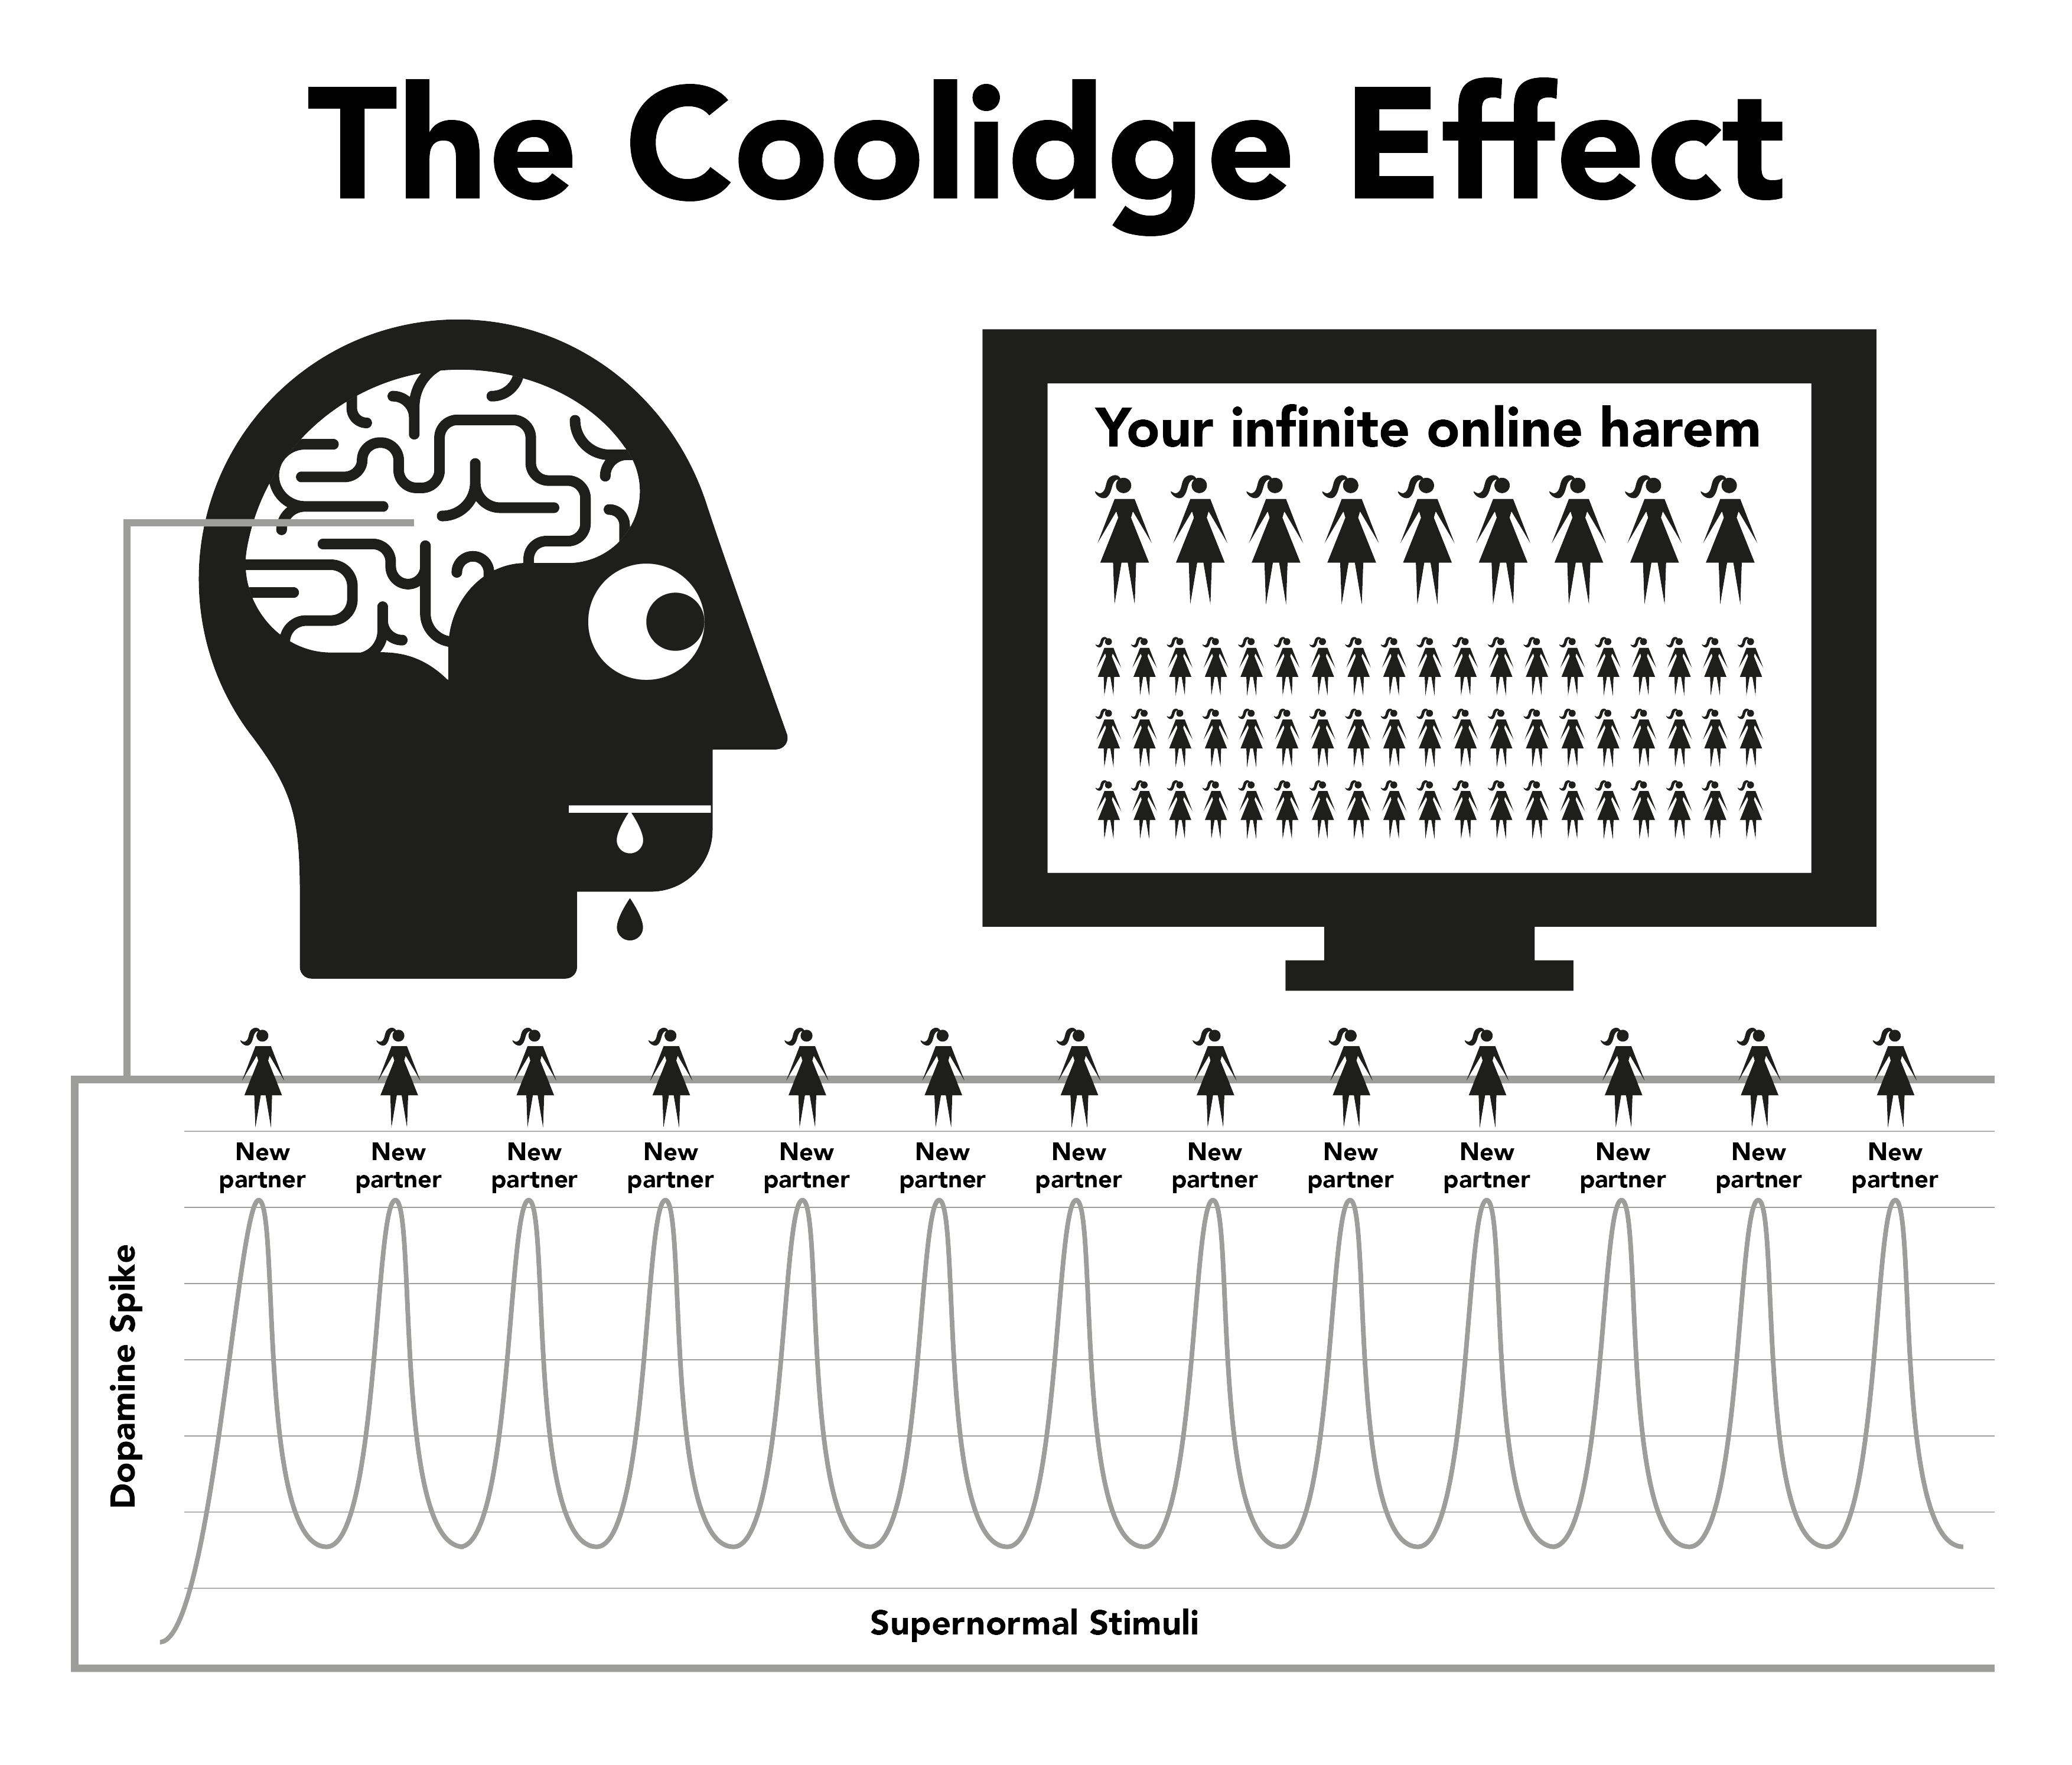
\includegraphics{images/coolidge.png}
(note - getting the background changed, sozzle. view the image manually or change the background to the light version in the `A' menu up the top)

\begin{quote}
\emph{``For in the dew of little things the heart finds it's morning and is refreshed''}

--- Kahlil Gibran
\end{quote}

A fleeting feeling of security is all that's needed to get through a rough spot in life, but will your desensitised brain be able to catch that drop of destresser that a non-user's brain is able to use?

Dopamine flooding acts like a quick acting drug, falling quickly and inducing withdrawal pangs. Many users have the illusion these pangs are the terrible trauma they suffer when trying or being forced to stop. In fact, they're primarily mental since the user is feeling deprived of their pleasure or prop.

\hypertarget{the-little-monster}{%
\section{The Little Monster}\label{the-little-monster}}

The actual chemical withdrawal from porn is so subtle that most users have lived and died without realising they're drug addicts. Many users have a fear of drugs, yet that's exactly what they are, drug addicts. Fortunately it's an easy drug to kick, but you first need to accept that you are, in fact, addicted. Withdrawal from porn doesn't cause any physical pain and is merely an empty, restless feeling of something missing, which is why many believe it's something to do with sexual desires. Prolonged, this feeling becomes nervousness, insecurity, agitation, low confidence and irritability. It's like hunger, for a poison.

Within seconds of engaging in a session, dopamine is supplied and the craving ends, resulting in a feeling of fulfillment as you whiz down the water slide. In the early days, withdrawal pangs and their subsequent relief are so slight we're unaware of them. When we become regular users, we believe it's because we've come to enjoy them or gotten into the 'habit'. The truth being that we're already hooked but don't realise it. The little monster is already in our brains, so every once and a while we take trips down the water slide to feed it.

All users begin seeking porn for irrational reasons. The \emph{only} reason anybody continues using porn, whether they're a casual or heavy user, is to feed that little monster. The whole conundrum is a series of cruel and confusing punishments, but perhaps the most pathetic aspect is the sense of enjoyment a user gets from a session, trying to get back to the sense of peace, tranquility and confidence their body had before becoming hooked in the first place.

\hypertarget{the-annoying-alarm}{%
\section{The Annoying Alarm}\label{the-annoying-alarm}}

You know that feeling when a neighbour's home alarm has been ringing all day - or some other minor persistent aggravation - then the noise suddenly stops and marvellous feelings of peace and tranquility wash over you? This isn't really peace, but the ending of an aggravation. Before starting the next session our bodies are complete, but then we begin forcing our brains to pump dopamine and when we're done and it begins to leave, we suffer withdrawal pangs. These aren't physical pain, merely an empty feeling. We aren't even aware it exists but it's like a dripping tap inside our bodies.

Our rational minds don't understand it, but they don't need to. All we know is that we want porn and when we masturbate the craving goes. However, the satisfaction is fleeting because in order to relieve the craving more porn is required. As soon as you orgasm, the craving starts again and the trap continues to hold you. A feedback loop, unless you break it!

The porn trap is similar to wearing tight shoes just to obtain the pleasure of taking them off. There are three primary reasons why users can't see it this way.

\begin{enumerate}
\def\labelenumi{\arabic{enumi}.}
\item
  From birth, we've been subjected to massive amounts of brainwashing telling us internet porn is simply another modern development that replaced the print version of porn. This fallacy is packaged with the truth that masturbation isn't harmful, so why shouldn't we believe them?
\item
  Because physical dopamine withdrawal involves no actual pain, merely an empty insecure feeling inseparable from hunger and normal stress, this feeling manifests into a porn session as those are the very times we tend to seek internet porn. We tend to regard this feeling as normal.
\item
  However, the primary reason users fail to see internet porn in it's true light is due to it working back to front. It's when you're \emph{not} consuming it that you suffer the empty feeling. Because the process of getting hooked is incredibly subtle and gradual in the early days, the empty feeling is regarded as normal and so isn't blamed on the previous session. The moment the browser is fired up and you begin your session, you get an immediate boost and become less nervous or more relaxed, so internet porn gets the credit.
\end{enumerate}

This 'back to front' reverse process makes all drugs difficult to kick. Imagine the state of panic of a heroin addict without any heroin; now picture the utter joy of when they can finally plunge a needle into their vein. Non-heroin addicts don't suffer that panicked feeling.

The heroin doesn't relieve the feeling, it causes it. Similarly, non-users don't suffer empty feelings of needing internet porn, or panic when they're offline. Non-users can't understand how users possibly obtain pleasure from two dimensional videos with muted sounds and abnormal body proportions. Eventually, users can't understand either.

We talk about internet porn being relaxing or satisfying, but how can you be satisfied unless you were dissatisfied in the first place? A non-user doesn't suffer from this unsatisfied state, completely relaxed after a no-sex date, while the user isn't until they've satisfied their 'little monster'.

\hypertarget{a-pleasure-or-a-crutch}{%
\section{A pleasure or a crutch?}\label{a-pleasure-or-a-crutch}}

An important reminder - the main reason that users find it difficult to quit is due to the belief they're giving up a genuine pleasure or crutch. It's essential to understand that you're giving up \emph{absolutely nothing} whatsoever. The best way to understand the subtleties of the porn trap is comparing it with eating. The habit of regular meals causes us to not feel hungry between, only aware of hunger if the meal is delayed. There's no physical pain, just an empty insecure feeling recognised as hunger. The process of satisfying our hunger is a very pleasant experience.

Pornography appears to be almost identical, but it's not. Like hunger, there's no physical pain and the reward mechanism behaves in similar ways, but it's this similarity to eating that tricks the user into believing there's a genuine pleasure or crutch. Although eating and porn appear to be very similar, in reality they're exact opposites.

\begin{itemize}
\item
  You eat to survive and energise your life, whereas porn dims and cuts down your mojo.
\item
  Food genuinely tastes good and eating is a genuinely pleasant experience that we enjoy throughout our lives. Porn involves self-sabotaging the happiness receptors and thus destroys your chances to cope and feel happy.
\item
  Eating doesn't create hunger and genuinely relieves it, whereas the first porn session starts the craving for dopamine and each subsequent session. Far from relieving it, it ensures suffering for the rest of your life.
\end{itemize}

Is eating a habit? If you think so, try breaking it completely! To describe eating as habit would be like describing breathing as a habit, both are essential for survival. It's true that people have the habit of satisfying their hunger at different times with varying types of food, but eating itself isn't habit. Neither is porn. The only reason a user fires up the browser is trying to end the empty feelings the previous session created, at different times with varying escalating genres.

On the internet, porn is frequently referred to as a habit and for convenience EasyPeasy also refers to the 'habit'. However, be constantly aware that porn isn't habit, it's \textbf{drug addiction!} When we start to use porn, we have to force ourselves to cope with it. Before we know it, we're escalating into increasingly bizarre and shocking porn. The thrill is in the hunting, not the killing, with dopamine rapidly leaving the body after orgasm, explaining why users want to 'edge' (delaying orgasm) through flicking between multiple browser windows and tabs.

\hypertarget{crossing-the-red-line}{%
\section{Crossing the red line}\label{crossing-the-red-line}}

As with any other drug, the body tends to develop immunity to the effects of the same old clips, our brain wanting more or something else. After short periods of watching the same clip it ceases to completely relieve the withdrawal pangs that the previous session created. There's a tug of war occurring in this porn paradise, you want to stay on the safe side of your 'red line' but your brain is asking you to click on the forbidden fruit clip.

You feel better after engaging in this porn session, but you're more nervous and less relaxed than someone who never started, even though you're living in a supposed porn paradise. This position is even more ridiculous than wearing tight shoes because as you go through life an ever increasing amount of discomfort remains after taking the shoes off. Because the users knows the little monster has to be fed, they themselves decide the time, tending to be on four types of occasions or a combination of them.\\
Boredom / Concentration - Two complete opposites!\\
Stress / Relaxation - Two complete opposites!

What magic drug can suddenly reverse the very effect it had minutes before? The truth is that porn neither relieves boredom and stress or promotes concentration and relaxation. If you think about it, what other types of occasions are there in our lives, bar sleep? If you have ideas of toning down to other types of 'realistic' or 'soft' genres of porn, please note the content of this book applies to all porn, print, webcams, pay-per-views, chat, live shows, etc. The human body is the most sophisticated object on the planet, but no species, even the lowest amoeba or worm, survives without knowing the difference between food and poison.

Through natural selection our minds and bodies developed techniques for rewarding actions that multiply and sustain humanity. They're not prepared for supernormal stimuli that are bigger, brighter and edgier than anything found in nature, even the most muted two dimensional image causes us to become aroused. But repeatably look at the same image and you won't be. In real life, checks and balances ensure you do something else but internet porn has no such limiter, causing you to spend your life in a virtual harem!

It's a fallacy that physically and mentally weak people become users, the lucky ones being those who found their first instance repulsive and are cured for life. Alternatively, they aren't mentally prepared to go through the severe learning process of fighting to get themselves hooked, fears of 'getting caught' or not being technical enough to operate browser privacy settings. Perhaps the most tragic part of the whole business relates to teenagers who are skilled in finding material and covering their tracks and start in increasing number.

Enjoying internet porn is an illusion. Jumping from genre to genre, merely keeping our novelty 'monkey' within the 'red line' of 'safe' porn genres in order to get our dopamine fix. Like heroin addicts, all they're really enjoying is the ritual of relieving those pangs.

\hypertarget{the-high-from-the-dance-around-the-red-line}{%
\section{The High From the Dance Around The Red Line}\label{the-high-from-the-dance-around-the-red-line}}

Even with the one clip that's lingered on, users constantly teach themselves to filter out the bad and ugly portions of porn clips. Even if it's solo, they still filter on the body parts that appeal to them the most. In fact, some take pleasure in this dance around the red line, finding excuses to declare they like the 'soft stuff' and are unaddicted to supernormal stimuli. But ask a user who believes they stick to a certain actor or genre, \emph{``If you cannot get your normal brand of porn and can only obtain an unsafe genre, do you stop masturbating?''}

No way! A user will masturbate to anything, escalating genres, differences in sex-orientation, look-alike performers, dangerous settings, shocking relationships, anything to sate the little monster. To begin with they taste awful, but given enough time you'll learn to enjoy them. Users will seek empty fulfillment after having real sex, after a long work day, fever, colds, flu, sore throats and even during admittance in hospitals.

Enjoyment has nothing to do with it, if sex is wanted, it makes no sense to be with your laptop. Some users find it alarming to realise they're drug addicts and believe this will make it even more difficult to stop. In fact, this is good news for two important reasons.

\begin{enumerate}
\def\labelenumi{\arabic{enumi}.}
\item
  The reason why most of continue using is because although we know the disadvantages far outweigh the advantages, we believe there's something in porn that we actually enjoy or that it acts like some sort of prop. We're under the illusion that after we stop using there will be a void, certain situations in our lives never being quite the same. In fact porn not only provides nothing, it only subtracts.
\item
  Although internet porn is the most powerful trigger for novelty and sex based dopamine flooding, because of the speed you become hooked you're never badly hooked. The actual withdrawal pangs are so mild that most users have lived and died without realising they've suffered them.
\end{enumerate}

Why is it then that many users find it so difficult to stop, going through months of torture and spending the rest of their lives pining for it at odd times? The answer is the second reason, brainwashing. The neurotransmitter addiction is easy to cope with, most users going for days without online porn on business trips or travel, unaffected by withdrawal pangs. Their little monster is safe in the knowledge you'll open your laptop as soon as you return to your hotel room. You can survive your obnoxious client and your megalomaniac manager, knowing the fix is there for your taking.

\hypertarget{the-smokers-analogy}{%
\section{The Smokers Analogy}\label{the-smokers-analogy}}

A good analogy is that of the cigarette smoker. If they went ten hours of the day without a cigarette they'd be tearing their hair out, but many smokers will buy a new car and refrain from smoking in it. Many will visit theatres, supermarkets, churches and being unable to smoke causes them no problems. Even on trains and airplanes there have been no riots. Smokers are almost pleased for someone or something to stop them smoking.

Users will automatically refrain from using internet porn in their parents' home during family gatherings and other events with little discomfort. In fact, most users have extended periods during which they abstain without effort. The neurological little monster is easy to cope with even when you're still addicted. There are millions of users who remain casual users all their lives and they're just as addicted as the heavy user. There are even heavy users who've kicked the addiction but have an occasional peek, greasing the water slide to be ridden down at the next dip in mood.

As said previously the actual porn addiction isn't the main problem, simply acting as a catalyst in keeping our minds confused over the real problem -- brainwashing. Don't think the bad effects of internet porn are exaggerated however, if anything they're sadly understated. Occasionally, rumours circulate that the neural pathways created are there for life, with the right mix of chance and stimulus sending you down the life ruining water slide again, but these are untrue. Our brains and bodies are miraculous machines, recovering within a matter of weeks.

It's never too late to stop! A quick browse of online communities will show you people of all ages rebooting their (and their partners) lives. As with anything humans do some take it to the next level, practicing semen retention, Karezza and through differentiation of the sensory and propagative sides of sex make their partners happier than ever before.

It may be of consolation to lifelong and heavy users that it's just as easy for them to stop as casual users, and in a peculiar way it's easier. The further it drags you down, the greater the relief. When I stopped I went straight to \emph{zero} and didn't have one bad pang. In fact, the process was actually enjoyable even during the withdrawal period.

But first, we must remove the brainwashing.

\hypertarget{brainwashing}{%
\chapter{Brainwashing}\label{brainwashing}}

This is the second reason we start using. Understanding this brainwashing fully required us to first examine the powerful effects of supernormal stimulus. Our brains simply aren't prepared for the creation of an 'online harem', allowing us to flick between more potential mates in fifteen minutes than our ancestors had in several lifetimes.

There's been much misguided advice in the past, an example being that masturbation leads to blindness. This, along with other scare tactics, clearly over did it. Misconceptions such as these were right to be overthrown by science. But the baby has been thrown out with the bath water; from our earliest years our subconscious minds are bombarded with sexual messages and imagery, magazines and advertisements loaded with innuendo. Some pop videos are extremely suggestive, but don't despair, make it a game to identify what components they're using -- is it shock value, novelty, colour, size, taboo, etc. Such a game can even be taught to pre-teens as a way to educate them.

At it's core, the message is \emph{``The most precious thing on this earth, my last thought and action, will be orgasm.''} Is this exaggeration? Watch any TV or movie plot and you'll see the mix up of the sensory (touch, smell, voice) and the propagative (orgasmic) parts of sex. The impact of this doesn't register on our conscious, but the subconscious has time to absorb it.

\hypertarget{scientific-reasoning}{%
\section{Scientific reasoning}\label{scientific-reasoning}}

There's publicity the other way, sexual dysfunction scares, loss of motivation, preferring virtual porn to real girls, YourBrainOnPorn and various internet subcultures, but these movements don't actually stop people from using. Logically speaking they should, but the simple fact is they don't. Even the health risks listed from peer reviewed studies on YourBrainOnPorn aren't enough to stop an adolescent from starting.

Ironically, the most powerful force in this confusion is the user themselves. It's a fallacy that users are weak-willed or physically weak people. You have to be physically strong in order to cope with an addiction after you know it exists. Perhaps the most painful aspect is that they place themselves as unsuccessful losers and insufferable introverts. It's likely that a friend could be more interesting in person if they hadn't put themselves down for seeking self-pleasure.

\begin{figure}
\centering
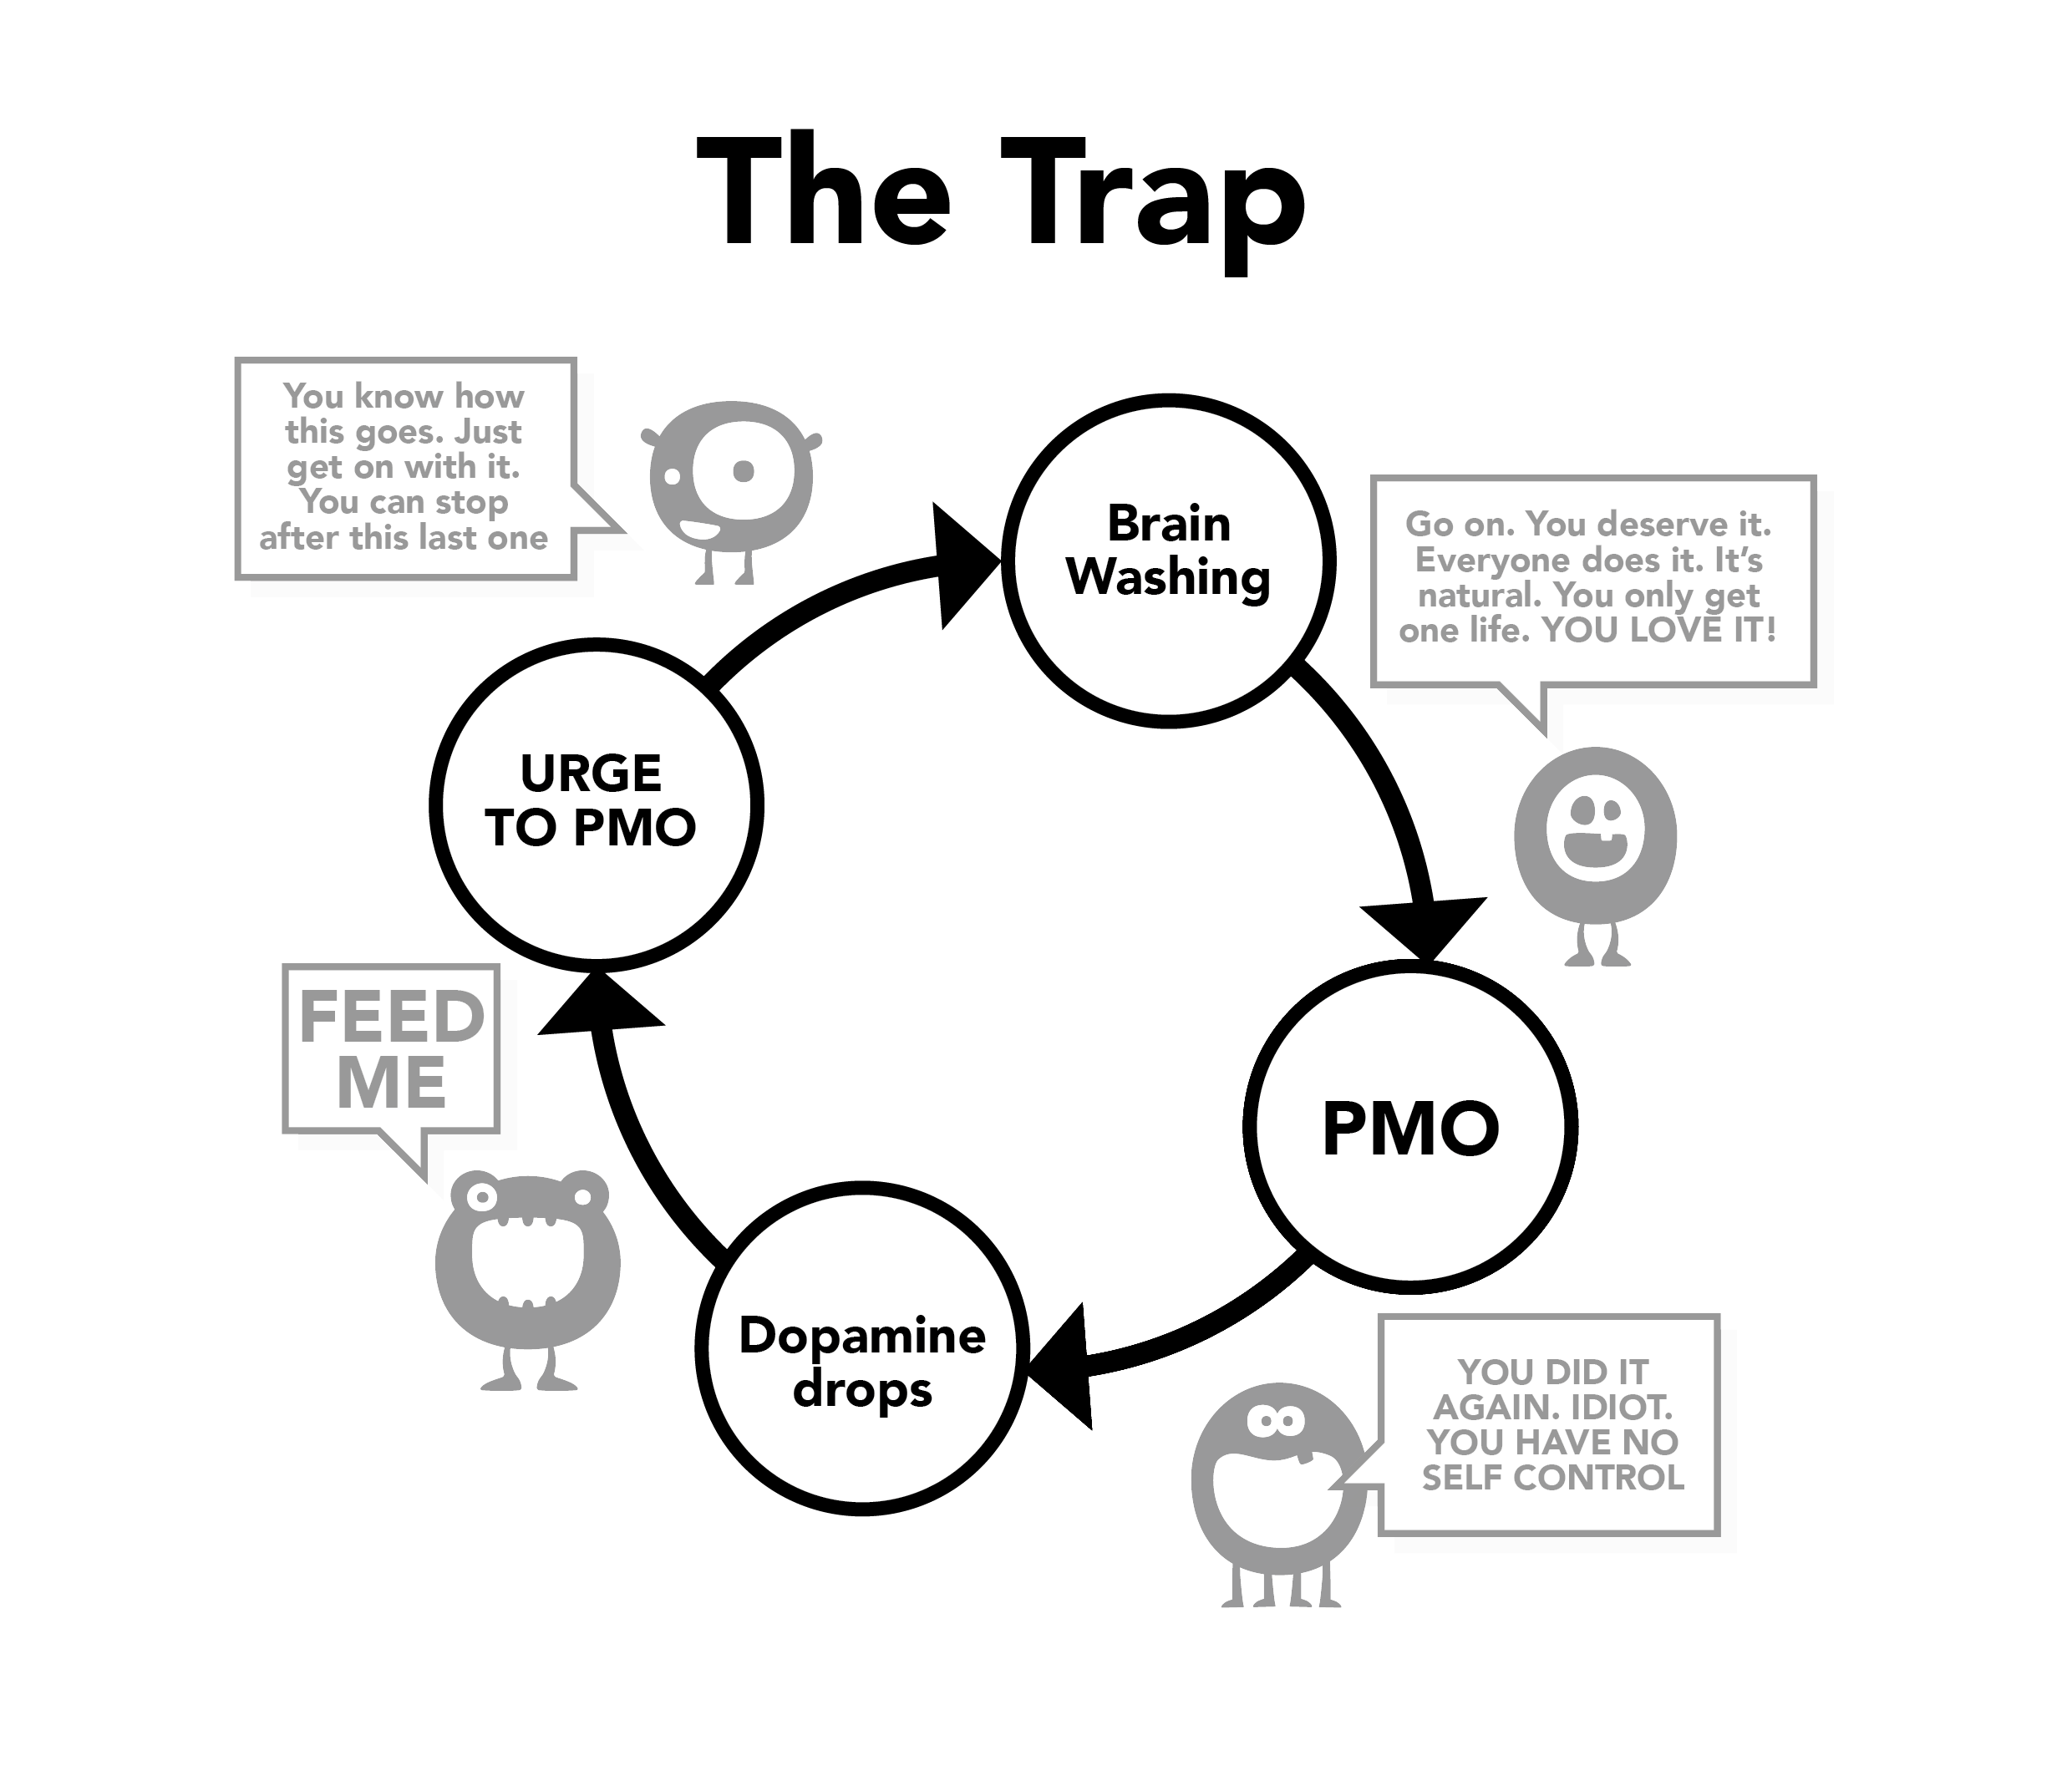
\includegraphics{images/trap.png}
\caption{The Pornography Trap}
\end{figure}

\hypertarget{the-willpower-method}{%
\section{The Willpower Method}\label{the-willpower-method}}

Users quitting using the willpower method blame their own lack of willpower and ruin their peace and happiness. It's one thing to fail in self-discipline and another to self-loathe. After all, there's no law that requires you to be hard all the time before sex, properly aroused and able to satisfy your partner. We're working on an addiction, not a habit and at no point do you argue with yourself to stop a habit like golfing, but to do the same with porn addiction is normalised, why?

Constant exposure to a supernormal stimulus rewires your brain, so building a resistance to this brainwashing is critical, as if buying a car from a second hand car dealer - nodding politely but not believing a word the man is saying. So don't believe that you must have as much sex as you can, all of it being exceptionally good, using porn in it's absence.

Don't play the safe porn game either, your little monster invented that game to lure you. Is amateur porn certified by some authority? Porn sites gather data from their users and use it to cater to their needs, if they see a uptick in a certain category they'll focus on it and get content out ASAP. Don't be fooled by educational intent or 'safe' female marketed clips. Start asking yourself: \emph{``Why am I doing it? Do I really need to?''}

\textbf{No, of course you don't!}

Most users swear that they only watch static and soft porn and therefore are fine, when in actuality they're straining at the leash, fighting with their willpower to resist temptations. If done too often and for too long, this depletes their willpower considerably and so they begin failing in other life projects where willpower is of great value, like exercise, dieting, etc. Failure in these areas makes them feel miserable and guilty, cascading and kicking them back into pornography. If this isn't done, they'll vent their anger and depression onto loved ones.

Once you become addicted to internet porn, the brainwashing is increased. Your subconscious mind knows the little monster has to be fed, blocking everything else. It's fear that keeps people from quitting, fear of that empty, insecure feeling they get when they stop flooding their brains with dopamine. Just because you're unaware of it doesn't mean it's not there. You don't have to understand it any more than a cat needs to understand where the hot water pipes are, the cat just knows that if it sits in a certain spot it feels warm.

\hypertarget{passivity}{%
\section{Passivity}\label{passivity}}

The passivity of our minds and dependence on authority leading to brainwashing is the primary difficulty of giving up porn. Our upbringing in society, reinforced by the brainwashing of our own addiction and combined with the most powerful - our friends, relatives and colleagues. The phrase 'giving up' is a classic example of the brainwashing, implying genuine sacrifice. The beautiful truth is there's nothing to give up; on the contrary, you'll be freeing yourself from a terrible disease and achieving marvellous positive gains. We'll begin removing this brainwashing now, starting with no longer referring to 'giving up' but to stopping, quitting or perhaps the true position, \textbf{escaping!}

The only thing that persuades us to use initially is other people doing it, feeling that we're missing out. We work hard to become hooked, yet never find what they've been missing. Every time we see another clip it reassures us there must be something in it, otherwise people wouldn't be doing it and the business wouldn't be so big. Even when they kick the habit, the ex-user feels they're being deprived when a discussion on a sexy entertainer, singer or even a porn star comes up during parties or social functions. \emph{``They must be good if all my friends talk about them, right? Do they have free pictures online?''} They feel safe, they'll just have one peek tonight and before they know it, they're hooked again.

The brainwashing is extremely powerful and you need to be aware of its effects. Technology continues to grow and the future will bring exponentially faster sites and access methods. The porn industry is investing millions in virtual reality so that it will become the next best thing. We don't know where we're going, unequipped to deal with present technology or what is to come.

We're about to remove this brainwashing, it isn't the non-user who's being deprived but the user who is forfeiting a lifetime of:

\begin{itemize}
\item
  Health
\item
  Energy
\item
  Wealth
\item
  Peace of mind
\item
  Confidence
\item
  Courage
\item
  Self-respect
\item
  Happiness
\item
  Freedom
\end{itemize}

What do they gain from these considerable sacrifices? \textbf{ABSOLUTELY NOTHING}, apart from the illusion of trying to get back to the state of peace, tranquillity and confidence that the non-user always enjoys.

\hypertarget{withdrawal-pangs}{%
\section{Withdrawal Pangs}\label{withdrawal-pangs}}

As explained earlier, users believe they use porn for enjoyment, relaxation or some sort of education. The actual reason is relief of withdrawal pangs. Our subconscious mind begins to learn that internet porn and masturbation at certain times tends to be pleasurable. As we become increasingly hooked on the drug, the greater the need to relieve the withdrawal pangs becomes and the further the subtle trap drags you down. This process happens so slowly that you aren't even aware of it, most young users don't realise they're addicted until attempting to stop and even then, many won't admit it.

Take this conversation a therapist had with hundreds of teenagers:

\textbf{Therapist:} ``\emph{You realise that internet porn is a drug and the only reason why you're using is that you cannot stop.}''
\textbf{Patient:} ``\emph{Nonsense! I enjoy it, if I didn't, I would stop.}''
\textbf{Therapist:} ``\emph{Just stop for a week to prove to me you can if you want to.}''
\textbf{Patient:} ``\emph{No need, I enjoy it. If I wanted to stop, I would.}''
\textbf{Therapist:} ``\emph{Just stop for a week to prove to yourself you aren't hooked.}''
\textbf{Patient:} "\emph{What's the point? I enjoy it."}

As already stated, users tend to relieve their withdrawal pangs at times of stress, boredom, concentration or combinations of these. In the following chapters, we'll target these aspects of brainwashing.

\hypertarget{brainwashing-aspects}{%
\chapter{Brainwashing Aspects}\label{brainwashing-aspects}}

The porn trap's big monster is bred through the culmination of many aspects, including societal forces, media portrayals, peers and the user's own internal narrative. Failure to deconstruct these fallacies whilst using the willpower method eventually leads to feelings of deprivation, leading the user back into the trap. Deconstruction of the imagined value of porn is crucial for success and allows you to see where you're being robbed!

Of importance to note is the link between brainwashing and fear. It's fear of feeling \textbf{\emph{future withdrawal pangs}} that create the pangs. Fear is the pang itself. Think when you've had withdrawal symptoms such as sweaty palms, shortness of breath, sleeping problems and inability to think straight. Now think of similar situations when you've had those feelings: job interviews, nerves around an attractive person, public speaking, etc. These are the same anxious feelings the fear causes. Simply put, how can a physical drug still hook people months after stopping? It must be mentally, correct?

\hypertarget{stress}{%
\section{Stress}\label{stress}}

Not only great tragedies in life, but also minor stresses drive users into the forbidden `unsafe' area previously excluded. Stresses include socialising, phone calls, anxieties of the housewife with young children, and many others. Let's take phone calls as an example, particularly for a businessperson. Most calls aren't from satisfied customers or your boss congratulating you, there's some sort of aggravation. Coming home to mundane family life of kids screaming and their partner's emotional demands causes the user - if they aren't already doing so - to fantasise the relief of porn promised that night. They unconsciously suffer withdrawal pangs, destressors weakened and unprepared for additional aggravation. Partially relieving the pangs at the same time as normal stress, the total is reduced and the user gets a temporary boost. The boost isn't an illusion, the user does genuinely feel better than before, but they're more tense than they would be as a non-user.

The following example isn't designed to shock you, EasyPeasy promises no such treatment, but is to emphasise that porn destroys your nerves rather than relaxing them.

Try to imagine getting to the stage where you're unable to be aroused, even with a very sexy and attractive partner. For a moment, pause and try to visualise life where a very lovely and charming person has to compete and fail with the virtual porn stars occupying your 'harem' to get your attention. Imagine the frame of mind of a person who, when issued with that warning, continues using and dies without ever having real sex with this charming and willing partner. It's easy to dismiss these people as weirdos, but stories like these aren't fakes, this is what the awful novelty of the porn drug does to your brain. The more you go through life, the more courage is sapped and the more you're deluded into believing porn is doing the opposite.

Have you ever been overtaken by panic when out of the blue the WiFi stops working or is too slow? Non-users don't suffer from it, as internet porn \emph{causes} that feeling. As you go through life, it systematically destroys your nerve and courage, leaving DeltaFosB to form powerful neural water slides in its wake, progressively destroying your ability to say no. By the stage where virility has been killed, the user believes porn is their new partner and is unable to face life without it.

\emph{Internet porn isn't relieving your nerves, it's slowly destroying them}. One of the great gains of breaking the addiction is the return of your natural confidence and self assurance.

There's no need to self-rate based on your ability to satisfy a partner, this isn't freedom. But this freedom cannot be obtained by continuing to grease the dopamine water slide in ways that undercut your happiness and libido by repeating the same destructive behaviour.

\hypertarget{boredom}{%
\section{Boredom}\label{boredom}}

If you're like many people, as soon as you climb into bed you're already on your favorite porn site, probably already forgetting until reminded. It's become second nature. Similarly, porn relieving boredom is another fallacy because boredom is a frame of mind; occurring when you've been deprived for a long time or are trying to cut down.

The actual situation is this, when you're addicted to the supernormal pull of internet porn and then try to abstain, it feels like there's something missing. If you have something to occupy your mind that isn't stressful, you can go for long periods of time without being bothered by the absence of the drug. However, when you're bored there's nothing to take your mind off it, so you feed the monster. When you're indulging yourself and not trying to stop or cut down, even firing up private browsing becomes subconscious. This ritual is automatic; if the user tries to remember sessions during the last week, they're only able to remember a small proportion of them, like the very last one or the session after a long abstinence.

The truth being that porn increases boredom indirectly because orgasms make you feel lethargic and instead of undertaking an energetic activity, users tend to prefer lounging around, bored and relieving their withdrawal pangs. Countering the brainwashing is important because users tend to view porn when bored, our brains wired to interpret porn as interesting. Similarly, we've also been brainwashed into believing sex - even bad sex - aids relaxation. It's a fact that when sad or under stress, couples want to have sex. In the absence of discrimination between sensory and propagative sex, watch how quickly you want to get away from each other after the mandatory orgasm is achieved. If the couple had just decided to hug, speak or cuddle and go to sleep, they'd have felt relieved.

\hypertarget{concentration}{%
\section{Concentration}\label{concentration}}

Masturbation and sex don't help concentration, when you're trying to concentrate you automatically try and avoid distractions. Therefore, when a user wants to concentrate, they don't even think, automatically opening the browser, feeding the little monster and partially ending the craving. Getting on with the matter at hand, already forgetting they've viewed porn. After years of dopamine flooding the neurological changes affect abilities such as accessing information, planning and impulse control.

You're also driven to provide novelty for the next session as the same stuff no longer generates enough dopamine and opioids. So you'll have to roam the internet streets for novelty, fighting the pull to cross the line towards shocking material, this in turn generating more stress and leaving you unfulfilled after finishing.

Concentration is also adversely affected due to dopamine receptors being culled due to natural tolerance to the large surges, reducing the benefit of smaller dopamine boosts from natural destressors. Your concentration and inspiration will be greatly boosted as this process is reduced. For many, it's the concentration aspect that prevents them from succeeding with the willpower method, they could put up with the irritability and bad temper, but the failure to concentrate on something difficult once their crutch is removed ruins many.

Loss of concentration that users suffer when trying to escape isn't due to the absence of sex, let alone porn. You have mental blocks when you're addicted to something and when you have a mental block, what do you do? You fire up the browser - which doesn't cure the block - so then what do you do? You do what you have to do, getting on with it just as non-users do.

When you're a user nothing is blamed on the cause, users never have \emph{sexual dysfunction}, just occasional down time. The moment you stop using, everything that goes wrong is blamed on the reason you stopped. Now when you have a mental block, instead of just getting on with it, you begin to say ``\emph{If only I could check my harem now, it would solve all my problems}''. You then begin to question your decision to quit and escape from the slavery.

If you believe that porn is a genuine aid to concentration, worrying about it will guarantee that you'll be unable to concentrate. Doubt, not the physical withdrawal pangs creates the problem. Always remember, it's the user who suffers pangs, not non-users.

\hypertarget{relaxation}{%
\section{Relaxation}\label{relaxation}}

Most users think that porn helps them to relax. It doesn't. The frantic search to get the fix in those 'dark alleys of the internet' and the internal struggle of straining at the leash to cross the red line certainly doesn't sound like a very relaxing activity.

As night rolls in after a trip to a new place or a long day, we sit down to relax, relieving our hunger, thirst and are completely satisfied. The user is not, as they have another hunger to satisfy. Users think of porn as the icing on the cake, but in actuality it's the 'little monster' that needs feeding. The truth is that the addict can never be completely relaxed and going through life it gets exponentially worse. Take one online comment from an ex-user:

\begin{quote}
``\emph{I really believed that I had an evil demon in my make up, I now know that I had, however it wasn't some inherent flaw in my character but the little internet porn monster that was creating the problem. During those times I thought I had all the problems in the world, but when I look back on my life I wonder where all the great stress was. In everything else in my life I was in control, only thing controlling me was porn slavery. The sad thing is that even today I can't convince my children that it was the slavery that caused me to be so irritable.}''
\end{quote}

Every time I hear porn addicts trying to justify their addiction the message is, ``\emph{Oh it helps me to relax.}'' Take this online account of a single dad whose six year old son wanted to share his bed in the night after a scary movie, but the dad would refuse so that he could have his session and edge for hours.

Here's another smoking analogy, a couple of years ago adoption authorities threatened to prevent smokers from adopting children. A man rang up, irate. ``\emph{You're completely wrong}'', he said, ``\emph{I can remember when I was a child, if I had a contentious matter to raise with my mother, I would wait until she lit a cigarette because she was more relaxed then.}'' Why couldn't the man talk to his mother when she wasn't smoking a cigarette?

Why are some users so stressed when they're not getting their fix, even after real sex? One story online details a man working in the advertising field having 9s and 10s open for dates at any time, but lost interest in taking them out for dinner as internet porn was far easier, involved no restaurant spending and had no possibility of a 'no' from his date at the end of an evening. Why be bothered when his little monster keeps him craving the low risk, high reward scheme at his fingertips upon reaching home?

Why are non-users completely relaxed then? Why are users not able to relax without a fix for a day or two? Read about the experience of a user taking the abstinence oath and quitting and you'll notice the struggle with temptations, clearly not relaxed at all when no longer allowed to have the 'only pleasure' they are 'entitled to enjoy'. They've forgotten what it's like to be completely relaxed. Porn can be likened to a fly being caught in a pitcher plant, to begin with the fly is eating the nectar but at some imperceptible stage the plant begins to eat the fly.

Isn't it time you climbed out of the plant?

\hypertarget{energy}{%
\section{Energy}\label{energy}}

Most users are aware of the progressive effects of porn's novelty and escalation seeking has on their brains reward and sexual systems. However, they aren't aware of the effect it has on their energy level.

One of the porn trap's subtleties is that the effects it has upon us both physically and mentally, happen so gradually and imperceptibly that we aren't aware of them and instead regard them as normal. The effect is similar to that of bad eating habits, we look at people who are grossly overweight and wonder how they could have possibly allowed themselves to reach that state. But suppose that it happened overnight - you went to bed trim, rippling with muscles and not an ounce of fat on your body - and awoke to find yourself fat, bloated and pot-bellied. Instead of waking up feeling fully rested and full of energy, you feel miserable, lethargic, and barely able to open your eyes.

You'd be panic stricken, wondering what awful disease you had contracted overnight, and yet the disease is exactly the same. The fact it took you twenty years to arrive there is irrelevant. Porn is the same, if it was possible to immediately transfer your mind and body to give you a direct comparison on how you'd feel having stopped porn for just three weeks, that's all that would be required to convince you. Asking if you'd really feel this good or what it really amounts to, ``\emph{Had I really sunk that low?}'' You wouldn't just feel healthier with more energy but sprouting far more confidence and a heightened ability to concentrate.

Lack of energy, tiredness and everything related to it is nicely swept under the rug of 'getting older'. Friends and colleagues who also live sedentary lifestyles further compound the normalisation of this behaviour. The belief that energy is the exclusive prerogative of children and teenagers and that old age begins in your twenties is another symptom of the brainwashing, as is being unaware of eating and exercise habits as a result of the compounding effects of dopamine desensitisation.

Shortly after stopping porn, the foggy and muggy feeling will leave you. The point being, with porn you're always debiting your energy and in that process, tampering with the chemistry of your limbic system. Unlike quitting smoking, where the return of your physical and mental health is only gradual, quitting porn gives you excellent results from day one. Killing the 'little monster' and closing the water slides takes a little bit of time, but recovering your reward centre is nothing like the slow slide into the pit. If you're going through the trauma of the willpower method, any health or energy gains will be obliterated by the depression you'll be going through. Unfortunately, it's not possible for EasyPeasy to immediately transfer you into your mind in three weeks time, but you can! You know instinctively that what you're being told is correct, all you need to do is \textbf{use your imagination!}

\hypertarget{social-night-sessions}{%
\section{Social Night Sessions}\label{social-night-sessions}}

This is misinformation that seems to make sense, but doesn't. In order to control your appetite, will you eat at home before leaving to go to a restaurant or party? This is what you're doing with sessions before social nights, looking tired and not up to your best. The widespread adoption of pick-up techniques has introduced pressure to perform, pick-up and score. Attempting to drown your butterflies with porn and substances will only make the problem worse in the long run. Personally, I like a bit of anxiety to keep me focused and engaged and tiring yourself out mentally and physically with orgasm isn't going to help.

Social night porn is occasioned by two or more of our usual reasons for pleasure/prop seeking, social functions at their core are both stressful and relaxing. This might appear to be a contradiction but any form of socialisation can be stressful - even with friends - wanting to be yourself and completely relaxed. There's many occasions that have multiple factors present at any one time, take driving as an example, since after all, your life is at stake. Stressful, with concentration required for a sustained period of time. You need not be aware of these factors, your subconscious already receiving the message. By the same token, finding yourself stuck in traffic jams or bored on long highway drives, perhaps promising yourself a session upon reaching home.

Another good example is going on a first date, your mind throwing out questions about the person you're about to meet. Then after meeting the person in the flesh, if enthusiasm starts to fade you'll start to feel too relaxed, then guilty for feeling this way. The tug of war has started, ``\emph{I want sex or get me out of here ASAP}'', priming you for post date porn.

Even if the date went well and hours later you're back at their place, no matter which way it goes you won't be satisfied if your only goal is seeking orgasm. At other times you drive home alone, your only thought being your online harem instead of congratulating yourself for your efforts. You can bet that someone in this position will have a session upon reaching home, and it's often after nights like these - waking to feel uneasy emptiness - are the ones we'll miss the most when contemplating stopping porn. We think that life will never be quite as enjoyable again. In fact, it's the same principle at work: the sessions simply provide relief from the withdrawal pangs, at some times having greater needs than others, greasing the water slide for the next cue.

Make this clear - it's not internet porn and harem dwellers that are special, it's the occasion. Once the need for porn is removed, such occasions will become more enjoyable and stressful situations less stressful.

\begin{figure}
\centering
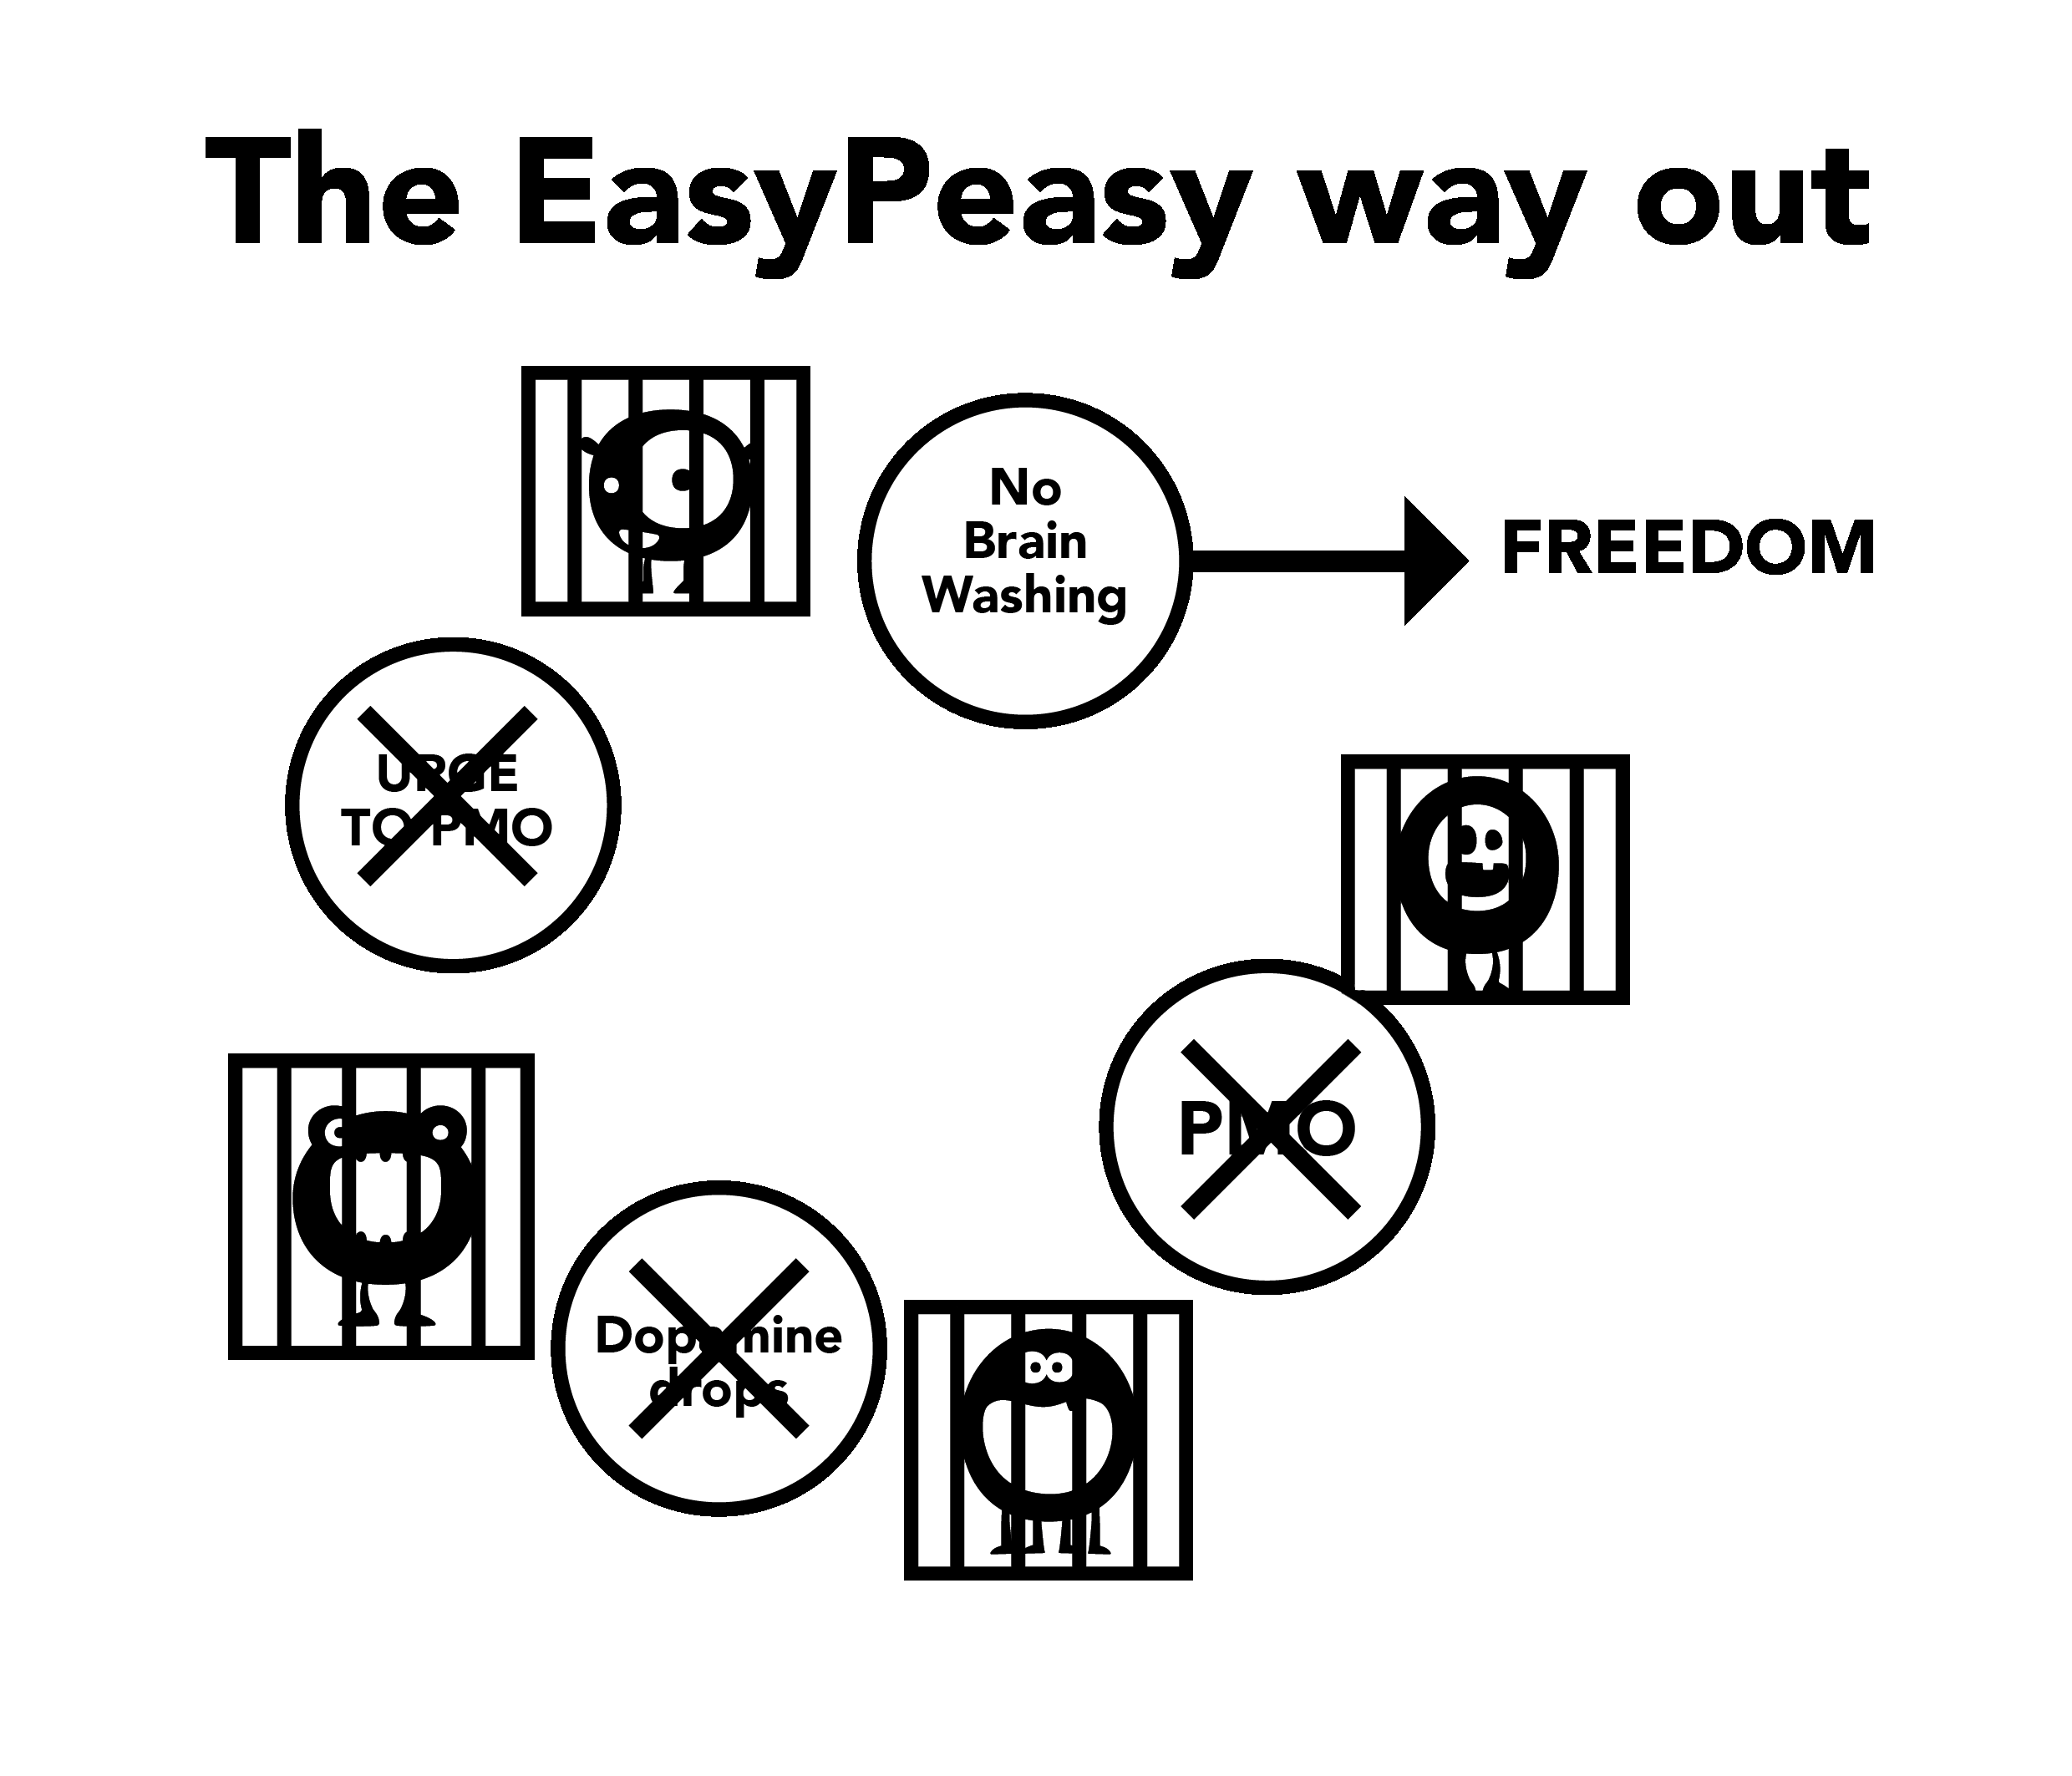
\includegraphics{images/trap-resolved.png}
\caption{Removing the brainwashing graphic}
\end{figure}

\hypertarget{what-am-i-giving-up}{%
\chapter{What am I giving up?}\label{what-am-i-giving-up}}

\textbf{Absolutely nothing!} Porn is difficult to give up because of fear we're being deprived of our pleasure or prop. The fear that certain pleasant situations will never be quite the same again. Fear of being unable to cope with stressful situations. In other words, it's the effects of brainwashing deluding us into believing that sex - and by extension orgasm - is a must for all human beings. Even further, it's the belief there's something inherent in internet porn that we need, and that when we stop using we will be denying ourselves and creating a void.

Make this clear in your mind: Porn doesn't fill a void, it creates one!

Our bodies are the most sophisticated objects on the planet. Whether you believe in intelligent design, natural selection or a combination of both, our bodies are thousands of times more effective than man! We're unable to create the smallest living cell or the miracles of eyesight, reproduction and various interlinked systems present in our bodies or brains. If this creator or process had intended us to handle supernormal stimulus, we'd have been provided with different reward systems. Our bodies are provided with fail-safe warning devices and we ignore these at our peril.

\hypertarget{theres-nothing-to-give-up}{%
\section{There's nothing to give up}\label{theres-nothing-to-give-up}}

Once you purge the little monster from your body and the brainwashing (the big monster) from your mind, you'll neither want to masturbate often or use internet porn for it. There are many knowns and unknowns when it comes to porn addiction, with many in the medical community having no concept of questioning or determining someone as a porn addict. A lot of reported symptoms are wrongly tagged under other causes. It's not that users are generally stupid people, it's just that they're miserable without porn. Caught between the devil and the deep blue sea, abstaining and being miserable because they cannot use porn or miserable because they're guilty and begin despising themselves because of it. When they get symptoms such as lower back pain or PIED, their minds are torn between accepting responsibility and looking the other way.

Another smoker analogy, all of us have seen smokers who develop excuses to sneak off for a crafty puff and we see the true addiction in action. Addicts don't do this for enjoyment, instead they do it because they're miserable without it.

For many their first sexual experience ended in an orgasm, so they acquire the belief they can't enjoy sex without one. For men, porn is marketed as an aid towards sex, sometimes even as an education in confidence during the act. This is nonsense, the conditioning of supernormal stimulus only succeeds in bringing it down.

Not only is there nothing to give up but massive positive gains to be had. When users contemplate quitting, they tend to concentrate on health and virility. These are valid and important reasons, but I personally believe the greatest gains are psychological:

\begin{itemize}
\item
  The return of your confidence and courage.
\item
  Freedom from slavery.
\item
  No longer having awful black shadows at the back of your mind and despising yourself.
\end{itemize}

\hypertarget{void-the-void-the-beautiful-void}{%
\section{Void, the void, the beautiful void!}\label{void-the-void-the-beautiful-void}}

Imagine having a cold sore on your face, so you go to the pharmacist and he gives you a free ointment to try. You put the ointment on and it disappears immediately. A week later it reappears, so you go back to the pharmacist and ask if they have any more ointment. The pharmacist says \emph{``Sure, keep the tube, you might need it later.''}

You apply the ointment and hey presto, the sore disappears once again. But every time the sore returns, it gets larger and more painful, with the interval getting shorter and shorter. Eventually, the sore covers your whole face and is excruciatingly painful, and it's returning every half hour. You know the ointment will remove it temporarily, but you're very worried. Will the sore eventually spread over your whole body? Will the interval disappear completely? You go to your doctor and they can't cure it, so you try other things but nothing helps apart from the ointment.

By now you're completely dependent on the ointment, never going out without ensuring that you have a tube with you. If you go abroad, making sure you take several tubes with you. In addition to your worries about your health, the pharmacist is charging you a hundred dollars a tube. You have no choice but to pay up.

You stumble across an article discussing this and find out it isn't just happening to you, many people are suffering from the same problem. In fact, the medical community has discovered that the ointment doesn't actually cure the sore, instead only taking it beneath the surface of the skin. It's the ointment that caused the sore to grow so all you have to do to get rid of the sore is to stop using the ointment and it'll disappear in due course.

Would you continue to use the ointment? Would it take willpower to not use the ointment? If you didn't believe the article there might be a few days of apprehension, but once you realised the sore was beginning to get better, the need or desire to use the ointment would go. Would you be miserable? Of course you wouldn't! You had an awful problem which you thought was incurable but now you've found the solution. Even if it took a year for the sore to go away, each day as it improved you'd think about how marvellous you felt. This is the magic of quitting porn.

The sore isn't the body pains, lack of normal lust, flagging arousal, fading penetration, wasted time spent on two-dimensional images, feelings of infringement on entitlement, despising the people who caught you or even worse, despising yourself. These are all in addition to the sore.

The sore makes us close our minds to all these things, it's that panic feeling of wanting a fix. Non-users don't suffer from that feeling. The worst thing we ever suffer is fear, the greatest gain being rid of that fear. It's caused by your first session, further strengthened and caused by each subsequent one.

Some users are 'happy', blinded by their cunning little monsters and so go through this same nightmare, putting up phony arguments to try and justify their stupidity.

\emph{It's so nice to be free!}

\hypertarget{saving-time}{%
\chapter{Saving Time}\label{saving-time}}

Usually when users try stopping, the main reasons given are health, religion and partner stigma. Part of the brainwashing of this awful drug is the sheer slavery of it, man has fought hard to abolish slavery in many parts of the world - yet the user spends life suffering self-imposed slavery. They're oblivious to the fact that when they're allowed to use porn they wish they were a non-user. The only time that porn becomes precious is when we're 'trying' to cut down or abstain, or when abstinence is forced on us.

It cannot be repeated often enough that brainwashing makes it difficult to stop porn, the more we dispel before we start, the easier you'll find it to achieve your goal. Confirmed users, who don't believe that porn has any negative effect on their health (porn induced erectile dysfunction, hypofrontality, etc.) and aren't having a mental tug of war are typically younger or single with an occasional sex partner. Thus, the internal feedback is lost due to the nature of their youth or is too infrequent to be observed and registered.

A better argument for a younger user is the time spent, rather saying ``\emph{I can't believe you aren't worried about the time you are spending.}'' Generally their eyes light up, feeling disadvantaged if attacked on health grounds or social stigma, but on time\ldots{}\\
``\emph{Oh, I can afford it. It's only x hours per week and I think it's worth it, it's my only vice of pleasure.}''

``\emph{I still can't believe you're not worried. Let's assume a half hour daily average which includes the physical drain of dopamine withdrawals, you're spending approximately a full working day every fortnight. I'm sure you'd agree that half an hour a day is a very conservative estimate. Have you thought about how much time you'll spend in your lifetime? What are you doing in that time? Developing real relationships? No, your favorite porn star doesn't have sympathy for you, just because you spent so much time on their videos -- you're throwing time away! Not only that, you're actually using that time to ruin your physical health, destroying your nerves and confidence in order to suffer a lifetime of slavery, pain, melancholy and peevishness. Surely that must worry you, right?}''

It's apparent at this point - especially with younger users - that they've never considered it a lifetime addiction. Occasionally, they work out the time they waste in a week and that's alarming enough. Very occasionally, and only when they think of stopping, they'll estimate what they spend in a year which is frightening - but over a lifetime is unthinkable. However, because we're in an argument the confirmed user will impulsively say, \emph{``I can afford it, it's only so much a week''}, pulling an encyclopedia salesman routine on themselves.

Would you refuse a job offer which pays your current annual salary and also gives you a month off every year? Any user would sign in a heartbeat and would get busy finding holiday deals to exotic locations. Figuring out how to spend a full month with no work would be the biggest problem to solve. In every discussion with a confirmed user (and please bear in mind that's not someone like yourself who plans to stop) nobody has ever taken me up on that offer. Why not?

Often at this point, a confirmed user will say, ``\emph{Look, I'm not really worried about the money aspect.}'' If you're thinking along those lines ask yourself why you aren't worried. Why in other aspects of your life will you go to great deals of trouble to save a few dollars here and there, but spend thousands killing your happiness and hanging the expense?

Every other decision you make in your life will be the result of an analytical process of weighing up advantages and disadvantages to arrive at a rational decision. It may be the wrong decision, but it'll be the result of rational deduction. Whenever any user weighs up the pros and cons of using internet porn, the answer is a dozen times over, \textbf{``STOP USING! YOU'RE A MUG!''} Therefore, all users are using not because they want or decide to, but because they can't stop. They \textbf{\emph{have}} to use porn, and so brainwash themselves, keeping their heads in the sand.

Confirmed users should keep in mind that the situation will only get exponentially worse, with more studies coming out and more people talking about the ill effects of internet porn. Today, it's non-medical people discussing the effects, tomorrow it'll be on your doctor's list of diagnostic tests. Gone are the days where the user can hide 'downtime' behind work stress in their sex life, your partner is going to ask why you're on your laptop late at night. The poor user - already feeling wretched - now wants the ground to open up and swallow them.

The strange thing is that many people would pay good money for gym memberships and personal trainers to build muscles and look sculpted, many in their imaginary (and real) desperation turning to treatments such as boosting testosterone with dubious and dangerous side effects. Yet there are many people in this group who would benefit from stopping a practice systematically destroying their brain's natural relaxation systems.

This is because they're still thinking with the brainwashed mind of the user. Wipe the sand out of your eyes for a moment. Internet porn is a chain reaction and a chain for life, and if you don't break that chain you'll remain a user for the rest of your life. Estimate how much time you think you'll spend on porn for the remainder of your existence, obviously the amount will vary from person to person, but let's assume it's a year and a half of work hours. Imagine if there was a cheque from the lottery for a year and a half of your salary lying on your carpet tomorrow? You'd be dancing with delight, so start dancing! You're about to start receiving those benefits!

If you think this is a tricky way of seeing it, you're still kidding yourself. Work out how much time you would have saved if you'd never taken your first peek right at the very start.

Shortly, you'll be making the decision to use your final session (not yet, please remember the instructions!), remaining a non-user by not falling for the trap again. All you have to do to remain a non-user is not using porn and avoiding 'just one peek'. Remember if you do, it'll cost you whatever you estimated your salary gain will be.

If you're mentoring someone for their porn addiction, tell them they know someone who's refused a job offer that pays their current annual salary and also gives them a full month's worth of paid time off. When asked who that idiot is - tell them, \textbf{\emph{``You!''}} It's rude, but sometimes you need to get the point across in a less than polite way.

\hypertarget{health}{%
\chapter{Health}\label{health}}

This is the area where the brainwashing is the greatest with users - particularly the young and single - who think they're aware of the health risks but aren't. Many kid themselves by saying they're prepared to accept the consequences. If your internet router had a function that played an alarm tone with a warning when you hit a porn site saying -- ``\emph{Up until now you've gotten away with it, but if you stay another minute your head will explode.}'' Would you have stayed? If you're in doubt about the answer try walking up to a cliff, standing on the edge with your eyes closed and imagining having the choice of either quitting porn or walking up blindfolded.

There's no doubt what your choice would be, but by burying your head in the sand and hoping that you'll wake up one morning and not want to watch porn anymore, you accomplish nothing. Users cannot allow themselves to think of the health risks, if they do the addiction's illusory enjoyment goes. This explains why shock treatments are so ineffective in the first stages of quitting, it's only non-users who bring themselves to read about the destructive brain changes.

Take this common conversation with users, generally younger ones.

\begin{quote}
\textbf{Me:} ``Why do you want to stop?''

\textbf{User:} ``\emph{I read in a pick-up artist's blog that it's good to stop for four days to amp myself up.}''

\textbf{Me:} ``Aren't you worried about the health risks?''

\textbf{User:} ``\emph{No, I could step under a bus tomorrow.}''

\textbf{Me:} ``But would you deliberately step under a bus?''

\textbf{User:} ``\emph{Of course not.}''

\textbf{Me:} ``Do you not bother to look left and right when you cross the road?''

\textbf{User:} ``\emph{Of course I do.}''
\end{quote}

Exactly, they go through a lot of trouble not to step under a bus and the odds are thousands to one against it happening. Yet the user risks the near certainty of being crippled by their addiction and appears to be completely oblivious. Such is the power of the brainwashing, internet porn is a wolf in sheep's clothing. Isn't it strange that if we felt there was the slightest fault in an airplane we wouldn't go up in it - even though the risks are millions to one - yet we take more than a one-in-four certainty with porn and are apparently oblivious to it? What does the user get out of this? \textbf{Absolutely nothing!}

Another common myth is depression or peevishness. Many younger people aren't worried about their health because they don't suffer any of the depression or melancholy. The depression or stress isn't the disease, it's a symptom. Younger people in general don't feel the irritability or depression created due to their body's natural ability to produce more dopamine. As they age or lives encounter serious setbacks, their already depleted resources are overworked and they'll experience full blown symptoms. When older users feel stressed, depressed or irritated, it's because nature's fail safe mechanisms are protecting the nervous system from excessive dopamine flooding through trimming receptors. The user also develops other neurological changes that keep them in the rut.

Think of it this way, if you had a nice car and allowed it to rust without doing anything about it, that would be pretty stupid. It would quickly become an immovable heap of rust, incapable of transporting you anywhere. However, it wouldn't be the end of the world as it's only a question of money. But your body is the vehicle that carries you through life. We all say that our health is our greatest asset, ask any sick millionaire. Most of us can look back on an illness or accident in our lives where we prayed to get better. By being a porn user, you're not only letting the rust get in and doing nothing about it, you're systematically destroying the one vehicle used to go through your entire life.

Wise up. You don't have to do this, remember, it's doing \emph{absolutely nothing for you}. Just for a moment, take your head out of the sand and ask yourself that if you knew with certainty that your next session would start a process that would make you utterly unresponsive to someone you deeply love, would you continue using? Speaking to the people this happens to, they certainly didn't expect it would happen to them either, and the worst thing isn't the disease itself but the knowledge that they've brought it on themselves. Try to imagine how people who've 'hit the button' feel, for them the brainwashing is ended. They spend the remainder of their lives thinking, ``\emph{Why did I kid myself for so long that I needed to masturbate to internet porn? If only I had the chance to go back!}''

Stop kidding yourself, you have that chance. It's a chain reaction, if you engage in the next porn session, it'll lead you to the next one and the next. It's already happening to you. EasyPeasy promises no shock treatment so if you've already decided that you're going to stop, the following won't be shocking for you. If you haven't, skip the \emph{remainder of this chapter} and come back to it once you've read the rest of the book.

Volumes upon volumes of research have already been written about the damage internet porn causes to our sex lives and mental well-being. The trouble is that until deciding to stop they don't want to know. Forums and mentor groups are a waste of time because porn puts the blinders on. If inadvertently read, the first thing they do is to open their favorite tube site. Porn users tend to think of the happiness, stress and sex hazards as a hit-and-miss affair, like stepping on a land mine.

Get it into your head, it's already happening. \textbf{\emph{Every single time}} you open your porn site you're triggering dopamine flooding and opioids get to work. The neural water slides are greased and the ride takes you smoothly through the next steps, your brain having already given in to the script. The nervous system is now flooded by dopamine and since it's the umpteenth time, dopamine receptors close up and the little monster uses this slight dip in pleasure compared to the last time to drive you further over the red line to more shocking porn or behaviour in order to release more dopamine. More novelty, more dopamine and the little monster tells you to keep going. So many pictures and videos in a single session triggers a supernormal stimulus, injecting more chemicals into the brain and driving you to continue.

The entire time your receptors are receiving information to shut down in response to the flooding. Orgasm only increases this effect and leads to withdrawal. You're in denial since the little monster craves for its fix with no real pain and discomfort. The threat of having erectile dysfunction terrifies many, which is why they block it from their mind and overshadow it with the fear of stopping. It's not that the fear is greater, but quitting today is immediate. Why look on the negative side? Perhaps it won't happen, having bound to have quit by then anyway.

We tend to think of porn as a tug-of-war, on one side is fear: ``\emph{It's unhealthy, filthy and enslaving.}'' On the other side, the positives: ``\emph{It's my pleasure, my friend, my crutch.}'' It never seems to occur to us this side is also fear; it's not that we enjoy porn, it's that we tend to be miserable without it. Heroin addicts deprived of heroin go through misery, but picture the utter joy when they're finally allowed to plunge a needle into their vein and end that terrible craving. Try to imagine how anyone could actually believe they get pleasure from sticking a hypodermic syringe into a vein. Non-heroin addicts don't suffer that panic feeling and heroin doesn't relieve the feeling, it causes it.

Non-users don't feel miserable if they aren't allowed to use porn - it's only users that suffer that feeling. Internet porn doesn't relieve the feeling, it causes it. The fear of the negative consequences doesn't help users quit, likening the feeling to walking through a minefield. If you get away with it, fine, but if unlucky you stepped on a mine. If you knew the risks and were prepared to take them, what did it have to do with anyone else? Addicts in this state typically develop the following evasive tactics.

``\textbf{\emph{You'll eventually get old and lose your sexually prowess anyway\ldots{}}}''\\
Of course you do but sexual prowess isn't the point, we're talking slavery here. Even if that's the case, is that a logical reason for deliberately cutting yourself short?"

``\textbf{\emph{Quality of life is more important than just living.}}''\\
Precisely! Are you suggesting that the quality of life of an addict is greater than someone who isn't addicted? Do you really believe the quality of a users life is better than a non-users. A life spent covering their head in the sand and being miserable doesn't sound like a pleasant one.

``\textbf{\emph{I'm single and not planning to settle down in the future, so why not?}}''
Even if that were true, is that a logical reason for playing with neurological impulse control mechanisms? Can you possibly conceive of anyone being stupid enough to strip naked whenever they're alone, regardless of how sure they aren't expecting anyone? \textbf{That's what porn users effectively do!}

Progressive gunging-up of our reward circuits with excessive stimulation, and making them incapable of handling normal stresses of life doesn't help in enjoying your life with enthusiasm and vigour. Porn and masturbation has replaced the natural sexual appetite, like a chocolate bar replacing real food. Unsurprisingly, many doctors and psychologists are now relating various mental health problems to physiological causes. The mainstream medical community has laboured that porn has never been scientifically proven to be the direct cause of the issues reported by self-confessing individuals, but admitting one's sexual inability in public is such a shame triggering event, why would anyone do this unless they were really concerned - finding the cause and eliminating it from their own lives?

EasyPeasy will help you rid yourself of porn and become a happy ex-user. No porn, porn aided masturbation or unnecessary orgasms. The only aid will be the touch, smell and scent of your partner. Like wholegrain bread after a well developed appetite, you'll no longer want the high-fructose corn syrup of internet porn. Evidence so overwhelming, as to not need proof; when I bang my thumb with a hammer it hurts, it need not be proven. The stress of internet porn has flow on effects onto other aspects of the users life, predisposing many to turn to drugs such as cigarettes and alcohol to cope, in some instances even turning the host to consider suicide.

Users also suffer illusions that the ill-effects of porn are overstated. The reverse is the case, there's no doubt that internet porn is the major cause of sexual dysfunction and many other problems. How many divorces have been caused by porn? There are no reliable ways to know, but searches of online communities suggest the number is growing.

There's an episode of \emph{Friends} where the guys, who were receiving continuous free porn on TV, started to wonder why the pizza delivery girl didn't ask to check out their 'big bedroom'. When you're addicted, you invariably project porn fantasies on real women. Imagine what careless or even accidental porn exposure on the darker sides of the internet might do to someone already at a tipping point in their life. Fighting against these porn induced thoughts will be a major drain on their mental health.

Here's another thought experiment, let's say someone comes to you and says they don't necessarily want an orgasm but very much want to make love, even penetrative. They want to do it for as long and as far as you can go without an orgasm - but if it happens then it's fine. I assure you of a phenomenal new sexual experience far better than any other, if you even get that offer. Try it.

Effects of the brainwashing make us tend to think like the man who, having fallen off a 100 storey building, is quoted saying as he whizzes past the fiftieth floor, ``\emph{So far, so good!}'' We think that as we've gotten away with it so far, one more porn session won't make the difference. See it another way, the 'habit' is a continuous chain for life with each session creating the need for the next. When you start the habit, you light a fuse. The trouble is, \emph{you don't know how long the fuse is.} Every time you give in to a porn session you're one step closer to the bomb exploding. \textbf{HOW WILL YOU KNOW IF IT'S THE NEXT ONE?}

\hypertarget{sinister-black-shadows}{%
\section{Sinister Black Shadows}\label{sinister-black-shadows}}

Users find it very difficult to believe that internet porn actually causes those insecure feelings when you're out late at night after a contentious day at home or work. Non-users don't suffer from that feeling, it's porn that causes it.

Another of the great joys of quitting porn is the freedom from the sinister black shadows at the back of our minds. All users know they're fools to close their minds from the ill-effects of pornography. For most of our lives it's automatic, but the black shadows are always lurking in our subconscious minds, just below the surface. Several of the marvellous benefits of quitting are conscious, such as the waste of time and the sheer stupidity of making love to a two-dimensional image.

The last chapters have dealt with the considerable advantages of being a non-user, but in the interests of fairness it's necessary to give a balanced account. Therefore, the next page lists the advantages of being a user.

\hypertarget{advantages-of-being-a-porn-user}{%
\chapter{Advantages of Being a Porn User}\label{advantages-of-being-a-porn-user}}

\hypertarget{the-willpower-method-1}{%
\chapter{The Willpower Method}\label{the-willpower-method-1}}

It's an accepted fact in society that it's very difficult to stop porn. Books and forums advising you on how to stop usually start off by telling you how difficult it is. The truth is that it's ridiculously easy. It's understandable to question that statement, but first just consider it. If your aim is running a mile in four minutes, \emph{that's} difficult and you'll have to undergo years of hard training, and even then possibly being physically incapable.

However, all you have to do to stop porn is to not watch it and/or masturbate anymore. Nobody forces you to masturbate (apart from yourself) and unlike food or water, it isn't needed for survival. So if you want to stop doing it, why should it be difficult? In fact, it isn't. It's users who make it difficult for themselves through use of willpower or any method that forces the user to feel like they're making some sort of sacrifice. Let's consider these methods.

We don't decide to become users, we merely experiment with porn magazines or websites and because they're awful (that's right, awful), apart from our desired clip, we're convinced that we can stop whenever we want to. At first, we watch those first few clips when we want to and on special occasions. Before we realise it, we're not only visiting those sites regularly and masturbating when we want to - we're masturbating to them daily. Porn has become a part of our lives, ensuring we require an internet connection wherever we go. We then believe we're entitled to love, sex, orgasms and the stress relieving properties of porn. It doesn't seem to occur to us that the same clip and actors don't provide us with the same degree of arousal and we begin fighting against the red line to avoid 'bad porn'. In fact, masturbation and internet porn neither improves our sex lives or reduces stress, merely that users believe they can't enjoy life or handle stress without an orgasm.

It usually takes a long time to realise that we're hooked because we suffer from the illusion that users watch porn because they enjoy it - and not because they \textbf{\emph{need}} to. When we're not `enjoying' porn, which we can never do unless novelty, shock or escalation is added, we're under the illusion we can stop whenever. This is a confidence trap, ``\emph{I don't enjoy porn, so I can stop when I want to}''. Only that you never seem to 'want' to stop.

It's usually not until we actually try to stop that we realise a problem exists, the first attempts are generally early - triggered by meeting a partner and noticing they aren't 'quite enough' after the initial dates. Another common reason is noticing health effects present in daily life.

Regardless of reason, the user always waits for a stressful situation, whether health or sex. As soon as they stop, the little monster begins to get hungry. The user then wants something to pump their dopamine, such as cigarettes, alcohol, or their favorite - internet porn - with favourites only a click away. The porn cache is no longer in the basement, it's virtual and accessible from anywhere. If their partner is around or they're with friends, they no longer have access to their virtual harem, making them even more distressed.

If the user has come across scientific material or online communities, they'll be having a tug-of-war in their mind, resisting temptations and feeling deprived. Their way to usually relieve stress is now unavailable, suffering a triple blow. The probable result after this period of torture is compromise -- ``\emph{I'll cut down}'' or ``\emph{I've picked the wrong time}'' or perhaps, ``\emph{I'll wait until the stress has gone from my life.}'' However, once the stress has gone there's no reason to stop and the user doesn't decide to quit again until the next stressful time.

Of course, there's never a right time because life for most people becomes more stressful. We leave the protection of our parents, entering the world of setting up home, taking on mortgages, having children and having more responsible jobs. Regardless - the user's life cannot become less stressful because porn actually causes stress. The quicker the user passes on to the escalation stage, the more distressed they become and the greater the illusion dependency grows.

In fact, it's an illusion that life becomes more stressful and porn - or a similar crutch - creates that illusion. This will be discussed in greater detail later, but after these initial failures the user usually relies on the possibility that once day they'll wake up and just not want to masturbate or use porn, etc. This hope is usually kindled by stories heard from other ex-users, ``\emph{I wasn't serious until I had a fading penetration, then I didn't want to use porn anymore and stopped masturbating.}''

Don't kid yourself, probe these rumours and you'll discover they're never quite as simple as they appear. Usually the user has already been preparing to stop and merely used the incident as a springboard. More often in the case of people who stop ``just like that,'' they've suffered a shock. Perhaps a discovery by their partner, a self spotting incident of accessing porn that not of their normal sexual orientation or they've had a scare themselves. ``\emph{That's just the sort of person I am.}'' Stop kidding yourself. It won't happen unless you make it happen.

Let's consider in greater detail why the willpower method is so difficult. For most of our lives we adopt the head-in-the-sand, ``\emph{I'll stop tomorrow}'' approach. At odd times, something will trigger off an attempt to stop. It may be concerns about health, virility or a bout of self-analysis and realising we don't actually enjoy it. Whatever the reason, we start to weigh up the pros and cons of porn. Sex is split into sensory (touch, smell, voice) and propagative (orgasm); this is one of the major keys in opening our mind, without this important distinction, there'll be confusion which leads to failure. On rational assessment we find out what we've known our entire lives, the conclusion is a thousand times over ``\textbf{\emph{STOP WATCHING IT!}}''

If you were to sit down and give points to the advantages of stopping and compare them to the advantages of porn, the total point count for stopping would far outweigh any `disadvantages'. If you employ Pascal's Wager, by quitting you're losing almost nothing, with high chances of gains and higher chances of \emph{not} losing. Although the user knows that they'll be better off as a non-user, the belief of making a sacrifice trips them up. Although an illusion, it's powerful. They don't know why, but the user has the belief that during the good and bad times of life, the sessions appear to help. Even before they start their attempt, societal brainwashing reinforced by the brainwashing from their own addiction is combined with the even more powerful brainwashing of how difficult it is to 'give up'.

Hearing stories of those who've stopped for many months and still desperately crave and accounts of disgruntled quitters, having stopped and spending the rest of their lives bemoaning the fact they'd love to have a session. Tales of users stopping for many months or years, living happy lives only to have one 'peek' at porn and are suddenly hooked again. They probably know several in the advanced stages of the disease, visibly destroying themselves and clearly not enjoying life - yet continue to use. Additionally, they've probably suffered one or more of those experiences themselves.

So instead of starting with the feeling, ``\emph{Great! Have you heard the news? I don't need to watch porn any more!}'', they start instead with feelings of doom and gloom - as if trying to climb Everest - and feeling like once the little monster has its hooks in to you, you're hooked for life. Many users start the attempt by apologising to their girlfriends or wives, ``\emph{Look, I'm trying to give up porn. I'll probably be irritable for the next couple of weeks, try to bear with me.}'' Most attempts are doomed before they begin.

Assume that the user survives a few days without a session, they're getting back their arousal and are starting to recover. They haven't opened their favorite tube sites and is consequently getting aroused by normal stimuluses they'd previously zoned out at. The reasons they decided to stop in the first place are rapidly disappearing from their thoughts, like seeing a bad road accident whilst driving. Slowing you down for a while, but stomping your foot on the throttle the next time you're late for an appointment.

On the other side of the war is the little monster who still hasn't had it's fix. There's no physical pain - if you had the same feeling because of a cold you wouldn't stop working or get depressed, you'd laugh it off. All the user knows is they want to visit their harem. The little monster knows this, and starts up the big brainwashing monster, causing the same person who was a few hours or days earlier listing all of the reasons to stop, is now desperately searching for any excuse to start again. They begin saying things like:

\begin{itemize}
\item
  ``\emph{Life is too short, a bomb could go off, I could step under a bus tomorrow. I've left it too late. They tell you everything gives you an addiction nowadays.}''
\item
  ``\emph{I've picked the wrong time.}''
\item
  ``\emph{I should have waited until after Christmas, after my holidays/tests, after this stressful event in my life.}''
\item
  ``\emph{I can't concentrate, I'm getting irritable and bad tempered, I can't even do my job properly.}''
\item
  ``\emph{My family and friends won't love me. Let's face it, for everybody's sake I have to start again. I'm a confirmed sex addict and there's no way I'll ever be happy again without an orgasm.}''
\item
  ``\emph{Nobody can survive without sex.}'' (Brainwashed by well meaning people who don't consider the distinction between the sensory and propagative parts of sex).
\item
  ``\emph{I knew this would happen, my brain is 'sensitised' by DeltaFosB due to changes affected by dopamine surges because of my past excessive porn use. Sensitisation can 'never' be removed from the brain.}''
\end{itemize}

At this stage, the user usually gives in. Firing up the browser, the schizophrenia increasing. On one hand there's the tremendous relief of ending the craving as the little monster finally gets its fix; on the other hand, the orgasm is awful and the user cannot understand why they're doing it. This is why the user thinks they lack willpower. It's not in fact lack of willpower, all they've done is to change their mind and make a perfectly rational decision in light of the latest information.

``\emph{What's the point of being healthy or rich if you're miserable?}''

Absolutely none! Far better to have a shorter enjoyable life than a lengthy miserable one. Fortunately, this is untrue for the non-user, as life is infinitely more enjoyable. The misery the user is suffering isn't due to withdrawal pangs - though initially triggered by them - the actual agony is the tug-of-war in the mind caused by doubt and uncertainty. Because the user starts by feeling they're making a sacrifice, they begin to feel deprived, a form of stress.

One of these stressful times is when the brain tells them to 'have a peek'; wanting to backtrack as soon as they stop. But because they've stopped, they can't and thus makes them more depressed and sets the trigger off again. Another factor making quitting so difficult is waiting for something to happen. If your objective is passing a driving test, as soon as you've passed the test it's certain whether you've achieved your objective. Under the willpower method the internal narrative is -- ``\emph{If I can go long enough without internet porn, the urge to watch it will eventually go.}'' You can see this in practice in online forums where addicts talk about their streaks or days of abstinence.

As said above, the agony the user undergoes is mental and caused by uncertainty. Although there's no physical pain, it still has powerful effects. Now miserable and insecure, the user is far from forgetting, full of doubts and fears.

\begin{itemize}
\item
  ``\emph{How long will the craving last?}''
\item
  ``\emph{Will I ever be happy again?}''
\item
  ``\emph{Will I ever want to get up in the morning?}''
\item
  ``\emph{How will I ever cope with stress in future?}''
\end{itemize}

The user is waiting for things to improve but while they're still moping, the 'harem' is becoming ever more precious. In fact, something \emph{is} happening but unconsciously, if they can survive weeks without opening the browser, the craving for the little monster disappears. However, as stated previously the pangs of withdrawal from dopamine and opioids are so mild that the user isn't even aware of them. At this time, many users sense they've 'kicked it' and so take a peek to prove it, sending them down the water slide. Having supplied dopamine to the body, there's now a little voice at the back of their mind saying ``\emph{You want another one.}'' In fact, they'd kicked it, but have hooked themselves again.

As a child you watched cartoons and as per neuroscience you formed neural pathways (DeltaFosB) for them. If you wanted to discourage a child from watching, you'd study if those pathways still existed and survey adults on why they don't like to watch their favorite childhood cartoons anymore. For one, there's better entertainment available and secondly, the cartoons just don't hold the magic. With the willpower method you're just denying the child the cartoon, but with EasyPeasy you're also making sure they see no value in it. Which is better?

The user won't usually get into another session immediately, thinking ``\emph{I don't want to get hooked again!}'' and allows a safe period of hours, days or even weeks. The ex-user can then say, ``\emph{Well, I didn't get hooked, so I can safely have another session.}'' They've fallen back into the same trap as when they first started and are already on the slippery slope.

Users who succeed using the willpower method tend to find it long and difficult because the primary problem is the brainwashing. Long after the physical addiction has died, the user is still moping around miserable. Eventually, after surviving this long term torture, it begins to dawn on them that they aren't going to give in, stopping the moping and accepting that life goes on and is enjoyable without porn. There's significantly more failures than successes, some who succeed go through their lives in vulnerable states, left with a certain amount of the brainwashing telling them that porn does in fact give them a boost. This explains why many users who've stopped for long periods end up starting again later on.

Many ex-users will have the occasional session as a 'special treat' or to convince themselves how strong their self-control is. It does exactly that - but as soon as their session ends the dopamine starts to leave and a little voice at the back of their mind begins driving them towards another one. If they decide to partake, it still seems to be under control, no shocks, escalation or novelty seeking so they say - ``\emph{Marvellous! While I'm not really enjoying it, I won't get hooked. After Christmas / this holiday / this trauma, I'll stop.}'' Little do they know that the water slides of their brain have been greased even more.

Too late, they're already hooked! The trap they managed to claw themselves out of has claimed it's victim again.

As said previously, enjoyment doesn't come into it. It never did! If we watched because of enjoyment, nobody would stay on the tube sites for longer than it takes to finish the deed. Regardless, a better way to self-pleasure is from memories. We assume we enjoy internet porn only because we can't believe we'd be stupid enough to get addicted if we didn't enjoy it. Most users don't have any idea about supernormal stimulus, novelty or shock seeking and even after reading about it, don't believe their use is motivated by evolutionary reward circuit wiring. That's why so much of porn is subconscious, if you were aware of the neurological changes and had to justify it costing you money in the future, even the illusion of enjoyment would go.

When we try to block our minds to the bad side, we feel stupid. If we had to face it, that would be intolerable! If you watch a user in action, you'll see they're happy only when unaware they're using. Once aware, they tend to be uncomfortable and apologetic. Porn feeds the little monster so upon purging it from your body along with the brainwashing (big monster), you'll have neither need or desire to watch!

\hypertarget{beware-of-cutting-down}{%
\chapter{Beware of Cutting Down}\label{beware-of-cutting-down}}

Many users resort to cutting down as a stepping-stone towards stopping, or as an attempt to control the little monster. Many recommend cutting down or a 'porn diet' as a pick-me-up. Using cutting down as a stepping stone to stopping is \textbf{\emph{fatal}}. It's these attempts to cut down that keep us trapped for the remainder of our lives. Generally, cutting down follows failed attempts to stop. After a few hours or days of abstinence the user says something like:

``\emph{I can't face the thought of going to sleep without visiting my online harem, so from now on I'll just use porn once in four days or purge my collection of 'bad porn'. If I can follow this porn diet, I can either hold it there or cut down even further.}''

Certain terrible things now happen:

\begin{enumerate}
\def\labelenumi{\arabic{enumi}.}
\item
  They're stuck with the worst of all worlds, still addicted to internet porn and keeping the monster alive not only in their body, but in their mind.
\item
  Wishing their life away waiting for the next session.
\item
  Prior to cutting down, whenever they wanted to visit their harem they'd fire up their browser and at least partially relieve their withdrawal pangs. Now in addition to the normal stresses of life, they're causing themselves to suffer the withdrawal pangs for most of their lives, which makes them even more miserable and bad tempered.
\item
  Whilst indulging, they neither enjoyed most of the sessions nor realised they were using supernormal stimulus. It was automatic, the only harem visit that was enjoyed was one after a period of abstinence.
  Now that they wait an extra hour for each harem visit, they 'enjoy' each one. The longer waited, the more `enjoyable' each session appears to become, because the 'enjoyment' in a session isn't the session itself - it's the ending of the agitation caused by the craving - whether slight physical craving or mental moping. The longer the suffering, the more 'enjoyable' each session becomes.
\end{enumerate}

The primary difficulty in stopping isn't the neurological addiction, which is easy. Users will stop without difficulty on various occasions - the death of a loved one, family or work affairs, etc. They'll go say, ten days without access and it doesn't bother them. But if they went the same ten days when they could've had access to porn, they'd be tearing their hair out.

Many users will get chances during their work day and abstain, they'll pass through Victoria's Secret, swimming pools and so on without undue inconvenience. Many will abstain if they have to sleep on the couch temporarily to make space for a visitor, or are themselves visiting. Even in Go-Go bars or nudist beaches there have been no riots. Users are almost pleased for someone or something to say they cannot view porn. In fact, users who want to quit get a secret pleasure out of going for long periods without harem visits, giving them hope that perhaps one day they'll never want it.

The real problem when stopping is brainwashing, an illusion of entitlement that internet porn is some sort of prop or reward and life will never be the same without it. Far from turning you off internet porn, all that cutting down accomplishes is leaving you feeling insecure and miserable, convincing you that the most precious thing on this earth is the new clip you missed, that there's no way you'll be happy again without seeing it.

There is nothing more pathetic than the user who's been trying to cut down. Suffering from the delusion that the less porn they watch, the less they'll want to visit online harems. The reverse is true, the less they watch porn, the longer they suffer withdrawal pangs and the more they `enjoy' the relief of relieving them. However, they'll notice their favorite genre isn't hitting the spot. But that won't stop them, if the tube sites were dedicated to only one star or genre no user would ever go more than once.

Difficult to believe? What's the worst moment of self-control one feels? Waiting for four days and then having a climax. Then, what's the most precious moment for most users on a four day porn diet? That's right, the same climax after waiting for four days! Do you really believe that you're masturbating to enjoy the orgasm, or the more rational explanation to relieve withdrawal pangs under the illusion that you're entitled to?

Removal of the brainwashing is essential to remove illusions about porn before you extinguish that final session. Unless you've removed the illusion that you enjoy it before you close that window, there's no way you can prove it afterwards without getting hooked again. When hovering over bookmarks and saved pictures, ask yourself where the glory in this action is. Perhaps you believe that only certain clips are of good taste, like ones on habitual or favorite themes. If so, why bother to watch other videos or themes? Because you got into the habit? Why would anyone habitually mess up their brain and waste themselves? Nothing is different after a month, why should a porn clip be any different?

You can test this yourself, find that hot clip from last month to prove it's different. Then, set a reminder and watch the same clip after a month without porn. It will hit (almost) the same spots as it did last month. The same clip will be different after a social event where you're turned down or tested by a potential partner. Reason being that the addict can never be fully happy if the little monster remains unsatisfied.

Where does satisfaction come into it? It's just that they're miserable if they can't relieve their withdrawal symptoms. The difference between watching porn and not is the difference between being happy and miserable. That's why internet porn appears to be better. Whereas users who get on their sites first thing in the morning for porn are miserable whether watching it or not.

Cutting down not only doesn't work, but is the worst form of torture. It doesn't work because initially the user hopes that by getting into the habit less and less, they'll reduce their desire to watch porn. It's not a habit, it's addiction. The nature of any addiction is wanting more and more, not less and less. Therefore in order to cut down, the user has to exercise willpower and discipline for the rest of their lives. So, cutting down means willpower and discipline forever. Stopping is far easier and less painful, there's literally tens of thousands of cases in which cutting down has failed.

The problem of stopping isn't the dopamine addiction, which is easy to cope with. It's the mistaken belief that porn gives you pleasure, brought about initially by brainwashing received before we started using, further reinforced by the actual addiction. All cutting down does is reinforce the fallacy further, to the extent that porn dominates their lives completely and convinces them that the most precious thing on earth is their addiction.

The handful of cases that do succeed have been achieved by a relatively short period of cutting down, followed by going 'cold turkey'. These users stopped in spite of cutting down, not because of it. All it did was prolong the agony, failed attempts leaving users nervous wrecks and even more convinced they're hooked for life. This is usually enough to keep them reverting back to their online harem for pleasure and crutch, or another stretch before the next attempt.

However, cutting down does help to illustrate the futility of porn, clearly illustrating that visits to the harem are not enjoyable after periods of abstinence. You have to bang your head against a brick wall (suffer withdrawal pangs) in order to make it nice upon stopping. Therefore, the choices are:

\begin{enumerate}
\def\labelenumi{\arabic{enumi}.}
\item
  Cutting down for life and suffering self-imposed torture, which you'll be unable to do anyway.
\item
  Increasingly torturing yourself for life, which is pointless.
\item
  Being nice to yourself, and cutting it out altogether.
\end{enumerate}

The other aspect that cutting down demonstrates is that there's no such thing as the odd or occasional harem visit. Internet porn is a chain reaction that will last the rest of your life unless you make a positive effort to break it.

\textbf{Remember: Cutting down will drag you down.}

\hypertarget{just-one-peek}{%
\chapter{Just One Peek}\label{just-one-peek}}

``Just one peek'' is a myth that you must remove from your mind:

\begin{itemize}
\item
  It's just one peek that gets us started in the first place.
\item
  It's just one peek to tide us over a difficult patch or on a special occasion that defeats most of our attempts to stop.
\item
  It's just one peek that after having succeeded in breaking the addiction, sends us back into the trap. Sometimes it's just to confirm they don't need porn anymore and one harem visit does just that.
\end{itemize}

The after effects of porn will be horrible and convince the user they'll never become hooked again - but they already are. The user feels that something that's making them so miserable and guilty shouldn't have made them do it, yet they did.

It's the thought of 'one special session' that often prevents users from stopping, the one after your long conference trip, hard day at work, fight with kids, or incident where your partner rejects you for sex. Get it \textbf{\emph{firmly}} in your mind that there's no such thing as 'just one peek'. It's a chain reaction that will last the rest of your life unless broken. The myth about the odd, special occasion keeps users moping after stopping. Get into the habit of never seeing the 'no big deal' session, it's fantasy. Whenever you think about porn, see a filthy lifetime of spending eons behind a screen for the privilege of destroying yourself mentally and physically, a lifetime of slavery and hopelessness. It isn't a crime if your erections are unreliable, but it is when you could be happier long term but instead choose to sacrifice that for short term 'pleasure'.

It's okay we can't always come up with 'something to do' for the void; doing that isn't realistically possible every time for our entire lives. We can plan for most of them, but sometimes it just happens. Good and bad times also happen, irrespective of porn. But get it clearly into your mind, the porn isn't it. You're stuck with either a lifetime of misery or none at all, you wouldn't dream of taking cyanide just because you liked the taste of almonds, so stop punishing yourself with the occasional 'no big deal' session. Ask a user with issues, ``\emph{If you had the opportunity to go back to the time before you became hooked, would you have become a user?}'' The answer is inevitably, ``\emph{You've got to be joking!}'' Yet every user has that choice every day of their life, why don't they opt for it? The answer is fear. The fear that they can't stop or that life won't be the same without it.

Stop kidding yourself! You can do it, anybody can. It's ridiculously easy but in order to make it so, there are certain fundamentals to get clear in your mind.

\begin{enumerate}
\def\labelenumi{\arabic{enumi}.}
\item
  There's nothing to give up, only marvellous positive gains to achieve.
\item
  Never convince yourself of the odd 'no big deal' or 'just one peek' session. It doesn't exist. There's only a lifetime of filth and slavery.
\item
  There's nothing different about you, any user can find it easy to stop.
\end{enumerate}

Many users believe that they're confirmed addicts or have addictive personalities. This usually happens as a result of reading excessive amounts of shocking neuroscience. There's no such thing, nobody is born with the need to masturbate to video clips before they became hooked. It's the drug that hooks you, not the nature of your character or personality. The nature of addictive supernormal stimulus makes you believe this is the case. However, it's essential to remove this belief because if you believe you're addicted, you will be, even after the little monster in your body is long dead. It's essential to remove all of this brainwashing.

\hypertarget{casual-users}{%
\chapter{Casual Users}\label{casual-users}}

Heavy users tend to envy the casual porn user, we've all met these characters: ``\emph{Oh, I can go all week without a session, it doesn't really bother me.}'' We wish we were like that. This might be hard to believe, but no user enjoys being a user. Never forget:

~~\emph{No user ever decided to become one, casual or otherwise, \textbf{therefore,} }

~~~~~~\emph{All users feel stupid, \textbf{therefore,} }

~~~~~~~~\emph{All users have to lie to themselves and others in a vain attempt to justify their stupidity.}

Golf fanatics brag about how often they play and want to play, so why do users brag about how little they masturbate? If that's the true criterion, then surely the true accolade is not masturbating at all, isn't it?

If someone said to you, ``\emph{I can go all week without carrots and it doesn't bother me in the slightest}'', you'd think you were talking to a nutcase. If I enjoyed carrots, why would I want to go all week without them? If I didn't enjoy them, why would I make such a statement? So when a user makes a comment about surviving a week without a session, they're trying to convince themselves - and you - that they don't have a problem. But there would be no need to make a statement if they didn't have a problem. Translated, this comment is ``\emph{I managed to survive a whole week without porn.}'' Like every user, hoping that after this they could survive the rest of their lives. Only able to survive a week, can you imagine how precious the session must have been afterwards, having felt deprived for an entire week?

This is why casual users are effectively more hooked than heavy ones, not only is the illusion of pleasure greater, but they have less incentive to quit because they spend less time and are therefore less vulnerable to health risks. Occasionally, they may experience sexual dysfunction, but are unsure what caused it and so it's blamed on other factors. Remember, the only pleasure users get is in the search-and-seek dopamine cycle and relieving the withdrawal pangs, as has already been explained. The pleasure is an illusion, imagine the little porn monster as a near imperceptible itch that we're unaware of most of the time.

If you have a permanent itch, the natural tendency is scratching it. As reward circuits become increasingly immune to dopamine and opioids, the natural tendency is to edge, escalate, binge, novelty-seek, shock-seek, etc. There are four main factors that prevent users from chain-viewing.

\textbf{Time.}
Most cannot afford to.

\textbf{Health.}
In order to relieve the itch, we have to consume all free material that's available and then some. Capacity to cope with that kind of binging varies with each individual, and at different times and situations in their life. This acts as an automatic restraint.

\textbf{Discipline.}
Imposed by society or the user's work, friends and relatives; perhaps even the user themselves as a result of the natural tug-of-war going on in every user's mind.

\textbf{Imagination.}
Lack of imagination plays down the shock, novelty, and other values of the clip on a subjective basis.

It's easy to think of 'non-casual' users as weak, unable to understand why others are able to limit their 'intake'. However, heavy users should keep in mind that most casual users are simply incapable of chain-viewing, requiring very strong imagination and stamina. Some of these once-a-week users that heavy users tend to envy are physically incapable to do more, or because their job, society, or own hatred of becoming hooked won't allow them.

It may be advantageous to provide a few definitions.

\textbf{The Non-user}

Someone who has never fallen pray to the trap but shouldn't be complacent. They're a non-user only by luck or grace of goodness. All users were convinced they'd never become hooked and some non-users keep trying an occasional session.

\textbf{The Casual User}

Of which there are two basic classifications:

\begin{enumerate}
\def\labelenumi{\arabic{enumi}.}
\item
  The user who's fallen for the trap but doesn't realise it -- don't envy such users. They're merely sampling the nectar at the mouth of the pitcher plant and in all probability will soon be heavy users. Remember, just as all alcoholics started off as casual drinkers, so too do all users start off casually.
\item
  The user who was previously a heavy user, and so thinks they can't stop. These users are the saddest of all and they fall into various categories, each requiring separate comment.
\end{enumerate}

\textbf{The Once-a-Day User}

If they enjoy their entitlement to orgasm, why use internet porn only once daily? If they can take it or leave it, why bother at all? Remember, the 'habit' is - in actuality - banging your head against a wall to make it relaxing upon stopping. The once-a-day user relieves their withdrawal pangs for less than an hour each day. Although unaware, the rest of their day is spent banging their head against this wall, doing this for most of their lives. They're using once a day because they cannot risk getting caught, or messing with their neurological health. It's easy to convince the heavy user they don't enjoy it, but significantly harder to convince a casual one. Anyone who has gone through an attempt to cut down will know it's the worst torture of all, and almost guaranteed to keep you addicted for the rest of your life.

\textbf{The Rejected User}

They demand the right to orgasm every day, but their sex partner isn't always happy to fulfill the request. Initially, they're using internet porn to fill this void, but upon taking the exciting 'water slide' they're trapped in a cycle of novelty, shock, supernormal images, etc. In fact, they're happy with their partner's rejection as it provides something of an excuse. If internet porn gives so much to you, why bother to have a partner at all? Set them free instead. They're not even enjoying sessions when they have to 'carry' their partner in their mind. At some point, they're looking for their real life partner to hand them an excuse to venture into the dark valleys of the internet.

\textbf{The Porn-Diet User}

Also known as, ``\emph{I can stop whenever I want to. I've done it thousands of times!}''
If they think dieting helps getting them into the mood to pick up partners, why are they even on the diet of once in every four days? Nobody can predict the future, what if the happenstance of meeting occurred an hour after your scheduled session? Also, if occasional 'cleaning the plumbing' is good to relieve tension, why not plumb every day? It's been proven that masturbation isn't required to keep genitals healthy and internet porn isn't required at all. Even if that's the case, no pick-up-artist 'guru' who has read about the neurological damage will ever recommend watching super-stimulus porn. The truth is, they're still hooked. Although they're rid of the physical addiction, they're still left with the primary problem of brainwashing. They're hoping each time they'll stop for good, but soon fall for the same trap again.

Most users actually envy these stoppers and starters and think about how 'lucky' the dieter is to be able to control their usage. However, what they overlook is that the dieter isn't controlling their usage - when they're using, they wish they weren't. They go through the hassle of stopping, then begin to feel deprived and fall for the trap again, wishing they hadn't. They get the worst of both worlds. If you think about it, this is true in the lives of users when allowed to have a session - taking it as entitled or wishing they didn't. It's only when deprived that porn becomes precious. The 'forbidden fruit' syndrome is one of the awful dilemmas for users. They can never win because they're moping for a myth, an illusion. There's only a single way they can win, stopping moping by stopping porn!

\textbf{The ``I Only Watch Static/Tame/Home-Made Porn'' User}

Yes, everyone does this to start with, but isn't it amazing how the average shock value of these clips seems to rapidly increase, and before we know it we're feeling deprived (tolerance)? The novelty lacks with static porn, so we pay the piper for a cup of grease and ride down the water slide towards resentment and guilt. The worst thing you can do is use your partner's pictures (with approval, of course) for masturbation. Why? Because in the process you're re-wiring your brain for the seeking, searching and variety induced dopamine flushes. The porn water slides in your brain is DeltaFosB building up, so you'll find yourself having difficulties when you're with them in real time.

Another trap in this category is 'amateur' and 'home-made' porn. Most are fakes and you know it, plus you're also not going to stop at the very first one that hits your eyes, instead continuing to seek and search. Remember, it's not only orgasm the brain seeks, but the novelty of the hunt that gives the water slide its thrill. The porn content isn't the issue - whether amateur or professional - it's the flushes of dopamine in the brain causing build up of tolerance and satiation. Porn destroys normal brain operation, masturbation confusing the muscle-brain response; orgasm flooding the brain with opioids and making the pathway easier to follow next time.

\textbf{The ``I've Stopped But Have an Occasional Peek'' User}

In a way, peeking users are the most pathetic of all. Either they go through their lives believing they're being deprived, or more often, the occasional peek becomes two. Sliding downwards on the slippery slope, sooner or later falling back to being heavy users. They've again fallen for the very trap they fell into in the first place.

There are two other categories of casual users. The first is the type masturbating to images or clips of the latest celebrity sex tapes hitting the news, or something they 'carried home' from their 'accidental' viewing at school or work. These people are really just non-users, but they feel that they're missing out. They want to be part of the action, with most of us starting off this way. Next time, notice that after a while the celebrity of your fantasy isn't doing it for you anymore. The more 'unattainable' the target of your fantasy, the more frustrating the withdrawal of the orgasm is.

The second category has been gaining attention recently, best described by outlining a case shared online.

A professional woman had been reading internet porn stories for many years and had never used more or less than once each night. Incidentally, she was a very strong willed lady. Most users would wonder why she wanted to stop in the first place - gladly pointing out that there wasn't no risk of PIED, or PE in her case (untrue). She wasn't even using static images, the stories being far tamer than any material they themselves use on a daily basis.

They make the mistake of assuming that casual users are happier and more in control. They might be more in control, but certainly aren't happy. In the woman's case, she wasn't satisfied with her partner nor real sex, and highly irritable when responding to her daily stresses and strains. Her nearest-and-dearest was unable to figure out what was bothering her. Even if she convinced herself to be unafraid of her usage through rationalisation, she still found herself unable to enjoy real relationships which invariably involve ups-and-downs. Her brain's reward centre was unable to make use of normal destressors present in life as a result of daily dopamine flooding. Subsequent down regulation of her brains receptors had rendered her melancholic under most circumstances. Like most, she had a great fear of pornography's dark side and treatment of women -- before her first time. Eventually, she fell victim to societal brainwashing and tried her first site. Unlike most who capitulate and become chain users - upon seeing the foul clips of violence, she resisted the slide.

All you ever enjoy in porn is ending the craving that started before it, whether the almost imperceptible physical craving, or the mental torture of not being allowed to scratch the itch. Internet porn itself is poison, which is why you only suffer the illusion of enjoying it after periods of abstinence. Similarly to hunger or thirst, the longer you suffer it, the greater the pleasure when finally relieved. Making the mistake of believing porn is just habit, they think: ``\emph{If I can keep it down to a certain level or only on special occasions, my brain and body will accept it. Then, I can keep using at that level or reduce it further should I wish to.}''

Get it clear in your mind, the 'habit' doesn't exist. Porn is drug addiction, with the natural tendency being to relieve withdrawal pangs, not enduring them. To hold it at the level you're currently at would require you to exercise tremendous amounts of discipline and willpower for the rest of your life; as your brain's reward centre becomes immune to dopamine and opioids, it wants more and more, not less and less.

As porn begins to gradually destroy your nervous system, courage, confidence and impulse controls, you become increasingly unable to resist reducing the interval between each session. This is why in the early days, we can take it or leave it. If we get a sign of something amiss mentally or physically, we just stop. Don't envy this woman, when you watch only once every twenty-four hours it appears to be the most precious thing on earth, turning porn into a 'forbidden fruit'. For many years this poor woman had been at the centre of a tug of war.

Unable to stop using, yet frightened to escalate to streaming clips. For twenty-three hours and ten minutes of every one of those days she had to fight the temptation and lack of feelings towards her boyfriend. It took tremendous willpower to do what she did, eventually reducing her to tears. Such cases are rare, but look at it logically: Either there's a genuine crutch or pleasure in porn or there isn't. If there is, who wants to wait an hour, a day, or even a week? Why should you be deprived of the crutch or pleasure in the meantime? If there's no genuine crutch or pleasure, why bother paying a visit to your online harem?

Here is another case of a once-in-four-days man, describing his life as follows:

\begin{quote}
"\emph{I'm forty years old, I've suffered PIED (porn-induced erectile dysfunction) with real women and even when using porn, which is most of the time. It's been a while since I had a full erection. Before going on the once-in-four porn diet, I used to sleep soundly through the night after my session. Now I wake up every hour of the night and it's all I can think about. Even when asleep, I dream about my favorite clips. On days after my scheduled session I feel pretty down, the diet taking up all of my energy. My SO would leave me alone because I'm so bad-tempered and if she can't leave, she won't have me in the house. I go for jogs outside but my mind is obsessed with it.}

\emph{On the scheduled day I begin planning earlier in the night, getting very irritated if something happens against my plans. I'd back out of conversations and give in (only to later regret) at work and home. I'm not an argumentative guy, but I don't want the topic or conversation to hold me down. I remember occasions when I'd pick silly fights with my SO. I wait for ten o'clock and when it arrives my hands are shaking uncontrollably. I don't start the deed right away - as there are new videos that have been added - and 'shop around'. My mind tells me that since I've starved myself for four days I deserve a 'special' clip that has to be worth the time spent searching. Eventually I settle for one or two, but want it to last so that I can 'survive' through the next four days, so I take more time to finish the deed.}"
\end{quote}

In addition to his other troubles, this poor man has no idea that he's treating himself to poison. First, suffering 'forbidden fruit syndrome' and then forcing his brain to flush dopamine. Comparatively, his dopamine receptors aren't as cut down, but he's greasing the porn water slides, seeking, searching for edging, novelty, variety, shock and anxiety in order to survive the next four days. You probably picture this man as a pathetic imbecile, but this isn't so. As a former athlete turned ex-marine sergeant, he didn't want to become addicted to anything. However, upon returning from war he trained as an IT technician in a veteran's rehab program.

When entering the civil work-force, he was a well paid IT professional in a bank, and was given a laptop to take home. It was the year that famous socialites 'leaked' their porn videos online and there was much talk about it. He then got hooked, spending the rest of his life paying through the nose and ruining himself physically and mentally. If he was an animal, society would have long since put him out of his misery, yet we still allow mentally and physically healthy young teenagers to become hooked. You may think this case and notes are exaggerated, but this case - while extreme - is far from unique. There are tens of thousands of similar stories. Can you be sure that many of his friends and acquaintances envied him for being a once-in-four man? If you think this couldn't happen to you, \textbf{stop kidding yourself.}

\textbf{IT'S ALREADY HAPPENING.}

Like other addicts porn users are notorious liars, even to themselves. They have to be. Most casual users indulge far more times and on far more occasions then they'll admit to. Many conversations with so called `twice-a-week' users will admit they've done it more than three or four times that week. Read reddit, NoFap and rebooting forum stories from casual users, and you'll find they're either counting days or waiting to fail. You don't need to envy casual users, you don't need to use either, life is infinitely sweeter without it. Take the following log:

``\emph{It started with a simple challenge to not touch my junk for a day and being unable. I don't think about masturbation anymore, it doesn't cross my mind. That is possible, I promise you. The riches that await those who are able -- they're incredible.}''

Teenagers are generally more difficult to cure, not because they find it more difficult to stop, but because they don't believe they're hooked or are at the initial stages of the trap. Generally suffering from the delusion they'll automatically have stopped before the second stage.

Parents of children who loathe internet porn shouldn't have a false sense of security. All children loathe the dark sides of porn before becoming hooked. At one point, you did too. Don't be fooled by scare campaigns either, the trap is the same as it always was. Children know that internet porn is supernormal stimulus, but they also know that one 'visit' or 'peek' won't do it. At some stage they may be influenced by a partner, classmate, or work colleague.

Please do not become complacent in this matter. Societies failure to prevent adolescents from becoming addicted to internet porn and other drugs is perhaps the most disturbing facet of this addiction. Adolescent brains are significantly more plastic, and it is necessary to educate and protect them. If you're unsure where to start, a good resource is the YourBrainOnPorn book to educate yourself on the neuroscience. Even if you suspect your teenager might be already hooked, the book provides understanding in helping someone to escape. Otherwise, perhaps recommend this book!

\hypertarget{the-youtube-twitch-instagram-user}{%
\chapter{The YouTube / Twitch / Instagram User}\label{the-youtube-twitch-instagram-user}}

This user should be grouped with casual users, but the effects are so insidious that it merits a separate chapter. It leads to the breakdown of self-control, nearly causing a split for one NoFap forum user:

\begin{quote}
\emph{``I was three weeks into one of my failed attempts to stop, the attempt had been triggered by my wife's worry about my unreliable hard-ons and lack of interest. I had told her that it wasn't her, just job pressure. She said,''I know you've handled the work pressure before, but how would you feel if you were me and had to watch someone you love systematically destroying themselves?" It was an argument I found irresistible, hence the attempt to stop. She knows I'm not cheating, but this is in a way worse than that. The attempt ended after three weeks, culminating in a heated argument an old friend. It didn't register until years after that my devious mind had deliberately triggered off the argument, I felt justifiably aggravated at the time but don't believe it was coincidence as I had never argued with this particular friend before, nor have I since. It was clearly the little monster at work.}

\emph{Regardless, I had my excuse. I desperately needed a release and it didn't matter how. My wife wasn't in the mood so I had feelings of `entitlement', so I convinced myself it would be okay if I `restricted' myself by avoiding porn sites and staying this side of the `red line' by only watching YouTube videos. But my wife ended up `coming around' as the night unfolded and wanted to make love, however I was tired and without my `horsepower' so invented a headache. I couldn't bear to think of the disappointment this would cause my wife. Then I gradually returned to old ways, with YouTube becoming my new harem destination. I remember being quite pleased at the time, thinking that it was at least cutting my consumption. Eventually, she accused me of continuing to ignore her in bed. I hadn't realised it, but she described the times I'd caused an argument and stormed out of the house. At other times, taking two hours to purchase some minor item and faking sprains. I'd made feeble excuses to cop out of wooing her so when I have a reliable online harem it's even harder."}
\end{quote}

The worst thing about the YouTube user is that it supports the fallacy in their mind that they're being deprived. Simultaneously, it causes major losses of self-respect; an otherwise honest person may force themselves to deceive their loved one. It probably has happened, or is still happening to you in some form.

Problems faced with websites like Twitch and Instagram (and most social media) are primarily driven by supplementation. Driven by novelty seeking dopamine urges they trick themselves into believing they're on a safe site. Remember - the thrill is in seeking, not killing, and the little monster doesn't care where it's fix comes from. For the user, the `soft' content received in their various online feeds gives them fleeting relief of withdrawal pangs, keeping them hooked and waiting for their next session.

The model in the image/video is indeed beautiful, and if you had them on your side right now they could surely give you pleasure, but that image can't\ldots{} It simply just isn't real. Your brain is tricked like a bull running into a red cape, and afterwards doesn't understand why they did it. One could think that you could just look at those images then, without masturbating. But remember that your brain is hooked on the limitless novelty, and the little monster doesn't care where it's fix comes from. It's the same trap.

You might have watched the TV series Columbo, the theme of each episode is similar. The villain, usually a wealthy and respected businessman, has committed what he's convinced is the perfected murder and his confidence in his crime remaining undetected receives a boost when he discovers the rather shabby and unimpressive-looking Detective Columbo is in charge of the case.

Columbo has this frustrating practise of closing the door after finishing his interrogation, having assured the suspect that he's in the clear. But just before the satisfied look has disappeared from the murderer's face, Columbo reappears, saying ``\emph{Just one small point, sir, which I'm sure you can explain\ldots{}}'' The suspect stammers, and from that point on he knows that Columbo will gradually wear him down. No matter how heinous the crime, from that point on sympathies were with the murderer.

These bouts are similar, the tension of not being allowed to cross the red line to get the porn fix they `rightly deserved', then wondering where the pleasure was after finishing the deed. Fear of crossing the line, losing control and returning to the bed, only to be stalked by the fear your partner wanted sex. As the `safe' YouTube videos no longer satisfy you due to desensitisation, lack of novelty, and the certain knowledge that sooner or later you'll visit your favorite online harem. The final humiliation and shame being when that certainty become a fact, followed by the immediate return to chain-viewing.

\textbf{OH, THE JOYS OF BEING A PMOer!}

\hypertarget{a-social-habit}{%
\chapter{A social habit?}\label{a-social-habit}}

Health of the mind and body are the primary reasons for we \emph{should} want to stop - but then, they always have been. We don't actually need scientific research and knowledge in neuroscience to tell us porn is addictive and can potentially shatter our lives. These bodies of ours are the most sophisticated objects on the planet, and any user knows from the first session that the stimulus can go to excess and turn poisonous.

The only reason why we ever get involved with porn is the cycle's overlap with our evolutionary programming. Internet porn is highly available, free and streaming twenty-four hours a day. Porn was once considered harmless, but that was when the images were static, and videos involved a trip to the local store for a VHS tape.

Today, it's generally considered - even by users themselves - that porn is a supernormal stimulus and addiction forming. In the old days, the strong man didn't admit that he masturbated, with jerk being a derogatory term. In every pub, club or bar, the majority of men would be proudly wanting to take a woman home and have real sex. Today, the position is completely reversed for the internet porn addict, today's man realises that he's beginning to feel he doesn't need a woman. Banding together online, he discusses experiences, devises strategies and explores options. Today's strong man doesn't want to depend on drugs. Through social revolution, all users are giving serious thought to stopping internet porn and masturbation. Today's users consider porn a useless and harmful activity.

The most significant trend noticed on forums is the increasing emphasis on the anti-social aspects of porn, the days when a man boasted of having sex and orgasms every day is slowly being replaced with realisation of slavery to the porn monster.

The only reason why people continue after being educated is because they've failed to stop or are too frightened to try. There's a wide spectrum of interest in the subject, some abstaining from porn, masturbation and orgasm -- with or without partners. Practices that separate the tantric and propagative parts of sex such as semen retention and Karezza are discussed and adopted in droves. Many aforementioned failures are in reality fall-forwards, thus somewhat benefiting people practising them. Once you start the no-PMO route you'll find the best fit that applies to your life, it's encouraged to devise your own plan on orgasms after understanding and practising sexual separation. Whatever your route, you'll see value in limiting the number of times you flush your brain with chemicals through orgasm, and never again seeing porn, sex and orgasm as a pleasure or crutch for your emotional self.

Various popular online communities founded by non-users are dedicated to quitting not only porn but also masturbation. These sites are ultimately beneficial to those escaping, but most notes point them to try willpower. The consequence of obsession with streaks and other measures is self-pity and lack of elation. Much of the brainwashing is alive and well. Eventually, someone breaks down and a domino effect takes place, other users finding out they aren't the only ones. However, their efforts aren't in vain, they're falling forward, albeit with lots of self-torturing as they shut down their browsers but not the desire and need. EasyPeasy works in the reverse, shutting down the need and desire first before shutting down the browser. Every day more and more users leave the sinking ship and those left on it become terrified they'll be the last.

\textbf{DON'T LET IT BE YOU!}

\hypertarget{timing}{%
\chapter{Timing}\label{timing}}

Apart from the obvious point that it's doing you no good and that now is the right time to stop, timing is important. Society treats internet porn flippantly as a slightly distasteful habit that doesn't injure your health. This is untrue. It's drug addiction, a disease and destroyer of relationships in society. The worst thing that happens in most users lives is getting hooked on this awful addiction. If they stay hooked, horrendous things happen. Timing is therefore important to give yourself the right to a proper cure.

Firstly, identify the times or occasions when porn appears to be important to you. If you're a businessperson who uses it for the illusion of stress relief - pick a relatively slack period or a holiday. If you use porn mainly during boring or relaxing periods, the opposite applies. Regardless, take the attempt seriously and make it the most important thing in your life.

Look ahead for a period of three weeks and try to anticipate any event that might lead to failure. Occasions like conference trips, your partner being out of town, etc., need not deter you, provided you anticipate them in advance and don't feel that you'll be deprived. Don't attempt to cut down in the meantime, as this will only create the illusion that being denied is enjoyable. In fact, it helps to force yourself to watch and have as many porn sessions as possible. While you're having the last session and your last time, be mindful of the disappointment due to satiation, unfulfilled expectations, any bodily pain, withdrawal effects, peevishness and melancholy. Think of how marvellous it'll be when you allow yourself to stop doing it.

\textbf{WHATEVER YOU DO, DON'T FALL INTO THE TRAP OF JUST SAYING, ``NOT NOW, LATER'', AND PUTTING IT OUT OF YOUR MIND. WORK OUT YOUR TIMETABLE NOW AND LOOK FORWARD TO IT.}

Remember, \emph{you aren't giving anything up}. On the contrary, you're about to receive marvellous positive gains.

For years, the medical profession has viewed porn as harmless without knowing the difference between the tame static porn of yesteryear and the latest virtual reality streaming experience. The problem is that although every user uses internet porn purely to relieve dopamine craving caused by it, it's not the addiction to the chemical that hooks the user, but self-brainwashing resulting from addiction. An intelligent person will fall for a confidence trick, but only a fool would continue falling for it upon realising the trick. Fortunately, most users aren't fools; they only think they are. Each individual user has their own private brainwashing. That's why there appears to be such a diverse range of in the types of addicts, only serving to further compound the mysteries.

While the benefit of the original book was to quit nicotine (one of the quickest and addictive drugs known to man), it was agreeably surprising to realise that the philosophy propounded in the original book is still sound when adapted. The accumulated knowledge and challenge that Carr and myself undertook is how to communicate that knowledge to each individual user. The fact I know every user can not only find it easy to stop, but can actually enjoy the process, is not only pointless but exceedingly frustrating unless the user can be made to realise it. In his original book, Allen Carr explains his controversial advice:

\begin{quote}
"Many people have said to me: \emph{`You say, ``Continue to smoke until you finish the book'' This tends to make the smoker take ages to read the book or just not finish it. Period. Therefore, you should change the instruction.'} This sounds logical, but I know if the instruction were: \emph{`Stop immediately'}, some smokers wouldn't even start reading the book. I had a smoker consult me in the early days. He said, \emph{`I really resent having to seek your help, I know I'm strong-willed. In every other area of my life I'm in control. Why is it that all these other smokers by using their own willpower, yet I have to come to you?'} He continued, \emph{`I think I could do it on my own, if I could smoke while I was doing it.'"}
\end{quote}

Societal belief dictates that stopping smoking is incredibly difficult, so what does a smoker need when something is difficult? Our little friend, our crutch. Escaping smoking appears to be a double blow, not only is there a difficult task to perform - which is hard enough - but the crutch we normally rely on for such occasions isn't available. Perhaps the real beauty of this method is that you don't need to give up while going through the process. Getting rid of all fears and doubts initially instead, so upon finishing the final session you're already enjoying freedom.

Therefore, this hackbook will keep the same advice intact. No matter how much it's said that it'll be easy and enjoyable, they'll be a vast majority who won't be able to accept it due to personal brainwashing on how difficult quitting is.

Timing is the only chapter that's causes me to question Allen's original advice seriously. Above all, if triggers include office stress, then picking a holiday to make an attempt and vice versa. This isn't the easiest way, instead picking what you consider to the most \emph{difficult} time. Whether that's stress, social obligations, concentration or boredom, once you've proven you cope with and enjoy life in the worst situations, every other one is enjoyable. But if that was the advice, would you even make the attempt?

Here's an analogy, my sister and I intend to swim together. We arrive at the pool at the same time, but rarely end up swimming together. The reason being that she immerses one toe and half an hour later is actually swimming. That's slow torture, I know in advance that at some stage, no matter how cold the water is, I'll have to brave it at some point. So I've learned to do it the easy way: Diving straight in. Now, assuming I was in a position to insist that if she didn't dive straight in, she wouldn't swim at all. Do you see the problem?

From feedback, many users have used the original timing advice to delay what they think will be the `evil day'. My next thoughts were using a similar technique to the `advantages of porn' chapter, something like -- \emph{``Timing is very important and in the next chapter you'll be advised on the best time to make the attempt.''} and on the next page there's just a massive \emph{``NOW!''} That is in fact, the best advice, but would you take it? Perhaps the most subtle aspect of the trap, is that when we have genuine stress in our lives it's not the right time to stop, but at times without stress we have no desire end the torture. Ask yourself the following questions:

\begin{enumerate}
\def\labelenumi{\arabic{enumi}.}
\item
  When you got onto porn for the first time, did you really decide that you'd continue to depend on it for the rest of your life without ever being able to stop? \textbf{\emph{Of course you didn't!}}
\item
  Are you going to continue the rest of your life without ever being able to stop? \textbf{\emph{Of course you aren't!}}
\end{enumerate}

So when will you stop? Tomorrow? Next year? The year after? Isn't that what you've been asking yourself since you first realised you were hooked? Are you hoping that one morning you'll wake up and just not want to watch anymore? Stop kidding yourself, with any addiction you get progressively more hooked, not less. Are you going to wait until you've actually started to feel that getting out of bed is harder than just masturbating? That would be a bit pointless.

The real trap is the belief that now isn't the right time -- it'll always be easier tomorrow. We believe that we live stressful lives, but in actuality we don't. Most genuine stress has been removed from our lives. When leaving home you don't live in fear of being attacked by wild animals, most don't wonder where their next meal will come from, or if a roof will be over their heads tonight. Think of the life of a wild animal, every time a rabbit comes out of its burrow, it's facing Vietnam for its entire life. But the rabbit handles it, it's got adrenaline and other hormones, and so do we. The truth is, the most stressful periods for any creature's life are early childhood and adolescence. But three billion years of natural selection have equipped us to cope with stress, many growing up with hard childhoods lead normal lives.

It's cliché to say, \emph{``If you haven't got your health, you've got nothing''} but it's absolutely true. When you feel physically and mentally strong you can enjoy the highs and handle the lows. Many confuse responsibility with stress, responsibility only becomes stressful when we don't feel strong enough to handle it. What destroys most isn't stress, jobs or old age, but the illusory lying crutches they turn to.

Look at it this way, you've already decided you aren't staying in the trap for the rest of your life. Therefore at some point - whether you find it easy or difficult - you'll have to go through the process of getting free. Porn isn't a habit or pleasure, it's drug addiction and disease. We've established that far from being easier tomorrow, it'll get progressively worse. The time to get rid of it is \textbf{now} -- or as near to now as you can manage. Just think of how quickly each week of our lives passes, that's all it takes. Think of how nice it'll be to enjoy the rest of your life without ever increasing shadows hanging over you. Provided you follow all the instructions, you won't even have to wait five days or three weeks. You'll not only find it easy to quit, \textbf{You'll enjoy it!}

\hypertarget{will-i-miss-the-fun}{%
\chapter{Will I miss the fun?}\label{will-i-miss-the-fun}}

\textbf{No!} Once the little porn monster is dead, your body stops craving dopamine, and porn water slides in your brain rapidly begin to fade due to lack of `greasing', any remaining brainwashing will vanish. Not only will you find yourself both physically and mentally better equipped to handle the stresses and strains of life, but you'll enjoy the good times to the fullest.

There's only one danger, that being the influence of those who still use sex as their crutch and pleasure. \emph{`The other man's grass is always greener'} is commonplace in many aspects of our lives and easily understandable. Why in the case of porn - with disadvantages so enormous when compared to the illusionary `advantages' - does the ex-user tend to envy those demanding sex and pornography as a crutch?

With all of the brainwashing from childhood, it's quite understandable that we've fallen into the trap. Why is it then - after realising what a mug's game porn is, and managing to kick the habit - that we walk straight back into the same trap? It's the influence of the societal brainwashing conflating porn with sex, presented as normal. The ex-user has a pang! The insecure void feelings of them being single - which isn't a crime anyway - causes feelings of anxiety, and drives them to ride the water slide. This is indeed a curious anomaly, particularly if this observation is considered -- Not only is every non-user in the world happy to be so, but every user in the world even with their warped, addicted, brainwashed mind suffering the delusion of enjoyment or relaxation, wishes they'd never become hooked in the first place. So, why do some ex-users envy?

\begin{enumerate}
\def\labelenumi{\arabic{enumi}.}
\item
  Just one peek. Remember, it doesn't exist. Stop seeing the isolated occasion and start looking at it from the point of view of the porn user. You might be envying them, but they don't approve of themselves, and envy you. If only you could somehow clinically watch another user, as they can be the most powerful boost of all to help you out of it. Notice out quickly they open many tabs and browser windows? Fast forwarding to the important sections, quickly getting bored of clips and running through the gamut of genres producing novelty, shock, anxiety, etc. Notice particularly that the act appears to be automatic. Remember - they aren't enjoying it, it's that they can't enjoy themselves without it. The next morning, waking up with a weakened will, lost energy and bleary eyes, they'll have to continue choking themselves at the first appearance of stress and strain. They're facing a lifetime of filth, poor mental health, stained confidence - a lifetime of destroying themselves and black shadows at the back of their mind. To achieve what purpose? The illusion you're getting what you `deserve' and damned pleasure?
\item
  The second reason some ex-users have pangs is because the porn user is doing something - such as self-pleasuring - and the non-user isn't, so tends to feel deprived. Get it clear in your mind, it's not the non-user that is being deprived, but the poor addict being deprived of:

  \begin{itemize}
  \item
    Health
  \item
    Energy
  \item
    Confidence
  \item
    Peace of Mind
  \item
    Courage
  \item
    Tranquillity
  \item
    Freedom
  \item
    Self-respect
  \end{itemize}

  Get out of the habit of envying porn users and start seeing them as the miserable, pathetic creatures they really are. I know, I was once one of the worst. That's why you're reading this book and not the ones who can't face up to it and continue to kid themselves.
\end{enumerate}

You wouldn't envy a heroin addict, and like all drug addiction yours won't get any better. Each year it'll get exponentially worse - if you don't enjoy being a user today, you'll enjoy it even less tomorrow. Don't envy other users, pity them. Believe me: \textbf{\emph{They need your pity!}}

\hypertarget{can-i-compartmentalise}{%
\chapter{Can I Compartmentalise?}\label{can-i-compartmentalise}}

This myth is primarily spread by users attempting to stop on the willpower method, who perform mental gymnastics and begin a Jekyll and Hyde routine: ``\emph{Porn is for my alter ego and real life romance is for my relationship side.}'' Nothing is further from the truth - the porn water slides, DeltaFosB and neurological changes are going to overrun the real life romance, making it less desirable. Mr Hyde is definitely going to overrule Dr Jekyll's instructions.

If you use internet porn, you're training yourself for the role of voyeur, or requiring the option of clicking to something more arousing at the slightest drop in dopamine levels. Or, the continual search for \emph{just} the right scene for maximum effect. Additionally, you might be masturbating in a hunched over position or watching your smartphone in bed on the night, eventually desiring those cues more than real life stimulus. Sex goes against nearly every aspect of the online harem, so stands no chance when compared. The memories created when you're young are powerful and long lasting, so breaking down those pornographic water slides and rewiring or creating new ones takes longer. However, that's not to say it's any more difficult.

Every time you ride on the `porn water slide' you're greasing it, keeping the nerves fresh and ready to fire. When parking next to a fast food restaurant, the smell of the fryer floats into your nostrils and the sale is already made. Likewise, the porn water slides in your brain are ready for you to get sucked in and are open twenty-four hours a day. Each cue or trigger lights up your reward circuit with the promise of sex - only it isn't sex. Nevertheless, nerve cells solidify these associations with sexual arousal by sprouting new branches to strengthen the connections. The more you use porn, the stronger the nerve connections become. The end result is that you might ultimately \emph{need} to be a voyeur, needing to click to ever escalating and novel material, needing porn to get to sleep, or needing to search for the perfect ending to get the job done.

As with any substance or behavioral drug, the body builds immunity and the drug ceases to relieve the withdrawal pangs completely. As soon as the porn user closes a session, they want another one and quickly, the permanent hunger remaining unsatisfied. The natural inclination being escalation to get the dopamine rush. However, most users are prevented from doing this for one or both of the following reasons.

\textbf{Money:} They can't afford to subscribe to paid porn sites.

\textbf{Health:} There's only so much the body can take, either the dopamine surges or orgasms. Plus, orgasms actually trigger chemicals in order to cut down the dopamine flush. It has to, that's just the way the body works.

Once the little monster leaves your body, the awful feeling of insecurity ends. Your confidence returns, along with a marvellous feeling of self-respect, obtaining the assurance to take control of your life and using it as a springboard to tackle other problems. This is one of the many great advantages of breaking free from any addiction.

The compartmentalisation myth is one of many tricks that the little monster plays with your mind. These tricks make it harder to stop - due to the impossible satisfaction of the permanent hunger - causing many users to turn to cigarettes, heavy drinking, or even harder drugs to satisfy the void.

Humans are rating animals, both to ourselves and others. Watching porn with your partner is unsatisfying, both rating each other's performance against the narrative. Do you want Brad Pitt in your bedroom, even if he's on a poster? No one person can match a harem where each `experience' is acted, scripted, directed by professionals and immediately available twenty-four hours a day.

\hypertarget{avoid-false-incentives}{%
\chapter{Avoid False Incentives}\label{avoid-false-incentives}}

Many users on the willpower method attempt to increase their motivation through construction of false incentives. There are many examples of this, a typical one being to reward themselves with gifts after not watching porn for a month. This appears to be a logical and sensible approach but is in fact false, because any self-respecting user would rather continue watching porn every day than reward themselves with a self-given gift. This generates doubt in the user's mind, because not only will they have to abstain for \emph{thirty days}, they're not sure they'll even \emph{enjoy} the days without porn. Their only pleasure or crutch has been taken away! All this does is increase the size of the sacrifice the user feels they're making, now ever more precious in their mind.

Other examples include:

\begin{itemize}
\item
  I'll stop so that it'll force me to get a social life and more real sex.
\item
  I'll stop so that some magical energy will help me to leap above the competitors and get the partner I pursue.
\item
  I'll stop so that I can commit myself to not wasting my energy and enthusiasm with porn in order to grow hunger in myself.
\end{itemize}

These are true, can be effective, and you might end up getting what you want - but think on it for a second. If you do get what you wanted, once the novelty has gone you'll feel deprived; if you didn't, you'll feel miserable. Either way, sooner or later you will fall for the same trap again.

Linking quitting to a false incentive only increases doubt, because if you don't get your incentive (and even if you do) you'll begin thinking doubtful thoughts like ``\emph{Will quitting actually make my life better? If I quit and don't get what I want, did I use the method correctly?}'' Thoughts like these increase feelings of sacrifice and therefore create pangs.

Another typical example are online or forum pacts, these have the advantage of eliminating temptation for certain periods. However, they generally fail for the following reasons:

\begin{enumerate}
\def\labelenumi{\arabic{enumi}.}
\item
  The incentive is false, why would you want to stop just because other people are doing so? All this achieves is generating additional pressure and increases the feeling of sacrifice. It's fine if all users genuinely want to stop at one particular time - but you can't force them to stop, although all secretly want to. Until they're ready to do so, a pact creates additional pressure, which only increases their desire to watch. This turns them into secret viewers, further increasing the feeling of dependency.
\item
  Dependency on each other using the willpower method breeds feelings of undergoing a period of penance, during which they wait for the urge to disappear. If they give in, there's a sense of failure. When using the willpower method at least one of the participants is bound to give up, providing the other participants with the excuse they've been waiting for. It's not their fault, they would have held out but `Fred' let them down. The truth is that most of them have already been cheating.
\item
  Sharing the credit is the reverse of dependency. There's a marvellous sense of achievement in stopping porn and when doing it alone, the acclaim you receive from your friends and online buddies can be a tremendous boost over the first few days. However, when everybody is doing it at the same time the credit has to be shared and the boost is consequently reduced.
\item
  Another classic example is the guru promise. Stopping will give you happiness because you're no longer engaged in the tug of war, your brain beginning rewiring and regaining impulse controls. However, you must keep in mind this will neither make you a sex god or win the lottery. Nobody except you cares in the slightest if you stop porn. You aren't a weak person if you're using porn three times a day and have PIED, or a strong person if you're an addict and don't.
\end{enumerate}

Stop kidding yourself. If the job offer of ten months work for twelve months salary a year, or the risks of cutting down your brain's ability to cope with day-to-day stress and strains, or putting yourself at odds with having a reliable erection, or the lifetime of mental and physical torture and slavery didn't stop them, the above few phoney incentives won't make the slightest bit of difference, only succeeding to make the sacrifice appear worse. Instead, concentrate on the other side:

"What am I getting out of it? Why do I need to watch porn?"

Keep looking at the other side of the tug of war and ask yourself what porn is doing for you. \emph{ABSOLUTELY NOTHING.} Why do I need to do it? \emph{YOU DON'T! YOU'RE ONLY PUNISHING YOURSELF.} It's Pascal's Wager, you have almost nothing to lose (fading arousal), chances of big profits (full and reliable arousal, mental well being and happiness) and no chance of losing big.

Why not then declare your quitting to friends and family? Well, it'll make you a proud ex-addict or ex-user, not an elated and happy non-user. It might scare your partner a bit since they may see this as an scheme to have more sex, in a sort of new-age way. They may also fear you turning into a sex machine, it's hard to explain unless they're open minded.

Any attempt to get others to help you in quitting gives more power to the little monster. Pushing it from your mind and totally ignoring it has the effect of trying \emph{not} to think of it. Be mindful instead, as soon as you spot the thoughts, cues (home alone) or absent minded thoughts, just say to yourself \emph{"Great, I'm no longer a slave to porn. I'm free and happy to know differences in sex!"} This will cut the oxygen to the thought and stop it from burning towards urges and cravings. In this aspect, practising mindfulness meditation can be helpful to assist in the depersonalisation of thoughts.

\hypertarget{the-easy-way-to-stop}{%
\chapter{The Easy Way To Stop}\label{the-easy-way-to-stop}}

This chapter contains instructions regarding the easy way to stop porn. Providing you follow the instructions, you'll find that stopping ranges from relatively easy to enjoyable! Provided you follow the instructions below it's ridiculously easy to stop porn, all you have to do is two things.

\begin{enumerate}
\def\labelenumi{\arabic{enumi}.}
\item
  Make the decision that you are never going to watch porn again.
\item
  Don't mope about it. Rejoice.
\end{enumerate}

You're probably asking, ``\emph{Why the need for the rest of the book? Why couldn't you have said that in the first place?}'' Well, the answer is that you'd have at some time moped about it and consequently sooner or later changed your decision. You've probably already done that many times before.

As already said, porn is a subtle, sinister trap. The main problem of stopping isn't the dopamine addiction - which is certainly a problem, but not the primary one - it's the brainwashing. Therefore, it's necessary to destroy all of the myths and delusions first. Understand your enemy, know their tactics and you'll easily defeat them. Having spent large chunks of my life suffering black depression while attempting to quit, upon finally escaping, I went straight to zero without a bad moment. It was enjoyable even through the withdrawal period and I've never had the slightest pang since. On the contrary, it was the most wonderful thing that's happened in my life.

My final attempt was different. Like all users nowadays, the problem had been given serious thought in my mind. Up to then, after failing, it was routine to console myself with the thought that it would be easier next time. It had never occurred to me that I'd have to go on this way for the rest of my life, this thought filled me with horror and I begun thinking very deeply about the subject.

Rather than firing up the browser subconsciously, I instead analysed my feelings and confirmed what I already knew. I wasn't enjoying porn and found it filthy and disgusting. I started looking at non-users living in other parts of the world, or older people who never got to know the tube sites. Up until then, I'd always regarded non-users as wishy-washy, unsociable, finicky people. However, examining them when they appeared, they appeared to be - if anything - stronger and more relaxed. They appeared to be able to cope with the stresses and strains of life and seemed to enjoy social functions more than porn users. They certainly had more sparkle and zest than them.

I started talking to ex-users. Up to that point, I'd always regarded them as being forced to give up for health or religious reasons and were always secretly longing for a harem visit. A few did say, \emph{``You get the odd pangs, but they're so few are far between they aren't worth bothering about.''} Most instead said, \emph{``Miss it? You must be joking! Life's never felt better!''} Even failures were fall forwards for them, they didn't condemn themselves and unconditionally accepted instead. Like a coach who'll accept a mistake by a genuinely golden player. Talking to ex-users destroyed another myth I'd always had in my mind, that there was an inherent weakness within me, until it dawned on me that all go through this private nightmare.

Basically, I said to myself, \emph{``Scores of people are stopping now and leading perfectly happy lives, I didn't need to do it before I started and I can remember having to work hard to get used to this filth. So why do I need to do it now?''} In any event, I didn't enjoy porn, hating the entire filthy ritual and didn't want to spend the rest of my life in slavery to this disgusting addiction. I then said this to myself:

\emph{``Whether you like it or not, you've completed your last session.''}

I knew, right from that point that I'd never have another session again. I wasn't expecting it to be easy, just the reverse. I fully believed that I'd signed up for months of black depression and spending the rest of my life having the occasional pang. Instead, it has been absolute bliss right from the start.

It took me a long time to work out why it had been so easy and why I hadn't suffered those terrifying withdrawal pangs. The reason is that they don't exist, it's the doubt and uncertainty that creates pangs. The beautiful truth is that \textbf{\emph{it's easy to stop porn.}} It's only indecision and moping that makes it difficult. Even while addicted, users can go for relatively long periods at certain times without it. It's only when you want it, but can't have it, that you suffer.

Therefore, the key to making it easy is to make stopping certain and final. Not hoping, but \emph{knowing} you've kicked it, having made the decision. Never doubt or question it, in fact, just the reverse -- always rejoicing! If you can be certain from the start, it'll be easy. But how can you be certain from the start? That's why the rest of the book is necessary. There are certain essential points necessary to get clear in your mind before you start:

\begin{enumerate}
\def\labelenumi{\arabic{enumi}.}
\item
  Realise you can achieve it. There's nothing different about you and the only person who can make you watch is yourself. Not that star, never in their wildest dreams having thought about themselves being used for reducing virility.
\item
  There's absolutely nothing to give up. On the contrary, there's enormous positive gains to be made. Not that you'll be healthier and richer, but you'll enjoy the good times more and be less miserable during the bad.
\item
  There's no such thing as a peek or visit. Pornography is drug addiction and a chain reaction, by moaning about the odd visit you'll only be needlessly punishing yourself.
\item
  See porn not as a `boys will be boys' habit that might injure you, but as drug addiction. Face up to the fact that whether you like it or not, \textbf{you've got the disease.} It won't go away because you bury your head in the sand. Remember that like all crippling diseases, it not only lasts for life but gets exponentially worse. The easiest time to cure it is now.
\item
  Separate the disease - the neurological addiction - from the mindset of being a user or not. All users, if given the opportunity to go back to the time before they became hooked, would jump at the opportunity. You have that opportunity today! Don't even think about it as `giving up'.
\end{enumerate}

Upon making the final decision you've had your last visit, you'll already be a non-user. A user is one of those poor wretches going through life destroying themselves with porn. A non-user is someone who doesn't. Once you've made that final decision, you've already achieved your objective. Rejoice in the fact, don't sit around moping and waiting for the chemical addiction to go. Get out and enjoy life immediately. Life is marvellous even when you're addicted and each day will get so much better when you aren't.

The key to making it easy to quit is to be certain that you'll succeed in abstaining completely during the withdrawal period (maximum three weeks). If you're in the correct frame of mind, you'll find this ridiculously easy.

By this stage, if you've opened your mind as requested at the beginning, you'll have already decided you're going to escape. You should now have feelings of excitement, like a dog straining at the leash, unable to wait to break down the DeltaFosB porn water slides. If you have a feeling of doom and gloom, it'll be for one of the following reasons:

\begin{enumerate}
\def\labelenumi{\arabic{enumi}.}
\item
  Something hasn't gelled in your mind. Re-read the above five points and ask yourself if you believe them to be true. If you doubt any point, re-read the appropriate sections of the book.
\item
  You fear failure itself. Don't worry, just read on and you'll succeed. The whole business of internet porn is a confidence trick of a gigantic scale. Intelligent people fall for confidence tricks, but only a fool, once having found out about the trick, goes on kidding themselves.
\item
  You agree with everything but are still miserable. Don't be! Open your eyes, something marvellous is happening. You're about to escape from the prison, it's essential to start with the correct frame of mind: \emph{``It's marvellous that I'm a non-user!''}
\end{enumerate}

All that needs to be done now is keeping you in that frame of mind during the withdrawal period, and the next few chapters deal with specific points to enable you to do so. After the withdrawal period you won't have to think that way, you'll think it automatically, the only mystery in your life being why you didn't see it before. However, two important warnings.

\begin{itemize}
\item
  Delay your plan to make your last visit until you've finished the book.
\item
  A withdrawal period of up to three weeks has been mentioned many times, which can cause misunderstanding. First, you may subconsciously feel you have to suffer for three weeks. You don't. Secondly, avoid the trap of thinking \emph{``Somehow I've got to abstain for three weeks and then I'll be fine.''} Nothing magical will actually happen after three weeks, you won't suddenly feel like a non-user, as they don't actually feel any different from users. If you're moping about stopping during the three weeks, in all probability you'll still be moping about it after the three weeks. Summarised, if you can start right now by saying \emph{``I'm never going to use again, isn't it marvellous?''}, after three weeks all temptation will go. Whereas if you say, \emph{``If only I can survive these three weeks without porn.''}, you'll be dying for a harem visit after the three weeks are up.
\end{itemize}

Think of it this way - your brain wants to maintain the status quo, so if you're under the belief that you're losing something good when quitting, you'll obviously feel horrible. It's impossible to force yourself to feel a certain way if your brain doesn't believe it. This is why it's important to go through the trouble of removing the illusion that pornography gives you anything at all. That's how you know you're sacrificing nothing.

Sexual dysfunction has a lot to do with your brain and mind frame. Internet porn rewires your brain's reward circuit and gives your mind a `doubting' mindset. This self-doubt will undoubtedly cause sexual dysfunction. Having all the desire in your upper part, but putting up with no arousal in your lower is the worst thing to happen to your mindset. Libido going hand in hand with romance is the elixir of youth that you can have until you die. You'll keep the probabilities high by quitting, but that isn't the only or major gain. It's your freedom from slavery!

\hypertarget{the-withdrawal-period}{%
\chapter{The Withdrawal Period}\label{the-withdrawal-period}}

For up to three weeks after your last session you may be subjected to withdrawal pangs. These consist of two quite separate but distinct factors:

\begin{enumerate}
\def\labelenumi{\arabic{enumi}.}
\item
  Dopamine withdrawal pangs. An empty, insecure feeling similar to hunger, identified as cravings or a 'something I must do' feeling.
\item
  Psychological triggers of certain external stimulus such as commercials, online browsing, telephone conversations, etc.
\end{enumerate}

Failure to understand and differentiate between these two distinct factors makes it difficult to achieve success using the willpower method, and is the reason why many who do fall into the trap again. Although the withdrawal pangs of dopamine don't cause physical pain, don't underestimate their power. We talk of 'hunger pains' if going without food for a day; there might be stomach rumbles, but there isn't any physical pain. Even so, hunger is a powerful force and we're likely to become very irritable when deprived of food. It's similar to when our body is craving a dopamine rush, the difference being that our body needs food, not poison. With the right frame of mind, withdrawal pangs are easily overcome and disappear very quickly.

After abstaining for a few days on the willpower method, the craving for dopamine flushes soon disappears. It's the second factor - brainwashing - that causes difficulty. The user has gotten into the habit of relieving their withdrawal pangs at certain times and occasions, which causes an association of ideas (\emph{``I've got a hard on, so I must watch porn.''} or ``\emph{I'm in bed with my laptop and I must have a session to feel happy}''). The effect is best illustrated with an example: You have a car and the indicator is on the left, but on your next it's on the right. You know it's on the left, but for a couple of weeks you turn the windscreen wipers on when you want to indicate.

Stopping is similar, during the early days the trigger mechanism will operate at certain times. You'll think about wanting a session, so therefore countering the brainwashing is essential right from square one and will cause these cues and triggers to quickly disappear. Under the willpower method, because the user believes they're making a sacrifice, they're moping about it and waiting for urges to leave; far from removing these trigger mechanisms and actually increasing them. Similarly, under guru thinking, the user starts to wonder when they're going to become a God and even demands that they shouldn't have those thoughts, paving the way for self-loathing and failure.

A common trigger is alone time, particularly at social events with friends. The ex-user using other methods is already miserable due to being deprived of their usual crutch or pleasure. Their friends are with their partners and acting intimate. The user is either single or not 'getting' any from their partner, and now no longer enjoying what should be a pleasant social occasion. Their existing brain water slides lead them to porn, which is easier than trying to woo their partner.

Because of the association of entitlement to sex with their well-being, they're now suffering a triple blow and the brainwashing is actually increased. If they're resolute and can hold out long enough they eventually accept their lot and get on with their life. However, part of the brainwashing still remains, the second most pathetic aspect being the user having quit but even after several years still craves 'just one last visit to the harem' on certain occasions. They're pining for an illusion that exists only in their mind, and needlessly torture themselves.

Even under EasyPeasy, responding to triggers is the most common failing. The ex-user tends to regard internet porn as a sort of placebo or sugar pill. Thinking, ``\emph{I know porn does nothing for me, but if I think it does then on certain occasions it will be helpful.}'' A sugar pill, although giving no actual physical help, can be a powerful psychological aid to relieve genuine symptoms and is therefore beneficial. Internet porn and habitual masturbation however, aren't sugar pills. Why? Porn creates the symptoms it relieves and ceases to relieve them completely.

You may find it easier to understand the effect when related to a non-user or a successful user who has quit for several years. Take the case of a user who loses their partner, it's quite common at such times with the best of intentions, to say, ``\emph{Have one harem visit, it'll help calm you down.}'' If the offer is accepted, it won't have a calming effect as there's no dopamine addiction and therefore no withdrawal pangs. At best, all it'll do is give them a momentary psychological boost.

Even after the session is over, the original tragedy is there. In fact, it'll be increased because the person now suffers withdrawal pangs, the choice being enduring them, or relief through repeating the water slide rides to start the chain of misery all over again. All the porn provided was a fleeting psychological boost, the same that could've been achieved by a book or feel-good movie, even a bad one. Many non-users and ex-users have become re-addicted as a result of such occasions. Get it quite clear in your mind: You don't need the dopamine rush and are only torturing yourself further by continuing to regard it as some sort of prop or boost. There's no need to be miserable.

Orgasms don't make good relations; most times ruining them. Remember too that it's not entirely true that those who show public displays of affection enjoy every occasion. Intimacy is best enjoyed in private where partners can respond without embarrassment, you don't have to be an orgasm induced dopamine addict. If it happens as a natural result of a series of life events, that's fine, but enjoy the occasion and life without it.

Abandoning the concept of porn as pleasurable in itself, many users think ``\emph{If only there was clean internet porn.}'' There is clean soft porn, any who try it soon find out it's a waste of time. Get it clear in your mind that the only reason you've been using porn is getting the dopamine flush. Once rid of the dopamine craving for porn you'll have no need to visit your online harem.

Whether the pangs are due to actual dopamine withdrawal symptoms or trigger/cue mechanisms, accept it. The physical pain is non-existent and with the right frame of mind it won't be a problem. Don't worry about withdrawal, the feeling itself isn't bad. It's the association with wanting and then feeling denied that's the problem. Instead of moping about it, acknowledge it: "\emph{I know what this is, it's the withdrawal pang from porn. That's what users suffer their entire lives and keeps them addicts. Non-users don't suffer these pangs, it's another of the many evils of this lying addiction. Isn't it marvellous that I'm purging this evil from my brain!"}

In other words, for the next three weeks you'll have a slight trauma inside your body, but during those weeks and for the rest of your life something marvellous will be happening. You'll be ridding yourself of an awful disease, with the bonuses far outweighing the slight trauma, and actually enjoying withdrawal pangs. They'll become moments of pleasure, like an exciting game to starve the pornographic tape worm living inside your stomach. You've got to starve it for three weeks while it's trying to trick you into getting into bed to keep it alive.

At times, it'll try to make you miserable. At times, you'll be caught off-guard. You'll receive a porn URL or stumble upon something online and forget that you've stopped, a slight feeling of deprivation when remembered. Be prepared for these tricks in advance, and whatever the temptation, get it into your mind that it's only there because of the monster inside your body and every time you resist the temptation you've dealt another moral blow in the battle.

Whatever you do, don't try to forget about porn. This is one of the things that causes PMOers using the willpower method hours of depression. They try and get through each day hoping that eventually they'll just forget about it. It's like not being able to sleep - the more you worry about it, the harder it becomes. In any event, you won't be able to forget about it, for the first few days the 'little monster' will keep reminding you and you won't be able to avoid it. While there are still laptops, smartphones, and magazines around you'll have constant reminders.

The point being that you have no need to forget, nothing bad is happening. Something marvellous and wonderful is happening, even if you're thinking about it a thousand times a day, \textbf{savor each moment, remind yourself of how marvellous it is to be free again. Remind yourself of the sheer joy of not having to torture yourself anymore.} As said previously, you'll find that pangs become moments of pleasure, being surprised how quickly you'll then forget about porn.

Whatever you do, \emph{don't doubt your decision}. Once you start to doubt, you'll start to mope, and it'll get worse. Instead, use that moment of moping and convert it into a boost. If the cause is depression, then remind yourself that the porn was \emph{causing}. If you're forwarded a URL by a friend, take pride in saying, ``\emph{I'm happy to say I don't need that anymore.}'' This will hurt them, but when they see it isn't bothering you they'll be halfway to joining you.

\textbf{Remember: you have incredibly powerful reasons for stopping in the first place.} Remind yourself of the costs and ask yourself if you really want to risk malfunction of your body, mind, and living under a spell, for the rest of your life. Be mindful of the little monster's efforts to minimise the hazards and above all, remember the feeling is only temporary, and every moment is a moment closer to your goal.

Some users fear they'll have to spend the rest of their lives reversing 'automatic triggers'. In other words, believing they'll have to go through their lives kidding themselves that they don't need porn through use of psychology. This isn't so, remember that the optimist sees the bottle as half full and the pessimist sees it as half empty. In the case of pornography, the bottle is empty and the user sees it as full. There are no advantages to using internet porn. It's the user who's been brainwashed to think there are. Once you start telling yourself that you don't need or want porn, in a very short time you won't even need to say it, seeing the beautiful truth yourself. It's the last thing you need to do; make sure it isn't the last thing you do.

\hypertarget{just-one-little-peek}{%
\chapter{Just One Little Peek}\label{just-one-little-peek}}

This is the undoing of many using the willpower method. They'll go through three or four days and then have the odd peek to tide them over. They don't realise the devastating effect this has on their morale.

For most users, their first peek at the tube site harem was not as good as sex with a real person. The clips that are clean are far and in between, giving their conscious minds a boost. Thinking, ``\emph{Good, that wasn't entirely all that enjoyable. I'm losing the urge and am not that into the shocking stuff.}'' In fact, the reverse is the case. Get it clear in your mind, enjoyment of orgasm wasn't the reason you quit porn. If users were there for orgasm alone, they'd never watch more than one clip. The only reason why you needed porn was feeding that little monster. Just think, after being starved for four days how precious that one peek must have been to it. Your conscious mind is unaware, but the fix your body received is communicated to your subconscious, and all your sound preparation will be undermined. They'll be a little voice at the back of your mind saying in spite of all logic they're precious and that you want another one.

That little peek has two damaging effects:

\begin{enumerate}
\def\labelenumi{\arabic{enumi}.}
\item
  It keeps the little monster alive in your body.
\item
  Worse, it keeps the big monster alive in your mind. If you had the `last peek' it'll be easier to have the next one.
\end{enumerate}

Porn is a mouse trap without cheese, only poison. Using willpower you have to convince yourself not to grab the cheese, but EasyPeasy allows you to see it's poison. You don't need to avoid it, you just don't go into it.

Above all, remember:

\emph{`Just one peek' is how people get into the addiction in the first place.}

\hypertarget{will-it-be-harder-for-me}{%
\chapter{Will it be harder for me?}\label{will-it-be-harder-for-me}}

There are infinite combinations of factors determining how easily each individual user will quit. To start with, each of us has their own character, career, personal circumstances, timing, metabolism, etc. Certain professions may make it harder than others, but providing the brainwashing is removed this doesn't have to be so. Take the following few examples.

Occasionally, it is difficult for members of the medical profession. We think it should be easier for doctors because they're more aware of the effects, but although this supplies more forceful reasons for stopping, it doesn't make it any easier to accomplish. The reasons are as follows:

\begin{enumerate}
\def\labelenumi{\arabic{enumi}.}
\item
  The constant awareness of the health risks creates fear, one of the conditions under which we need to relieve withdrawal pangs.
\item
  A doctor's work is exceedingly stressful and they're usually unable to relieve the additional stress of withdrawal pangs while working.
\item
  They have the additional stress of guilt, feeling that they should be setting an example for the rest of the population. This puts more pressure on them and increases the feeling of deprivation.
\end{enumerate}

After a hard day at work when their stress is momentarily relieved by porn, that session becomes incorrectly attached to the relief experienced. Because of this misassociation of ideas, porn gets credit for the whole situation, suddenly becoming very precious upon quitting and going through withdrawal pangs. This is a form of casual user and applies to any situation where the user is forced to abstain for lengthy periods. Under the willpower method, the user is miserable because they're being deprived and not enjoying the tiredness and sleep that comes after a session. Their sense of loss is greatly increased. However, if you can first remove the brainwashing and moping regarding porn, the break and sleep can still be enjoyed even while the body is craving the amine transmitters -- serotonin, norepinephrine and dopamine.

Another difficult situation is boredom, particularly when combined with periods of stress. Typical examples are students and single parents, work being stressful yet monotonous. During an attempt to stop on the willpower method, the single person has long periods in which to mope about their `loss', which in turn increases feelings of depression. Again, this can be easily overcome if your frame of mind is correct. Don't worry that you're continually reminded that you've stopped porn. Use such moments to rejoice in the fact you're ridding yourself of the evil monster.

If you have a positive frame of mind these pangs will become moments of pleasure. Remember, any user regardless of age, sex, intelligence or profession can find it easy and enjoyable to stop provided \textbf{you follow all the instructions.}

\hypertarget{primary-reasons-for-failure}{%
\section{Primary Reasons for Failure}\label{primary-reasons-for-failure}}

There are two primary reasons for failure. The first being the influence of external stimulus - a commercial, online news article, internet browsing, etc. At a weak moment, or even seeing intimacy in social scenarios. This topic has already been discussed at length. Use the moment to remind yourself there's no such thing as one visit or peek. Rejoice in the fact that you've broken the chain of mental slavery. Remember that the user envies you and you should feel pity for them, for they need it.

The other reason is having a bad day. Get it clear in your mind before you start, that whether you're a user and not there are good and bad days. It rains for both the pope and the murderer. Life is relative and you can't have ups without downs. The issue with the willpower method is that as soon as the user has a bad day, they begin moping for a visit to the `harem', which further compounds the issue. The non-user is better equipped to handle stresses and strains, not only physically but mentally. If you have a bad day during the withdrawal period just take it on the chin; remind yourself that bad days existed when you were addicted, otherwise you wouldn't have decided to stop. Instead of moping about it, recognise it instead: *"Okay, so today's not so good but porn won't cure it. Tomorrow will be better and at least I've got a marvellous bonus, I've kicked that awful addiction.*"

When you're a porn user, you have to block your mind to porn's negatives. Users never have brain fog, they're just `a bit down'. When you're having life's inevitable troubles and you experience a thought of wanting porn, are you happy and cheerful? Of course you aren't. Once you stop, the tendency is blaming everything that goes wrong on the fact you've stopped.

If work stresses you out, you think, ``\emph{At times like this I would've had a session.}'' This is true, but the important thing that's forgotten is that porn didn't solve the problem, and you're simply punishing yourself by moping for illusory crutches. You're creating an impossible situation, miserable because you can't masturbate to porn, yet you'll be even more miserable if you do. \emph{You know that you've made the correct decision by stopping it, so why punish yourself by doubting your decision?}

Remember, a positive mental approach is essential - always.

\hypertarget{substitutes}{%
\chapter{Substitutes}\label{substitutes}}

Some examples of substitutes include restricting to porn magazines, static internet images, porn-diets, etc. \textbf{DO NOT USE ANY OF THEM.} They make it harder, not easier. If you do get a pang and use a substitute it will just prolong the pang, making it harder. What you're really saying is that you need porn to fill the void. It'll be like giving in to a hijacker or a child's tantrum, just keeping the pangs coming and prolonging torture. In any event, the substitutes won't relieve the pangs. Your craving is for amino acids in the brain, all it'll do is keep you thinking about porn. Remember these points:

\begin{enumerate}
\def\labelenumi{\arabic{enumi}.}
\item
  There's no substitute for porn.
\item
  You don't need porn. It's not food, it's poison. When the pangs come remind yourself that it's users who suffer withdrawal pangs, not non-users. See them for what they are, another evil of the drug. See them as the death of a monster.
\item
  Internet porn creates the void; it doesn't fill it. The quicker you teach your brain that you don't need to watch, the sooner you'll be free. In particular, avoid anything that resembles porn, such as men's magazines, movies, romance novels, and commercials. This isn't being closed minded, it's okay to talk romance and sex, but not porn. There is always a way to find when and where to discriminate. It's true that a small proportion of users who attempt to quit using softcore porn or porn diets do succeed (from their own perspectives), and attribute their success to such use. However, they quit in \emph{spite} of their use and not because of it. It's unfortunate that many still recommend these measures.
\end{enumerate}

This is unsurprising because if you don't fully understand the porn trap, a diet or soft substitute sounds very logical. It's based on the belief that when you attempt to quit porn, you have two powerful enemies to defeat:

\begin{itemize}
\item
  Breaking the habit.
\item
  Surviving terrible physical withdrawal pangs.
\end{itemize}

If you have two powerful enemies to defeat, it's sensible to not fight them simultaneously but one at a time. So the theory goes that when you first stop using porn, you cut down to once a week or use safe porn. Then once the habit is broken, gradually reduce the supply, thus tackling each enemy separately.

This sounds logical but is based on incorrect information. Porn isn't habit, but dopamine addiction, and the actual physical pain from withdrawal is almost imperceptible. What you're trying to achieve when quitting is killing both the monsters in your body and brain as quickly as possible. All substitution techniques do is prolonging the little monster's life, and in turn prolongs the brainwashing. EasyPeasy makes it easy to quit immediately, killing the brainwashing before your final session. The little monster will soon be dead, and even while it's dying, it'll be no more of a problem than it was when you were a user.

Just think, how can you possibly cure addiction to a drug through recommending the same drug? There are many stories online about those who've quit using hardcore internet porn, but are hooked on `safe' alternatives, having fallen for their little monster's justifications. Don't be fooled by the fact that the safe porn isn't awful -- so was that first high-speed clip. All substitutes have exactly the same effects as any porn. Some even begin eating, but although the empty feeling of wanting a session is indistinguishable from hunger for food, one won't satisfy the other. In fact, if there's anything that's designed to make you want porn, it's stuffing yourself with food. As previously explained, porn diets and safe porn will only put you in the middle of the tug of war, with resistance to temptation being so annoying that you'll feel relieved visiting your favorite online harem.

The chief evil of substitutes is prolonging the real problem, brainwashing. Do you need a substitute for the flu when it's over? Of course you don't. By saying you need a substitute for porn, what you're really saying that you're making a sacrifice. The depression associated with the willpower method is caused by the fact that the user believes they're making a sacrifice. All you'll be doing is substituting one problem for another. There's no pleasure in stuffing yourself with food, cigarettes or alcohol. You'll just get fat, miserable and in no time at all you'll be back on the drug.

Casual users find it difficult to dismiss the belief they're being deprived of their little reward, like those who aren't allowed to go online during a period of time during travel, family event, etc. Some say, ``\emph{I wouldn't know how to unwind if it wasn't for porn.}'' That proves the point, often the break is taken not because the user needs or even wants it, but because the addict -- which is what they are -- desperately needs to scratch the itch.

Remember, the porn sessions were never genuine rewards. They were equivalent to wearing tight shoes in order to get the pleasure of taking them off. So if you feel that you must have a little reward, let that be your substitute; while you're working wear shoes or underwear a size too small, and don't allow yourself to remove them until you have your break, then experience the wonderful moment of relaxation and satisfaction when they're removed. Perhaps you feel that would be rather stupid. You're absolutely right. It can be difficult visualise while still in the trap, but that's what users do. It's also hard to visualise that soon you won't need that little `reward' and that you'll soon regarding friends who are still in the trap with genuine pity and wonder why they cannot see the point.

However, if you continue kidding yourself that the online harem visit was a genuine reward, or that you need a substitute you'll feel deprived and miserable. The chances are that you'll end up falling into the disgusting trap again. If you need a genuine break as housewives, teachers, doctors, and other workers do, you'll soon be enjoying that break even more because you won't have to addict yourself. Remember that you don't need a substitute. The pangs are a craving for dopamine and will soon be gone. Let that be your prop for the next few days and enjoy ridding your body and mind of slavery and dependence.

\hypertarget{should-i-avoid-temptation-situations}{%
\chapter{Should I Avoid Temptation Situations}\label{should-i-avoid-temptation-situations}}

The advice has been direct so far and has asked you to treat it as instruction rather than suggestion. There are sound, practical reasons for this advice and those reasons have been backed up by thousands of case studies. On the question of whether or not to try and avoid temptation, this isn't the case. Each user will need to decide for themselves. However, two helpful suggestions can be made to assist you through this process. It's fear of future withdrawal pangs that keeps us using porn for the remainder of our lives and this fear consists of two distinct phases.

\textbf{Phase One - ``\emph{How can I survive without porn?}''}

This fear is the panicky feeling the user gets when they're single or have an asexual, uninterested or unavailable partner. The fear isn't caused by withdrawal pangs but is the psychological fear of dependency, being unable to survive without sex and orgasm. It peaks when on the verge of quitting, when your withdrawal pangs are at their lowest. It's the fear of the unknown, the sort of fear that people have when they're learning to dive.

The diving board is one foot high but appears to be six feet high. The water is six feet deep but appears to be one foot deep. It takes courage to launch yourself, convinced you're going to smash your head. The launching is the hardest part, if you find the courage to do it, the rest is easy! This explains why many strong-willed users have never attempted to stop, or can survive for only a few days when they do. In fact, there are some users on porn diets who, upon deciding to stop, actually binge and escalate to harsher clips more quickly than if they hadn't decided to stop. This decision causes panic, which is stressful and triggers a cue to take a trip to the harem. But now you can't have one, leading to thoughts of deprivation and compounding stress.

The trigger activates quickly when the fuse blows and you fire up the browser. Don't worry, the panic is just psychological. It's the fear you're dependent. The beautiful truth is that you aren't, even when still addicted. Don't panic and launch yourself.

\textbf{Phase Two - Longer Term Fear}

The second phase is long term, involving fear that certain situations in the future won't be enjoyable or you won't be able to cope with trauma without porn. Don't worry, if you can launch yourself you'll find the opposite to be the case. The avoidance of temptation itself falls into two categories.

\begin{enumerate}
\def\labelenumi{\arabic{enumi}.}
\item
  ``\emph{I'll subscribe to a porn diet of once-in-four days. I'll feel more confident knowing I can go online if it gets difficult. If I fail it's okay, I'll just add additional days to my next cycle.}''

  The failure rate with people doing this is \textbf{far higher} than those quitting altogether. This is mainly due to the fact that if you're having a bad moment during the withdrawal period, it's easy to hop on the browser and visit the harem with the above excuses. If you have the indignity of clearly breaking your own rules like a shattered glass window, you're more likely to overcome the temptation. In any event, the pang would probably already had passed if you'd delayed it. However, the main reason for the high failure rate in these cases is that the user didn't feel completely committed to stopping in the first place. Remember the two essentials to succeed are:

  \begin{itemize}
  \item
    Certainty.
  \item
    ``\emph{Isn't it marvellous that I don't need porn anymore?}''
  \end{itemize}

  In either case, why on earth do you need a session? If you still need to visit your harem, re-read the book first. Something hasn't quite gelled. Take the time to kill the big brainwashing monster in your mind stone dead.
\item
  ``\emph{Should I avoid stressful or social occasions during the withdrawal period?}''

  In the case of stressful situations, yes. There's no sense putting undue pressure on yourself. In the case of social events, like bars or clubs, the advice is the reverse. Go out and enjoy yourself straight away, you don't need sex or the propagative side of sex even while you're addicted to porn. Go out and rejoice in the fact that you don't have to have sex or propagative sex, it'll quickly prove to you the beautiful truth that life is so much better without these pressures. Just think of how much better it will be when the little monster has left you, together with those needy thoughts.
\end{enumerate}

\hypertarget{the-moment-of-revelation}{%
\chapter{The Moment of Revelation}\label{the-moment-of-revelation}}

Usually taking place within three weeks post escape, ex-users experience the moment of revelation. The sky appears to become brighter and it's the moment when the brainwashing ends completely. When instead of telling yourself you don't need to watch porn, you suddenly realise that the last thread is broken and you can enjoy the rest of your life without ever needing it again. It's also from this point that you usually start looking at users as objects of pity.

Quitters using the willpower method don't normally experience this moment because although they're glad to be ex-users, they continue moving through life believing they're making a sacrifice. The more you were addicted, the more marvellous this moment is and it lasts a lifetime. While there are many joys in life, it's impossible to recapture the actual feeling. The joy of not having to watch porn anymore is different, if feeling low and needing a boost, reminding yourself of how lovely it is not to be hooked on that awful addiction. Many list it as one of the greatest events of their lives. In most cases, the moment of revelation takes place not after three weeks, but after a few days.

In my own case, it happened before finishing my last harem visit. I'm sure many of the readers here, before they'd even got to the end of the chapters would say something like ``\emph{You needn't say another word. I can see it all so clearly, I'll know I'll never need porn again.}'' Based on feedback received, this happens frequently. Ideally, if you follow all the instructions and understand the psychology completely, it should happen to you immediately.

While it's stated that it takes around five days for noticeable physical withdrawal to go, and about three weeks for an ex-user to get completely free, such guidelines can cause two problems. The first being that the suggestion is implanted in people's minds that they'll have to suffer for between five days and three weeks. The second is that the ex-user tends to think ``\emph{If I can survive for five days or three weeks, I can expect a real boost at the end of that period.}''

However, they may have five pleasant days or three pleasant weeks then followed by disastrous days that strike everyone, which have nothing to do with addiction but are caused by other factors in our lives. Then our ex-user who's waiting for the moment of revelation experiences depression instead. It could destroy their confidence. By the same token, if there were no guidelines, the ex-user could spend the rest of their life waiting for nothing to happen. This is what happens to the vast majority of those who stop using the willpower method.

People often ask about the significance of the five days and three weeks. Are they just periods drawn out of the blue? No, while they aren't definite dates they reflect an accumulation of feedback from over the years. About five days after stopping is when the ex-user ceases to have the addiction as the main occupation of their mind. Most ex-users experience revelation around this period, generally in stressful or social situations that at once point weren't able to be coped with or enjoyable without a harem visit. You suddenly realise that not only you're enjoying or coping with it, but the thought of porn has never even occurred to you. From that point it's usually plain sailing. That's when you know you're free.

It's both mine and the experience of many others attempting to stop using the willpower method that around the three week period is when most serious attempts to stop fail. What usually happens is that after about three weeks you sense you've lost the desire to watch porn. You need to prove this to yourself, so you hop on the browser to visit your harem. It feels weird, proving you've kicked it. But in the process you're greased the DeltaFosB water slide thanks to the fresh dopamine rush, what your body has been craving for the last three weeks. As soon as you finish the deed the dopamine starts to leave your body. A little voice is reappears, ``\emph{You haven't kicked it, you want another one.}''

You don't scurry back right away because you don't want to get hooked again, allowing a safe period to pass. When you're next tempted you're able to say to yourself "\emph{Well, I didn't get hooked again, so there's no harm in having another one."} You're already on your way down the slippery slope. The key to the problem isn't waiting for the moment of revelation, but to realise that once you close the browser it's finished. You've cut off the supply of oxygen to your little monster. No force on earth can prevent you from being free, unless you mope about it or wait for revelation. Go and enjoy life; cope with it right from the start. The moment will soon arrive.

\hypertarget{the-final-visit}{%
\chapter{The Final Visit}\label{the-final-visit}}

Having decided on timing, you're now ready to visit your harem one last time. Before you do so, check on the two essentials.

\begin{enumerate}
\def\labelenumi{\arabic{enumi}.}
\item
  Do you feel certain of success?
\item
  Do you have a feeling of doom and gloom, or a sense of excitement that you're about to achieve something marvellous?
\end{enumerate}

If you have any doubts, re-read the book first. Remember that you never decided to fall into the porn trap, but the trap is designed to enslave you for life. In order to escape, you need to make the positive decision that you're about to stop and make your final visit.

Remember, the only reason you've read this book so far is because you'd dearly love to escape. So make that positive decision now, making a solemn vow that when you close your private browser window, whether finding it easy or difficult, you'll never visit your harem again. Perhaps you're worried that you've made this vow several times in the past and are still failing, or that you'll have to go through awful trauma. Have no fear, the worst thing that can possibly happen is that you fail, so therefore you have \textbf{\emph{absolutely nothing}} to lose and so much to gain.

But stop even thinking about failure, the beautiful truth is that it's not only ridiculously easy to quit, you can actually enjoy the process. This time you're going to use EasyPeasy! All you need to do is follow the simple instructions about to be given.

\begin{enumerate}
\def\labelenumi{\arabic{enumi}.}
\item
  Make the solemn vow now and mean it.
\item
  Browse the pictures and clips on your favorite tube site consciously, looking at the desperate attempts by the site administrators, actors and even amateurs to amplify the shock, novelty and supernormal nature of their wares and ask yourself where the pleasure is.
\item
  When you finally close the browser, don't do so with a feeling of ``\emph{I must never visit another only harem again}'' or ``\emph{I'm not allowed to visit another}'' but instead with a feeling of freedom, like ``\emph{Isn't it great? I'm free! I'm no longer a slave to porn! I don't ever have to visit these filthy sites in my life again.}''
\item
  Be aware that for a few days, there'll be a little porn saboteur inside your stomach. You might only be aware of the feeling of wanting a session. The little porn monster has been referred to as the slight physical craving for dopamine. Strictly speaking this is incorrect, and it's important to understand why. Because it takes up to three weeks for that little monster to die, ex-users believe the little monster will continue to crave after the final online harem visit, and therefore they must use willpower to resist the temptation during this period. This isn't so, the body doesn't crave porn triggered dopamine; only the brain craves.
\end{enumerate}

If you do get that feeling of wanting a peek over the next few days, your brain has a simple choice. It can either interpret that feeling for what it actually is -- an empty insecure feeling started by the first visit to an online porn site and perpetuated by each subsequent one, saying to yourself \textbf{``YIPPEE! I'M A NON-USER!''}

Or, you can start craving for porn and suffer for the remainder of your life. Just think for a moment, wouldn't that be an incredibly stupid thing to do? To say, ``\emph{I never want to watch porn again}'' and then spending the rest of your life saying ``\emph{I'd love a visit}''? That's what those using the willpower method do, and it's no wonder they feel so miserable. Spending the rest of their lives desperately moping for something they desperately hope they'll never have. No wonder that so few succeed and the few that do never feel completely free.

\begin{quote}
\emph{'Get this mental picture clearly in your mind, for it can be quite helpful in overcoming the power of external stimuli to disturb you. See yourself sitting quietly, letting the phone ring, ignoring its signal, unmoved by its command. Although you are aware of it, you no longer mind or obey it. Also, get clearly in your mind the fact that the outside signal in itself has no power over you, no power to move you. In the past you have obeyed it, responded to it, purely out of habit. You can, if you wish, form a new habit of not responding.}

\emph{Also notice that your failure to respond does not consist in doing something, or making an effort, or resisting or fighting, but in doing nothing --- in relaxation from doing. You merely relax, ignore the signal, and let its summons go unheeded.The telephone ringing is a symbolic analogy to any and every other outside stimulus you might habitually give control over to and now choose to very intentionally alter that habit.}'

--- Maxwell Maltz, ``The New Psycho Cybernetics'' Ch 12.
\end{quote}

It's only doubting and waiting that makes it difficult to quit, \textbf{\emph{so never doubt your decision}} because you know it's the correct one. If you begin to doubt it, you'll put yourself in a no-win situation. Miserable while craving a visit but unable to have one. No matter what system you are using, what are you trying to achieve when quitting porn? Never to watch again? No! Many ex-users do that but go through the rest of their lives feeling deprived.

What's the difference between users and non-users? Non-users haven't any need, nor desire to watch porn, they're without craving and don't need to exercise willpower in order to not watch it. That's what you're trying to achieve and it's completely within your power to do so. You don't have to wait to stop craving porn or become a non-user, it's completed the moment you close that final browser session, cutting off the supply of dopamine: \textbf{YOU ARE ALREADY A HAPPY NON-USER!}

You'll remain a happy non-user provided:

\begin{enumerate}
\def\labelenumi{\arabic{enumi}.}
\item
  You never doubt your decision.
\item
  You don't wait to become a non-user. If you do, you'll merely be waiting for nothing to happen and creating a phobia.
\item
  You don't try \emph{not} to think about porn or wait for the `moment of revelation' to come, creating a phobia.
\item
  You don't use substitutes.
\item
  You see all the other users as they really are and pity them rather than envying them.
\end{enumerate}

Whether they're good or bad days, don't change your life just because you've quit. If you do, you'll be making a genuine sacrifice when there's no need to. Remember, you haven't given up living. You haven't given up anything. On the contrary, you've cured yourself from an awful disease and escaped from an insidious prison. As days pass and your health - both physically and mentally - improves, the highs will appear higher and the lows less low than when you were a user. Whenever you think about porn during the next few days or the rest of your life, think:

\textbf{\emph{``YIPPEE! I'M A NON-USER!''}}

\hypertarget{a-final-warning}{%
\section{A Final Warning}\label{a-final-warning}}

No user, if given the chance of going back to the time before they became hooked with the knowledge they have now, would opt to start. Tens of thousands who successfully kick the habit for many years lead perfectly happy lives, only to get trapped once again. I trust this book will help you to find it relatively easy to stop. But be warned, users who find it easy to stop find it just as easy to start again, \textbf{do not fall for this trap.}

No matter how long you've stopped or confident that you're never going to become hooked again, make it rule for life not to watch porn for any reason. Resist the allusions and innuendos in the media, and remember how they're pushing their image of `openness' by bringing porn into the mainstream; unaware that porn, internet porn and compulsive masturbation are killers of relationships and of the personal sense of well-being for a huge number of men and some women.

Remember, that the first peek or visit will do nothing for you. You'll have no withdrawal pangs to relieve and it will make you feel awful. What it will do is put the pleasure of the dopamine rush into your mind and brain, and a little voice at the back of your mind will be telling you that you want other one. Then you've got the choice of being miserable for a while, or starting the whole filthy chain again.

\hypertarget{feedback}{%
\chapter{Feedback}\label{feedback}}

The war isn't against users, but porn industry trap, and it's waged for the simple reason that I enjoy it. Every time I hear about a user escaping from the prison I get a feeling of immense pleasure. But this pleasure hasn't been without considerable frustration, mainly caused by two categories of porn user. In spite of the warning in the previous chapter, I'm continually surprised by the number of those who find it easy to stop, yet later get hooked and find they can't succeed the next time.

It's like finding someone up to their neck in a swamp and about to go under. You help pull them out and they're grateful but then, six months later dives straight back into the swamp. Users who find it easy to stop and start again pose a special problem, however when you get free \textbf{\emph{PLEASE, PLEASE, DON'T MAKE THE SAME MISTAKE.}} They believe such people start again because they're still hooked and are missing the dopamine. In fact, they find stopping so easy that they lose their fear of porn. They think, ``\emph{I can have an odd session, and even if I do get hooked again, I'll find it easy to stop.}''

I'm afraid it just doesn't work that way, it's easy to stop porn but impossible to control the addiction. The one thing essential to stopping porn is not using it.

The other category of frustrating users are those too frightened to make the attempt to stop, or when they do, find it a great struggle. The main difficulties appear to be the following.

\begin{description}
\item[Fear of failure.]
There's no disgrace in failure, but not trying is plain stupidity. Look at it this way, you're hiding from nothing. The worst thing that can happen is that you fail, in which case you are no worse off than you are now. Just think how wonderful it would be to succeed. If you don't make the attempt, you've already guaranteed failure.
\item[Fear of pain and being miserable.]
Don't worry about it, just think: what awful thing could happen to you if you never watched porn again? Absolutely nothing. Terrible things will happen if you do, re-read the notes on Pascal's Wager. In any case, the panic is caused by dopamine and will soon be gone. The greatest gain is being rid of that fear. Do you really believe that users are prepared to have fading penetrations, unreliable sexual performance, or the illusory pleasure they get from porn? If you find yourself getting panicky, deep breathing will help. If you're with other people and they're getting you down, escape from them and go to the garage, an empty office or somewhere.

If you feel like crying, don't be ashamed. Crying is nature's way of relieving tension. No one has ever had a good cry without feeling better afterwards. One of the awful things we do to young men is conditioning them not to cry. You can see them trying to fight back the tears, but watch the jaw grinding away. We teach ourselves not to show emotion, but we're not meant to bottle them up inside. Scream, shout or have a tantrum. Kick something. Regard your struggle as a boxing match that you cannot lose. Nobody can stop time, every moment that passes that little monster inside you is dying. Enjoy your inevitable victory.
\item[Not following the instructions.]
Incredibly, some users say that the method didn't work for them. They then describe how they ignored not only one instruction but, practically all of them. For clarity, these are summarised as a checklist at the end of this chapter.
\item[Misunderstanding instructions.]
The chief problems appearing to be these:

\begin{description}
\item[``\emph{I can't stop thinking about porn.}'']
Of course you can't and if you try, you'll create a phobia, becoming miserable. It's like trying to get to sleep at night; the more you try, the harder it becomes. It doesn't matter if you think about porn for ninety percent of your life, it's what you're thinking that's important. If you're thinking ``\emph{Oh, I love to look at porn}'' or ``\emph{When will I be free?}'' you'll be miserable. If you're instead thinking ``\emph{YIPPEE! I'm free!}'' you'll be happy.
\item[``\emph{When will the little porn monster die?}'']
The dopamine flush leaves your body very rapidly, but it's impossible to tell when your body will cease suffering from the slight physical sensation of dopamine withdrawal. That empty, insecure feeling is identical to normal hunger, depression or stress. All porn does is increase the level of it. This is why users who stop using the willpower method are never quite sure if they've kicked it, even after their body has ceased suffering dopamine withdrawal. If suffering normal hunger or stress, their brain is still telling them this is a valid reason to claim their entitled session. The point being that you don't have to wait for the craving to go, it's so slight that we don't even know it's there, only knowing it as a feeling of wanting. When you leave the dentist do you wait for your jaw to stop aching? Of course you don't, you get on with life. Even though your jaw's still aching, you're elated.

Don't wait for withdrawals to leave because you'll create doubt by constantly asking yourself ``\emph{How long will this take? Am I even free if I don't feel any different?}'' Fear is the actual pang, therefore waiting for life to get better after quitting will create doubt. Withdrawal is imperceptible unless you fear it, and the exponential improvements to neurology are slow, so if you wait to feel different, it'll feel like nothing is happening, creating doubt.
\item[Waiting for the `moment of revelation'.]
If you wait for it, you're just causing another phobia, I once stopped for three weeks on the willpower method. Chatting with an old friend, he asked me how I was getting on.
``\emph{I've survived three weeks}'', I replied.
He queried, ``\emph{What do you mean, you've survived three weeks?}''
I clarified, ``\emph{I've gone three weeks without porn.}''
He said, ``\emph{What are you going to do? Survive the rest of your life? What are you waiting for, you've done it. You're a non-user.}''

I thought, ``\emph{He's absolutely right, what am I waiting for?}'' Unfortunately, due to lack of understanding of the trap, I was soon back in but the point was noted. You become a non-user when closing your browser. The important thing is to be a happy non-user from the start.
\item[``\emph{I'm still craving porn.}'']
Then you're being very stupid. How can you claim you want to be a non-user and then say that you want porn? That's a contradiction. If you say that you want porn, you're saying you want to be a user. Non-users don't want to visit the disgusting tube sites. You already know what you want to be, so stop punishing yourself.
\item[``\emph{I've opted out of life.}'']
Why? All you have to do is stop killing yourself and start energising instead. You don't have to stop living in the slightest. It's as simple as this, for the next couple of days you'll have a slight trauma in your life. Your body will suffer the almost imperceptible aggravation of withdrawal from demands and claims for a dopamine surge. Now, bear this in mind: you're no worse off than you were. This is what you've been suffering for the whole of your life, every time you've been asleep, in church, the supermarket or library. It didn't seem to bother you while you were a user and if you don't stop, you'll go on suffering this distress for the rest of your life.

Porn and orgasms don't make occasions, they deprive you of them. Even while your body is still craving dopamine, meals and social occasions are marvellous. Life is marvellous, go to social functions, even if there's naked dancers there. Remember that you're not being deprived, they are. Every single one of them would love to be in your position, if only they knew. Enjoy being the prima donna and centre of attention. Stopping porn is a wonderful conversation point, taking a secret pleasure they cannot. Your friends and peers will be surprised to see that you, formerly shying and tired looking, are now happy and cheerful. You'll be enjoying life right from the start, there's no need to envy pick up artists at parties, they'll be envying you -- if only they knew.
\item[``\emph{I'm miserable and irritable.}'']
This is a failure to follow instructions. Find out which one it is. Some people understand and believe everything written, but still start off with a feeling of doom and gloom, as if something terrible was happening. You're not only doing what you'd like to do, but what every user on the planet would like as well. With any method of stopping, the ex-user is trying to achieve a certain frame of mind, so every porn related thought is punctuated by ``\emph{YIPPEE! I'M FREE!}'' If that's your objective, why wait? Start off in that frame of mind and never lose it, there's no alternative.
\item[``\emph{I had a good week / month / six months but I'm back in the trap.}'']
Remember, fear is the pang itself. Giving into a pang generates more fear, feeding the weakened little monster and succeeding in spooking the non-user into thinking they're hooked for life. In reality, their conceptualisation of the brainwashing hasn't changed, but they've given dopamine to the thought process. This is by definition falling forward but is a failure to follow instructions. Understand which one below and rejoice.
\end{description}
\end{description}

\hypertarget{the-checklist}{%
\section{The Checklist}\label{the-checklist}}

If you follow these instructions, you cannot fail:

\begin{enumerate}
\def\labelenumi{\arabic{enumi}.}
\item
  Make a solemn vow that you'll never, ever, go online to visit your harem \emph{OR} settle for static pictures \emph{OR} make peace with erotic graphics \emph{OR} anything that contains supernormal stimuli, and stick to your vow.
\item
  Get this clear in your mind: There's absolutely nothing to give up. By that, it isn't meant that you will be better off as a non-PMOer (you've known this all along); nor that although there is no rational reason why you PMO, you get some pleasure or crutch from it, since otherwise you wouldn't do it. What's meant is there's \textbf{\emph{no genuine pleasure or crutch in PMOing.}} It's just an illusion, like banging your head against a wall to get pleasure when you stop.
\item
  There's no such thing as a confirmed PMOer. You're just one of the hundreds of millions who've fallen for the subtle trap. Like the millions of other ex-PMOers who once thought they couldn't escape, you've escaped.
\item
  If at any time in your life you were to weigh up the pros and cons of PMOing, the overwhelming conclusion would always be ``\emph{Stop doing it. You're a fool!}'' Nothing will ever change that. It's always been that way and always will be. Having made what you know to be the correct decision, don't ever torture yourself by doubting. Pascal's Wager perfectly applies to PMO, with no chance of loss, high chances of gains, and high chances of avoiding losses.
\item
  Don't try not to think about porn, or worry that you're thinking about it constantly. Whenever you do think about it, whether today, tomorrow, or the rest of your life, think \textbf{``YIPPEE! I'M A NON-PMOer!''}
\item
  \textbf{Do not} use any form of substitute. \textbf{Do not} keep your laptop next to you while you sleep. \textbf{Do not} avoid plays, movies or magazines. \textbf{Do not} change your lifestyle in any way purely because you've stopped. If you follow the above instructions, you'll soon experience the `moment of revelation', but:
\item
  Don't wait for the `moment of revelation' to come. Just get on with your life, enjoying the highs and coping with the lows. You'll find in no time at all the moment will arrive.
\end{enumerate}

\hypertarget{help-those-on-the-sinking-ship}{%
\chapter{Help Those on the Sinking Ship}\label{help-those-on-the-sinking-ship}}

Porn users are panicking nowadays, sensing changes in the way internet porn is perceived by men and women. Internet porn's addictive nature is being studied increasingly often, now rightly regarded as being different from traditional pornography. Effortlessness and availability raises alarm even in the hearts of porn supporters. They also sense that their crusade for free speech and thought is being hijacked by various elements. The wild west of the unpoliced internet makes it near impossible to enforce age restrictions to supernormal stimuli. It's unfortunate this won't come to an end anytime soon, but hundreds of thousands of users are stopping, with most addicts aware of studies showing similarities between porn and substance addiction. Each time a user leaves the sinking ship, the ones left on it feel ever more miserable.

Every user instinctively knows that it's ridiculous to self-sabotage and spend time in front of two dimensional pixels, super-surging their brain and in the process developing neural pathways that guarantee poor sexual performance. If you still don't think it's silly, try talking to a porn magazine standing at the centre of your city and ask yourself what the difference is. Just one. You can't get the pleasure of warmth and intimacy that way. If you can stop buying alcohol and cigarettes every time you go grocery shopping you can definitely stop visiting your online harem. Users can't find rational reasons for watching porn, but they don't feel quite so silly if other people do it too.

Users blatantly lie about their habit, not just to researchers and those around them, but to themselves. They have to, the brainwashing is essential if they're to retain some self-respect. They feel the need to justify their `habit' not only to \emph{themselves} but to non-users. They're forever advertising the illusory advantages of porn by subtler means.

If a user stops using the willpower method they still feel deprived, tending to become a moaner. All this does is to confirm to other users how right they are to continue using. If the ex-user succeeds in kicking the habit, they're then grateful they no longer have to go through life self-sabotaging or wasting energy. They have no need to justify themselves, not sitting there saying how marvellous it is to not use porn, only when asked, but never by the user. Remember, it's fear that keeps the user's head in the sand, only questioning their behaviour when stopping. Help the user by removing those fears. Tell them how marvellous it is not having to go through life living in a prison, how lovely it is to wake up in the morning feeling fit and healthy instead of lacking in energy and self-loathing, how wonderful it is to be free of slavery, to be able to enjoy the whole of your life and to be rid of those black shadows. Or better still, get them to read this book.

It's essential not to belittle a married user by indicating that they're deliberately ruining their relationship or it's in some way cheating or unclean. There's a common misconception that the ex-user is worst in this aspect. This conception has some substance, but is generally due to the willpower method of stopping. Because the ex-user - although having kicked the habit - still retains part of the brainwashing and still believes they've made a sacrifice. They feel vulnerable and their natural defensive mechanism is to attack the porn user.

This might boost the ex-user's ego, but it does nothing to help the user. All it does is put their back up, making them feel even more wretched and consequently their need for porn even greater. Although the change in the medical establishment's attitude to internet porn is the main reason why many users are quitting, it doesn't make it any easier to do so. In fact, it makes it a great deal harder. Most users nowadays believe they're stopping primarily for health reasons. This isn't strictly true.

Although the enormous health risk is obviously the chief reason for quitting, users have been sabotaging their virility for years and it hasn't made the slightest bit of difference. The main reason why users are stopping is because society is beginning to see porn unmasked for what it is: Drug addiction. The enjoyment was always an illusion, this attitude removes the illusion so that the user is left with nothing. Many partners would now ask questions if you're on your laptop in the middle of the night.

Complete bans on porn in some countries or the unavailability of internet are classic examples of the travelling user's dilemma. Generally they take the attitude that it will help them cut down on their intake. The result being that instead of one or two a day, neither of which they would have enjoyed, they abstain for an entire week. During this enforced period of abstinence however, not only will they be mentally deprived waiting for their reward, their body is craving too. Oh, how precious that online harem visit is when they're eventually allowed.

Enforced abstinences don't actually cut down the intake because the user just indulges themselves even more when finally allowed to be alone. All it does is to ingrain in the user's mind how precious internet porn is and how dependent they are upon it. The most insidious aspect of this enforced abstinence is its effect on adolescents. We allow the hijackers of `freedom of expression', the porn producers, to target unfortunate teenagers to get them hooked in the first place. Then, at what is probably the most stressful period in their lives, when in their deluded minds they need porn most of all, we blackmail them into giving up because of the harm they're causing to themselves.

Many are unable to do so and are forced, through no fault of their own, to suffer a guilt complex for the rest of their lives. Many succeed and are pleased to do so, thinking, \emph{"Fine. I'll do this for now and after it's over I'll be cured anyway."} Then comes the pain and fear of finding work and other adult struggles, followed by the biggest `high' of their lives -- finding a job. The pain and fear are over, now feeling secure, the old trigger mechanism comes back into operation. Part of the brainwashing still being there and before the smell of the new work laptop is gone, the user is at the threshold of their favorite online harem. The elation of the occasion blocks the foul feelings from their mind, they have no intention of becoming hooked again, but just one peek couldn't hurt... Too late! They're already hooked again.

The old craving from the little monster will begin again and even if they don't become hooked again straight away, post-high depression will probably catch them out. It's strange that although heroin addicts are criminals in law, society's response is helping these individuals. Let's adopt the same attitude to the poor porn user. They're not doing it because they want to, but because they think they have to. Unlike the heroin addict, they usually have to suffer years upon years of mental and physical torture. We always say a quick death is better than a slow one, so don't envy the poor porn user. \textbf{They deserve your pity.}*

\hypertarget{advice-to-non-users}{%
\chapter{Advice to Non-users}\label{advice-to-non-users}}

\hypertarget{help-get-your-porn-using-friends-to-read-this-book}{%
\section{Help get your porn using friends to read this book}\label{help-get-your-porn-using-friends-to-read-this-book}}

First, study the contents of this book and try to put yourself in the place of the user. Don't force them to read this book by telling them they're ruining their health or playing with fire. They know this better than you do. Users don't continue viewing porn because they enjoy it or because they want to, they only tell themselves and other people this in order to retain self-respect. They do it because they're dependent on porn because they think it relaxes them, gives them courage or confidence (pleasure or crutch) and because they feel that life will never be enjoyable without `sex' - at least their version of it. If you try and force a user to stop, they'll feel like a trapped animal and want their harem even more. This may turn them into a secret user and porn will become even more precious in their mind.

Instead, concentrate on the other side of the coin. Get them into the company of ex-users (blogs, forums, YBOP, NoFap, etc). Get them to tell the user how they too thought they were hooked for life and how much better life is as a non-user. Once you have got them into believing they can stop, their mind will start to open up. Then start explaining the delusion created by withdrawal pangs. Not only are the `dopamine rushes' not giving them a boost, they're destroying their confidence and making them irritable and tired.

They should now be ready to read this book themselves, expecting to read pages upon pages of stories about unreliable arousal, fading penetrations, PIED, PE, etc. Explain that this approach is completely different and references to illness are tiny fractions of material.

In short, don't let this die in darkness. Tell your friends, but don't be weird about it. If you try to `win' the conversation or have a debate, you'll only succeed in alienating and further increasing their fear.

\hypertarget{should-i-tell-my-so}{%
\section{Should I tell my SO?}\label{should-i-tell-my-so}}

Should I tell my wife, girlfriend or partner about my habit? Intention being to assist you in quitting. There's multiple factors at play here.

If you've already been failing to quit using the willpower method and have already told your partner, tell them about your new approach and allow them to educate themselves by reading the book. They'll be able to assist and motivate you during the withdrawal period and are a stronghold when the little monster attempts to trip you up.

If you've only just become aware of the existence of the porn trap and haven't attempting quitting in the past, first use EasyPeasy yourself. As explained previously, this should be a enjoyable experience. However, if you're finding it difficult, request their assistance. Be open and vulnerable with your partner and it'll strengthen your relationship.

Provided you're enjoying escaping and aren't finding it difficult through indecision, there isn't much reason to let your partner know. If it wasn't an issue in the past, let it die. However, be prepared that your partner might wonder why you're looking, feeling and performing better!

\hypertarget{my-partner-is-quitting-porn}{%
\section{My partner is quitting porn}\label{my-partner-is-quitting-porn}}

Pornography is a perverse destroyer of relationships and while quitting can be done instantly, healing takes time. Many users, due to irrational beliefs spawned from their addiction, take out their anger on partners and loved ones. These behaviours manifest in gaslighting, lying and manipulative behaviours. This isn't all users, but it's increasingly common in later stages of the disease. While these behaviours may have manifested from the underlying porn addiction, it's important to educate yourself about these behaviours and if recognised, consider seeing a therapist specialising in sexual addictions.

If your partner is within the withdrawal period, assume they're suffering whether they are or not. Don't attempt to minimise it by telling them it's easy to stop, they can do that themselves. Instead, continue telling them how proud you are, how much better they're looking, how much sweeter it is to be with them and how much easier they are in general. It's particularly important to keep doing this, when a user makes an attempt to stop, the euphoria of the attempt and the praise they get from peers can help them along. However, they tend to forget quickly, so keep the praise coming.

Because they're not talking about porn, you may think they've forgotten and don't want you to remind them. Usually the complete opposite is the case with the willpower method, as the ex-user tends be obsessed with nothing else. So don't be frightened to bring the subject up and keep praising them, they'll tell you if they don't want to be reminded.

Go out of your way to relieve them of pressures during the withdrawal period, thinking of ways to make their life interesting and enjoyable. This can also be a trying period for non-users who've never had the addiction. If one member of a group is irritable, it can cause general misery all round. So anticipate this if the ex-user is feeling irritable, they may well take it out on you, but don't retaliate, it's at this time they need your praise and sympathy the most. If you're feeling irritable yourself, which is understandable, try not to show it.

One of the tricks an addict will play when trying to give up with the aid of the willpower method is getting in tantrums, hoping that their partner or friends would say ``\emph{I can't bear to see you suffering like this. For goodness sake, just take your poison.}'' The user therefore doesn't have to lose face, they aren't `giving up', they've been instructed. If the ex-user pulls this ploy, on no account encourage them to relapse. Instead say, ``\emph{If this is what porn does to you, thank goodness you'll soon be free. How marvellous that you had the courage to give up.}''

Remember, there are two healing parties within the recovery journey. When your partner is quitting porn, it's important to have your own support network, self-care routines and boundaries. This process doesn't happen overnight, requiring trust, communication and accountability. Journaling, developing your own passions and most importantly, therapy, assist this process.

\hypertarget{slipping-relapse}{%
\section{Slipping (relapse)}\label{slipping-relapse}}

The existence of this section should serve as warning to those leaving the trap. I have personally never relapsed, but will use experiences from the community and cognitive behavioural therapy to illustrate.

Firstly, calling it a relapse is counterproductive. All that's happened is that you've slipped and fed the little monster, which in turn starts up the big brainwashing monster. Users who slip (which, is by definition falling forward) typically spawn a whole range of irrational beliefs:

\begin{itemize}
\tightlist
\item
  ``\emph{I'll never be free}'' - \textbf{Catastrophising}
\item
  ``\emph{I should / must exercise, study and be fruitful every single day of my life}'' (aka - \textbf{musterbating})
\item
  ``\emph{Today I PMOed, what's even the use of reading all the books and forums\ldots{} My goal was to not even do M, but here I am - a failure - relapsing.}'' - \textbf{Low Frustration Tolerance}
\item
  ``\emph{My friends / forum readers / others are doing no PMO for (n) days, but I can't so I'm a hopeless case. Felt good yesterday since I studied well and was fruitful, but today I didn't\ldots{} I'm going downhill.}'' - \textbf{Rating Between Self and Others}
\item
  ``I shouldn't have sexual thoughts'' - Themselves, parents or their society as a whole has installed \textbf{rigid beliefs} in relation to sex. Ask yourself if self-flagellation is helping you reach your goals, and if you are, are you enjoying the journey?
\end{itemize}

Factors that culminate to each users brainwashing are seemingly infinite. You know yourself better than anyone else, it's obviously a failure to follow instructions. You saw value in pornography, but how?

What's often overlooked is that it takes time to reverse the brainwashing. This doesn't make it any harder, but nearly every industry uses sex, and actively countering brainwashing is a conscious process (at least to begin with), so it might take time to fully solidify the lessons contained within. Hence, multiple readings are recommended (you can skip to chapters you're having difficulty with) and shouldn't take you long.

A surprisingly common experience for religious users leaving the trap is wanting it to hurt a little bit, as a form of atonement. They find quitting so easy, then feel guilty for feeling this way. But why self sabotage and make it hard? The little monster is very sneaky in this regard.

Disassociate yourself from the little monster, it was added by the porn industry long ago. Imagine a bully having a tantrum on the schoolyard playground. What do you say to a bully? If you give in, you'll just reinforce them. Some who quit end up feeding the bully, and so increase their brainwashing, but their conceptualisation of the trap hasn't changed. Pick yourself up, figure out where you went wrong, and enjoy freedom!

You're not your urge. Mindfulness meditation is the practice of noticing thought, and there are fundamental lessons in the nature of the mind to be found. It's highly recommended that you meditate in general, and it's also completely compatible with religious practise. You can't fight with yourself, or the little monster. You've got to unconditionally love yourself and the process.

But remove failure from your mind. Here's a section from ``\emph{Meditations of a Porn Addict}'' by Gulliaco (linked at the end of the book).

\begin{quote}
Since watching porn offers you zero benefits, it's something that only hurts you, and it's extremely ridiculous to want to do something like that, I compare it to drinking bleach. Here you go:

\textbf{The hard journey of not drinking bleach.}

Hi! We are NoBleach and we host rebooting challenges in which participants (``Bleachstronauts'') abstain from drinking bleach for a period of time. Whether your goal is casual participation in a monthly challenge as a test of self-control, or whether excessive bleach drinking has become a problem in your life and you want to quit for a longer period of time, you will find a supportive community and plenty of resources here.

\begin{itemize}
\tightlist
\item
  ``\emph{Sometimes I allow myself to drink one or another glass of bleach. I know about that the ``one drop'' is a lie, but I don't think a single glass will hurt. One cannot destroy all the hours that I have spent without doing so.}''
\item
  ``\emph{I don't have a problem stopping drinking bleach, but sometimes I go down the street, and I see someone drinking water, you know, in a glass, and I imagine that the glass has bleach in it. Then I have a craving and, after debating with myself whether I should do it or not, I finally give in at night and drink a glass.}''
\item
  ``\emph{Look, my problem is that sometimes, when I'm alone in my kitchen, I start to see the glasses, sometimes I tempt myself by opening the container where I keep the bleach, sometimes I smell it and\ldots{} Well, I end up right back where I started. I'm so desperate to stop this, but I'm not sure if I'll ever be
  able to stop.}''
\item
  ``\emph{Stopping drinking bleach is impossible, I mean, I always have a mouth, you know? How am I supposed to stop if I always have a throat which reminds me that I can swallow bleach?}''
\item
  ``\emph{Oh man, it was going so well, 19 whole days without doing it. The important thing is to learn from failure! Now I know what to avoid doing: looking at cleaning products in the supermarket. I will try to make it to a month! I'll reset my counter. Wish me luck!}''
\end{itemize}
\end{quote}

\begin{quote}
If you have an urge, calm down dude! Remember what the hackbook says:

``\emph{Bleach is difficult to give up because of fear we're being deprived of our pleasure or prop. The fear that certain pleasant situations will never be quite the same again. The fear of being unable to cope with stressful situations. In other words, it's the effects of brainwashing deluding us into believing that buying bleach, and by extension drinking it, is a must for all human beings. Even further, it's the belief there's something inherent in affordable bleach that we need, and that when we stop using we will be denying ourselves and creating a void. Make this clear in your mind: Bleach doesn't fill a void, it creates one!}''

And I say:
``\emph{Suppose you're forced to watch a glass full of bleach for five minutes. Try to remember one of those brands or smells that you liked so much. Maybe it's accompanied by some sound, or you only remember selected details. The bleach is there and you can't close your eyes or turn your head, because this bleach is in your mind, it's a memory recorded in you.}

\emph{Do you feel any craving? Do you feel anything in your tongue or any change in your breathing? What are your feelings about what you are remembering? Get them identified, the bleach wants to cloud them, make them confusing and make you only pay attention to that which wants to catch you.}''

With the above, I am not trying to dismiss your feelings, much less say something like ``haha me smart you dumb'', but to give you perspective so that you realize how ridiculously easy it is (and always will be) to overcome this addiction.
Watching porn is not like an on/off switch where you say ``\emph{oh well, I'm in situation X, then I'll watch porn}''. Fantasies! Lies! How often do you allow yourself to drink a glass of bleach? Never? Why? Because it's a horrible thing, that's why! How are you supposed to escape your addiction if you don't
realize that PMO is a horrible thing to do to yourself?
\end{quote}

\hypertarget{what-about-mo-masturbation-orgasm}{%
\section{What about MO (masturbation, orgasm)?}\label{what-about-mo-masturbation-orgasm}}

People have been wanking for eons without issue. To be clear, porn is the problem.

That being said, you can still get hooked on MO for the same reasons as porn, such as the `need to have an orgasm' mentality, mental escalation, forcing the body to have sex, and just plain hendonist pleasure seeking.

It's exceedingly likely that the porn and masturbation have become deeply intertwined in your mind. Many users find they end up relapsing as a result of masturbating to porn induced fantasies. As your brain rewires, you'll find this brainwashing eventually fades, but it's best to take a break from MO for a while. You should also seek out real sex to speed this process along.

This isn't an instruction, but evaluate it. Reported benefits from semen retention are numerous - increased focus and energy, removal of `brain fog' and confidence along with a slew of other benefits. From personal experience, there's a clear difference, and it's all down to how you transmutate this increased energy.

Speculating, and without strict scientific knowledge, the benefits might come down to couple of different factors.

\begin{itemize}
\item
  After orgasm, the brain releases prolactin, which inhibits dopamine release.
\item
  Depriving your brain of dopamine flushes allows more uptake from simply living life.
\item
  Semen is reabsorbed by the bloodstream after \textasciitilde78 days, and is one of the best nutrients your body can get.
\item
  Transmutating sexual energy into productive habits brings with it an extra layer of productivity.
\end{itemize}

You may wish to have sex without orgasm either, which as mentioned earlier, is a wonderful sexual experience. You can strengthen your ability to do this by practicing Kegel exercises. From personal experience, the easiest and most effective way to target this muscle is stopping your urine mid-stream. Separation of the tantric and propagative parts of sex is one of the many bonuses of escaping the PMO trap (and my partners have loved it too!).

\hypertarget{deviations-from-standard-advice}{%
\section{Deviations from standard advice}\label{deviations-from-standard-advice}}

This section is new, and is written somewhat apprehensively; even still, it must be mentioned.

Some people using EasyPeasy find their desire to watch porn becomes so reduced that they can't bring themselves to have a final session. \textbf{This is fine}, but don't underestimate the power of having one. Mindfully browsing and solidifying just how much you dislike PMO can be really powerful. Personally found it really useful and was happy to wash my hands clean of it. It honestly felt really relieving to never have to do it ever again. However, your mileage may vary.

If you've already been free from the trap for a while and have just removed the brainwashing, there's no need to feed the little monster as it would just nag you. Enjoy freedom instead!

\hypertarget{help-end-this-scandal}{%
\section{Help end this scandal}\label{help-end-this-scandal}}

Internet porn is one of the dangers in a free society, piggy backing on the good willed efforts of personal freedoms. Surely the very basis of civilisation -- the reason why the human species has advanced so far -- is because we're capable of communicating our knowledge and experiences, not only to each other but to future generations. Even animals find it necessary to warn their offspring of life's pitfalls.

Porn producers aren't doing this in good faith, with the genuine belief they help mankind, especially now as addiction to internet porn is widely studied. Perhaps in its initial stages people genuinely believed that porn educated people on intimacy, but authorities know that's a fallacy. Watch any tube site nowadays, they make no claims about education. The only claims that are made are about the shock, novelty and escalating qualities of their wares.

The sheer hypocrisy is incredible, as a society we get uptight about school bullying and objectification of the human body. Compared with internet porn, these problems are mere pimples. Numbers of those addicted climb to new heights each year, spending quality time with imaginary and illusory pixel people at the expense of their health, virility, energy and time. By far the biggest killer in relationships, hundreds of thousands of lives are ruined every year because they get hooked. Internet porn producers don't advertise in mainstream publications -- they don't need to, our biological urges lead us to the thresholds of their well stocked harems, giving out free samples like their local drug dealer. Nowadays, the tube sites don't so much stock the wares as much as they encourage visitors to post content.

How clever that porn companies show 18+ warnings as the deterrent for underage users, some don't even bother to do that. Internet porn affects everyone at all ages. ``\emph{We warned you of the danger, it's your choice.}'' is their attitude. Do they take any steps to verify age? No, that would discourage their customers. Of course, if age verification is legislated they'll just find another country to operate from. Or, will they pay some `elite' to write about how prohibition resulted in bootlegging and the creation of the Mafia? Conveniently forgotten is the question of why repealing prohibition didn't result in the reduction of alcohol related casualties, and the failure of law enforcement to control the Mafia's growth.

We can address this differently through educating the younger generation. If they can step around cigarettes and alcohol when shopping, they can do the same with internet porn. We're already seeing societal shifts such as `No Nut November' and `Coomer' memes becoming mainstream. The user doesn't have the choice any more than the heroin addict does. Users don't decide to become hooked, they're lured into a subtle trap. If they had the choice, the only users tomorrow morning would be adolescents just starting out, believing they could stop at any time if they wanted to.

Why the phony standards? Why are heroin addicts seen as criminals, yet can register as addicts and get methadone and proper medical treatment to assist in getting off it? Just try registering as a porn addict, if you go to your doctor for help, they'll either tell you: ``\emph{Stop doing it so much, try moderation}'' which you already know won't work, or will prescribe medication to address your `depression'. Worse is the advice to go and find real partners, seriously? Do they know of users who find porn better and do it behind their partner's back? Some people just don't understand.

Scare campaigns don't help users to stop, they make it harder. All they do is frighten users, which makes them want to watch even more. They also prevent teenagers from becoming hooked. Teenagers know that porn kills their libido, but they also know that one peek won't do it. Because the addiction is so prevalent, sooner or later the teenager - either through social pressures or curiosity - will try just one visit. Because free porn has awful clips, it's likely they'll become hooked.

Why do we allow this scandal to go on? Why don't governments come out with proper campaigns? Why aren't we told that that internet porn is a drug and killer poison, that it doesn't relax you or give you confidence, but destroys your nerves, taking just one peek to become hooked? Why can't they enforce age verification by requesting registered credit cards, perhaps with a third party? H. G. Well's \emph{The Time Machine} describes an incident in the distant future where a man falls into a river. His companions merely sit around the bank like cattle oblivious to the cries of desperation. Inhuman and disturbing, much like society's general apathy to the porn crisis.

There is a wind of change of society. A snowball has begun rolling down the hill and it's hoped this book will help turn it into an avalanche. You too can help by spreading the message.

As such, to ask -- if you see anyone struggling using willpower, or attempting to quit porn, kindly point them towards this method. However, the real task at hand is changing the narrative around porn in general. Please consider making a habit that if you see online, or even experience porn's normalisation first hand, you aim to \emph{respectfully} educate and free them.

Occasionally you might get a negative reaction, but sometimes a comment is all that's needed. As many have done before you, you can expect to receive messages from grateful people thanking you for their freedom.

\hypertarget{final-warning}{%
\section{Final Warning}\label{final-warning}}

You can now enjoy the rest of your life as a happy non-user. In order to make sure that you do, you need to follow these simple instructions.

\begin{enumerate}
\def\labelenumi{\arabic{enumi}.}
\item
  Keep the following page in your bookmarks and refer to it as much as you need.
\item
  If you ever start to envy another user, realise they'll be envious of you. You aren't being deprived. They are.
\item
  Remember that you didn't enjoy being a user. That's why you stopped. You enjoy being a non-user.
\item
  Remember, there's no such thing as just one peek.
\item
  Never doubt your decision never to watch porn again. You know it's the correct one.
\item
  If you have any difficulties, find and contact a therapist knowledgeable in internet porn. You can find lists of these online.
\end{enumerate}

\hypertarget{the-instructions}{%
\chapter{The Instructions}\label{the-instructions}}

\begin{enumerate}
\def\labelenumi{\arabic{enumi}.}
\item
  Follow all instructions.
\item
  Keep an open mind.
\item
  Start with a feeling of elation.
\item
  Ignore all advice and influence that conflicts with EasyPeasy.
\item
  Resist any promise of a temporary fix.
\item
  Get it clear in your mind: Porn provides no genuine pleasure or crutch and you aren't making a sacrifice. There's nothing to give up and no reason to feel deprived.
\item
  Don't wait to quit, do it now!
\item
  Make a decision never to watch again and never question it.
\item
  Remember there is no such thing as just one peek.
\item
  Never watch porn again.
\end{enumerate}

\hypertarget{affirmations}{%
\section{Affirmations}\label{affirmations}}

\begin{itemize}
\item
  I'm free from the slavery of porn.
\item
  It's easy to ignore my thoughts about porn.
\item
  Bye bye thoughts, bye bye urges. Oh, there goes my cravings.
\item
  I focus my subconscious mind to overcome porn addiction.
\item
  Porn steals my time, energy and vitality.
\item
  Beating porn gets exponentially easier day by day and in every aspect.
\item
  I enjoy and value my porn-free, strong, happy, light and easy lifestyle.
\item
  If I look back and think about my progress, it gives me great joy and pride in myself.
\item
  Every time I see other porn users I get more motivated to see myself break that chain.
\item
  All that pent up energy is healing my body and mind. Then, I can do more productive and challenging work towards my values and goals.
\item
  My brain is getting back in correct shape, getting exercised by me \emph{not} doing what I was previously doing.
\item
  Now all that pent up willpower is being utilised to handle lightweight stresses and strains of life.
\item
  Great, I'm free and no longer a slave!
\end{itemize}

\hypertarget{the-end-of-the-book}{%
\chapter{The End of the Book}\label{the-end-of-the-book}}

Hey mate, Hackauthor² again. Firstly, thank you so incredibly much for reading this book. Freedom is incredible isn't it! The original Hackauthor's book changed my life, and it's been smooth sailing ever since. Would just like to reiterate how much of a top bloke Allen Carr is, who has helped countless others escape the addiction trap.

If this hackbook helped you, you can do a couple of things to help out:

\begin{description}
\item[Improve the book.]
EasyPeasy is open source and written in R Markdown. If you notice an improvement, it's very easy to change and you can find a \href{}{video guide on how to do so here} NOT DONE YET!!
\item[Translate it!]
It is impossible to express my unbelievable gratitude that people are willing to translate this book and help free others. Here's a \href{}{comprehensive video guide on setting up RStudio and publishing a translation.} NOT DONE YET!!
\item[Spread the word.]
While you've already been appealed to share this book, just wanted to mention to any zoomers reading that something cool might be discussing porn with your school and getting it added into the sex education curriculum. Instead of being a TikTok fortnite memelord AWPing doubledoors and watching MrBeast, you could actually do something. Get off the internet and see how you can change your world for the better, not being someone else's product.

This is coming from a place of love. It's scary how much time I used to spend on the computer, and unfortunately, your parents are right that computer bad lmao. What if you spent that time differently? Learning skills, helping others, cultivating the self, etc. It's a shock to the system to begin with, but it's great. Start thinking what you could do with ya boys to start making a difference. Plant trees? Pick up rubbish? Dunno, there's infinite things you could do and it's not my life. We're all gonna make it :o)
\item[Donate to Alexander Rhodes's legal fund.]
The porn industry and its allies have been slandering NoFap's founder, and it's pretty messed up. While any notions of the willpower method's effectiveness have hopefully left your mind, and the book is banned from any of their platforms, it's still munted. You're already aware of how much money you're saving by quitting, lend him a helping hand. \url{https://nofap.com/defend-alex/}
\end{description}

Pre-COVID, I was in New Zealand. Did you know the best way of preventing jetlag is fasting and drinking minimal water sixteen hours before waking up? Not just for jetlag, if you've knocked your circadian rhythm out of wack for any reason, like staying up late looking at porn, it might help.

It's written that you shouldn't changed your life \textbf{\emph{purely}} because you've stopped, and that's true. However, freedom from any addiction will allow you to build the life you didn't know you wanted.

Did you know that you can get hooked on a certain level of information? Social media is designed to resemble a slot machine. Constant bombardment of information reduces your ability to concentrate, handle stress and your mood. More insideously, it places your self worth in arbitrary value systems. But more importantly, what emotion are you feeling when you're reading this paragraph? Is it fear?

Like every social media user, you've been lured into the most sinister, subtle trap that man and nature have combined to devise (the addiction trap). Reflect, did you ever make the conscious `positive' decision that you \emph{needed} social media, you \emph{needed} it permanently in your life, feeling insecure, even panic stricken without it?

Good first steps would be tracking how much time spent on \textbf{\emph{all}} technology, uninstalling apps, and setting your phone to greyscale. Write down all the high quality offline activities you'll do in the considerable time saved, and list all the things you \emph{have} to do on the computer (study, work, etc,), making them as optimised (and snapchat isn't one!) as possible. You have to want to do this, but as you think about it more, there's a sneaking suspicion in my mind that you'll find that you don't actually enjoy it. Slowly reintroduce the technology after a 30 day detox -- or perhaps even longer.

Meditation has been shilled previously, but you should actually do it. It's not a religious thing in any way, and it's important to separate meditation - the practice of noticing thought - from any preconceived Buddhist notions.
Don't get any kickbacks from this, but personally recommend the \emph{Waking Up} app and course, and you get get a free month of it at the below link. Sam Harris is such a great bloke that if you can't afford it you can request a free year, no questions asked.
\url{https://share.wakingup.com/a13290}

Your freedom from pornography will likely open questions on relationships. If you're having dating and relationship difficulties - and even if you aren't - \textbf{huge recommend} on \emph{Models} by Mark Manson which discusses vulnerability in relationships. I am equally happy to not fall into the pick-up-artist or incel traps either, it's really not healthy, don't @ me.

Work out too, my go to book on the subject is \emph{The Leangains Method} by Martin Berkhan. For males or females any age, weightlifting is pretty much the way to go for keeping yourself healthy and well.

Otherwise, if you're looking for something shorter, my favourite piece of text at current is \href{https://www.meta-nomad.net/exiting-modernity/}{Exiting Modernity} by Meta Nomad. If you take anything from this section, it's that you should read this document. Be warned -- it's honestly quite a confronting document, but it's an enlightening experience if you let it.

\begin{quote}
\emph{"Too late isn't an age or time; too late is when fatigue leads to submission and you forget yourself completely, a potential human dissolved into nothingness}"

--- Meta Nomad, \emph{Exiting Modernity}
\end{quote}

Ultimately these are all just suggestions. What would you like to accomplish? You're free from this awful trap and can use this gift however you wish.

The pornographic hydra has grown beyond control. While societal response has been slow, you have to be optimistic, as every person escaping accelerates the snowball. Always keep in mind what can be accomplished through focusing your attention, campaign local issues you care about, such as sustainability, sex education and others. Never complain, be proactive and ask yourself how you'll influence the world around you. Remember, when has top down revolution ever worked, change starts with you.

Finally, here's the links from the start of the book in case you'd like to share your experiences.

\href{https://urbit.org}{urbit} - \textasciitilde mislyr-midnyt/easypeasy \textbar{} \href{https://coomer.org}{coomer.org imageboard (new!)} \textbar{} \href{https://plausible.io/easypeasymethod.org}{analytics} \textbar{} \href{https://matrix.to/\#/!xmJZznbJXuwzEGSEti:matrix.org?via=matrix.org}{matrix} \textbar{} \href{https://discord.com/invite/bCXEnf9}{discord} \textbar{} \href{https://reddit.com/r/pmohackbook}{reddit}

Love reading your feedback! The easiest way to share your experiences is going to \url{https://boards.coomer.org}, where I've hosted an anonymous imageboard. Additionally, have been combing through the r/coomer archive and uploaded it, so \url{https://coomer.org} has a link to a whole bunch of coomer memes. Still going through it, but am sure there's no way this can go wrong :o) -- just be nice okay!! Would appreciate if you could at least add it to your bookmarks bar and check back occasionally, but just get off the computer!!!

Cheers mate,

Hackauthor²

p.s: there is still actually one more chapter containing some additional resources x

\hypertarget{resources}{%
\chapter*{Resources}\label{resources}}
\addcontentsline{toc}{chapter}{Resources}

\href{https://mega.nz/file/DlxiFACJ\#FLglnhxnenKVIDn9JVQHI1v_ZGs1yzC3Kvc0mLf13ds}{Meditations of a Porn Addict} - Guillaco

\href{https://pastebin.com/dybv6qkD}{EasyPeasy Statements Checklist} - SWATxKATS

\href{https://www.youtube.com/watch?v=tw7XBKhZJh4}{9 Minute Meditation} - Sam Harris

\href{https://share.wakingup.com/a13290}{Free Month of Waking Up Meditation Course} - Sam Harris

\href{https://meta-nomad.net/exiting-modernity}{Exiting Modernity} - Meta Nomad

\hypertarget{rebt-coping-statements}{%
\section*{REBT Coping Statements}\label{rebt-coping-statements}}
\addcontentsline{toc}{section}{REBT Coping Statements}

\begin{itemize}
\item
  \emph{``I can stop PMO, even though it appears `hard' to do so. It's not too hard, and no matter how much trouble it takes, it's worth it!''}
\item
  \emph{``If I keep ignoring and never giving into my powerful urges to PMO, I will make it easier and easier to resist them''}
\item
  *``I can fully and unconditionally accept myself -- yes, even with all my flaws and failings''
\item
  \emph{``PMO seems to quickly `cure' my problems, but actually makes them worse.''}
\item
  \emph{``At times, I'd like very much to drown my troubles in PMO, but that is never a reason to do so.''}
\item
  \emph{``It's most uncomfortable when I don't get what I really want. But it's not awful or terrible unless I choose to believe that it is, and I choose to believe something more realistic and helpful.''}
\item
  \emph{``I'll never like unfair treatment, but I damned well can stand it and perhaps plot and scheme to stop it.''}
\item
  \emph{``No matter how many times I fail at this important pursuit, my failure never makes me an incompetent louse. It just makes me a person who may have acted incompetently at that time''}
\item
  \emph{``I don't absolutely need what I want, but I can still be reasonably happy, though not as happy as when I don't get it.''}
\item
  \emph{``I strongly prefer to be outstanding at my work, but I don't have to be. Too bad if I'm not, but it doesn't make me inferior. I can always keep trying to do better without needing to do better.''}
\item
  \emph{``Many things can help make me sorry and disappointed, but when I demand and command that these things must not exist, I then make myself panicked, depressed, and enraged.''}
\item
  \emph{``Yes, I've often failed to do what I promised that I'd do, but that doesn't mean that I can't or won't carry out this promise''}
\item
  \emph{``I hate like hell being anxious and depressed, but I don't have to immediately dissolve these feelings with PMO. When PMOing, I temporarily feel better about my problems, but I don't get better. In the long run, PMO makes them worse.''}
\item
  \emph{``People don't enrage me by treating me badly. I pigheadedly choose to enrage myself about their bad treatment by demanding and commanding that they act better.''}
\end{itemize}

  \bibliography{book.bib,packages.bib}

\end{document}
